\chapter{Product of Gaussian mixture diffusion models}%
\label{chap:pogmdm}%
\graphicspath{{chapters/pogmdm/figures}}%
In \marginnote{\footnotesize \textbf{Contents:}\\\localtableofcontents}the previous chapter, we moved beyond classical ridge-type regularizers, as discussed in~\cref{chap:regularizers}, and introduced an architecture for a deep neural regularizer capable of resolving nonlocal dependencies and without translation invariance.
This was desirable in order to model the distribution of \gls{mri} scans of the human knee.
In this chapter, we revisit the structure of the classical ridge-type regularizers but with a novel twist.

Typically, the potentials of the ridge-type regularizers discussed in~\cref{chap:regularizers} have rigid parametric forms inspired by classical regularization theory.
For instance, the potentials for Gaussian, generalized Laplacian, or Student-t distributions exhibit a global minimum at zero and lack other local minima.
As noted in~\cite{zhu_prior_1997}, this choice is motivated by classical regularization theory.

However, under the strict Bayesian view that we adopt in this thesis---where the regularizer should model the negative log-prior---this class of potentials is too restrictive.
Amongst the works that have pointed this out is the seminal paper~\cite{zhu_prior_1997} by Zhu and Mumford, who use piecewise constant potentials\footnote{%
	They work with quantized images and the piecewise constant potentials are essentially negative-log histograms, where the bins arise naturally through the quantization.%
} with arbitrary shapes to model the statistics of natural images.
Their generative maximum entropy approach recovers potentials that sometimes feature a \emph{maximum} at zero and decrease monotonically away from zero~\cite[fig. 9]{zhu_prior_1997}.
However, the use of piecewise constant potential functions hinders the application in first-order optimization-based image reconstruction approaches.

Similar observations were made in the context of data-driven discriminative approaches:
For example, Chen and Pock's trainable nonlinear reaction diffusion model ~\cite{chen_trainable_2017}, which falls under the class of learned optimization schemes (such as also the \gls{vn} in the previous chapter) employs a general parametrization of the potential functions\footnote{%
	In their work, the filters and potential functions change during the iterations of the learned iterative scheme, thus their role is slightly different.
} using radial basis functions.
They recover more complex potentials, such as negative Mexican-hat- or double-well-type potentials~\cite[fig. 5]{chen_trainable_2017} with multiple local minima that do not contain zero.

The choice of the Student-t potentials in the \gls{foe} model due to Roth and Black~\cite{RoBl09} was a limitation in this respect.
In~\cite{schmidt_generative_2010} Schmidt, Gao, and Roth revisited this model and identified that it could not reproduce the edge statistics of natural images, despite generative training.
They attribute this largely to the inefficient \gls{mcmc} sampler used in the training of the original model.
To remedy this, they propose to use Gaussian scale mixture experts than enable efficient sampling via an auxiliary variable Gibbs sampler.
Although this improved results, they still fell short of reproducing marginal statistics of random filters, likely due to the restrictive choice of Gaussian scale mixture experts.\footnote{%
	We believe that their work is easily extended to more general Gaussian mixtures, such as mixtures of Gaussian scale mixtures.
}
While more general that Student-t experts, the potentials of Gaussian scale mixtures (Student-t experts can be represented by Gaussian scale mixtures, see~\cref{ssec:alternative parametrizations}) are still monotonically increasing away from zero.

In unrelated work, Heess, Williams, and Hinton~\cite{heess_learning_2009} identified the limitation of the choice of experts in the original \gls{foe} model.
The authors propose to replace the unimodal Student-t experts with slightly more general bimodal experts, thereby improving the performance on texture synthesis tasks.

This chapter addresses both deficiencies of the original \gls{foe} model:
First, we use more general Gaussian mixture experts, translating to constrained log-sum-exp potentials.
This versatile parametrization allows  multi-well potentials with arbitrarily steep valleys, depending on the choice of the smallest variance in the Gaussian mixture experts.
Second, we replace inefficient maximum-likelihood-type training (which requires sampling the model) with score matching-based training.
In addition to an efficient training, we exploit connections between score matching and empirical Bayes theory to derive a one-step \gls{mmse} optimal denoiser for Gaussian noise with arbitrary variance.

This chapter is structured as follows:
In~\cref{sec:introduction pogmdm} we motivate our work by emphasizing connections to diffusion models and classical ridge-type regularizers in imaging.
In~\cref{sec:background}, we give background information on diffusion and its use in parameter estimation of learned densities, including an overview of related work.
In \cref{sec:methods}, we introduce the backbone of our models and derive conditions under which they obey the diffusion \gls{pde}.
We demonstrate the practical applicability of our models in \cref{sec:numerics} with numerical experiments.
We explore alternative parametrizations and possible extensions of our models in~\cref{sec:discussion} and finally conclude the paper, providing future research directions, in \cref{sec:conclusion}.

This chapter is based on the following publications:\\
\rule{\linewidth}{.1em}
\fullcite{zach_explicit_2023}\\[.2cm]
\fullcite{zach_pogmdm_2024}\\
\rule{\linewidth}{.1em}
Code for training, validation, and visualization, along with pre-trained models is available at \href{https://github.com/VLOGroup/PoGMDM}{https://github.com/VLOGroup/PoGMDM}.
\section{Introduction}%
\label{sec:introduction pogmdm}
In the previous chapter, we approached generative modeling as the problem of minimizing the Kullback Leibler divergence (\cref{def:kullback leibler divergence}) of the reference density from the model density.
The fundamental challenge in this approach lies in the computation of the partition function:
For general models, such as deep neural networks without specific structure, computing the partition function is intractable, necessitating the use of time-consuming \gls{mcmc} methods for estimation.

In this chapter, we circumvent the computation of the partition function.
Inspired by the literature on diffusion models~\cite{song_generative_2019,song2021scorebased}, we use the \emph{denoising score matching} objective to train our models.
Introduced by Vincent~\cite{vincent_connection_2011} as an extension to the classical score matching introduced by Hyvärinen~\cite{hyvarinen_estimation_2005}, denoising score matching minimizes the Fisher divergence (\cref{def:fisher divergence}) of the \emph{smoothed} reference distribution from the model distribution.
Here, smoothing refers to convolving the reference density with a Gaussian.

In practice, the reference distribution is usually an empirical measure, and the variance of Gaussian determines the regularity of the smoothed distribution.
However, the desired degree of smoothing is often unclear:
A small variance respects the reference distribution locally around the modes but results in bad estimates in low-density regions.
Conversely, a high variance removes details from the reference distribution but facilitates the estimation of low-density regions.

This problem has been identified by Song and Ermon in~\cite{song_generative_2019} in the context of generative models.
They propose to consider an increasing sequence variances for the Gaussian distribution and to learn a network conditioned on the variances.
By conditioning the network on the smoothing variance, it encodes the data distribution at various smoothing stages.
To generate new samples, they utilize the unadjusted Langevin algorithm while \emph{annealing} the variance conditioning toward zero, calling the resulting algorithm \emph{annealed Langevin dynamics}.
By generalizing the increasing sequence of variances to a monotonically increasing function, they recover \emph{diffusion models} in~\cite{song_scorebased_2021}.
In these models, a diffusion process (\cref{def:diffusion process}) is constructed, where the boundary condition is the random variable representing the reference distribution.
Intuitively, the diffusion equilibrates high- and low-density regions over time, thus easing the estimation problem.

The ideas behind diffusion models have been independently discovered Sohl-Dickstein et al.\ in~\cite{sohl-dickstein15} in 2015.
Ho, Jain, and Abbeel revisited this work in 2020 and demonstrated that such models can achieve state-of-the-art results in generation~\cite{ho_ddpm_2020}.
The approaches of Song and Ermon, and Sohl-Dickstein et al., differ mainly in the construction of the diffusion process and were later unified by Song, Sohl-Dickstein et al.\ in~\cite{song_scorebased_2021}.

To formalize the setup, let \( X \) be the random variable of the reference distribution with density \( \DensityFunctionX \).
The general form of a diffusion process is\footnote{%
	Compared to the introduction of diffusion processes in \cref{def:diffusion process}, we have exchanged the roles of \( X \) and \( Y \) here to be in accordance with our original publication.
}
\begin{equation}
	\begin{aligned}
		Y_{\num{0}} &= X, \\
		\mathrm{d}Y_t &= \DiffusionCoefficient(Y_t, t)\,\mathrm{d}\Brownian_t + \Drift(Y_t, t)\,\mathrm{d}t,
	\end{aligned}
\end{equation}
where \( \DiffusionCoefficient \) is the matrix of diffusion coefficients, \( \Brownian \) is the vector of Brownian motion, and \( \Drift \) is the vector of drift coefficients;
these concepts are treated in more detail in~\cref{ssec:diffusion processes}.

In this chapter, we restrict ourselves to the choice \( \DiffusionCoefficient \equiv \sqrt{\num{2}} \) and \( \Drift \equiv \num{0} \), yielding the process
\begin{equation}
	\begin{aligned}
		Y_{\num{0}} &= X, \\
		\mathrm{d}Y_t &= \sqrt{\num{2}}\,\mathrm{d}\Brownian_t.
	\end{aligned}
	\label{eq:pogmdm diffusion}
\end{equation}
We choose this due to the nice interpretation in terms of the heat diffusion on densities and its connection to empirical Bayes theory:
In terms of densities, let \( p_Y(\argm, t) \) denote the density of \( Y_t \).
By the construction of the diffusion process, it fulfills the heat diffusion \gls{pde} \( (\partial_t - \Delta_{\num{1}})p_Y(\argm, t) = \num{0} \) with initial condition \( p_Y(\argm, \num{0}) = p_X \).
Empirical Bayes theory~\cite{robbins_empirical_1956} provides a machinery for reversing the diffusion \gls{pde}:
Given an instance of \( Y_t \), the Bayesian least-squares estimate of \( X \) can be expressed solely using \( p_Y(\argm, t) \).
Importantly, this holds for all positive \( t \), as long as \( p_Y \) is properly constructed.

In practice, we aim to have a parametrized model of \( p_Y \), say \( p_\theta \) where \( \theta \) is a parameter vector, such that \( p_Y(x, t) \approx p_\theta(x, t) \) for all \( x \) and all \( t \in \rinterval{\num{0}}{\infty} \).
Recent work~\cite{song_generative_2019,song_scorebased_2021} has focused on functions \( p_\theta(\argm, t) \) tailored towards good generative performance:
Instead of an analytic expression for \( p_\theta(\argm, t) \) at any time \( t > \num{0} \), a time-conditioned network is used to learn behaviour akin to having undergone the diffusion \gls{pde}.
Further, instead of ensuring \( \int p_Y(\argm, t) = \num{1} \) for all \( t \in \rinterval{\num{0}}{\infty} \), the \emph{score} \( -\Grad_{\num{1}} \log \DensityFunction_Y(\argm, t) \) is often estimated directly with some UNet-type \gls{nn}.
However, the architecture of the UNet is typically not constrained to by the gradient of a scalar function and lacks symmetry properties.

In contrast, we pursue a more principles approach.
With a focus on inverse problems in imaging we revisit classical translation invariant \gls{mrf} modeling and combine them with ideas from diffusion models.
Our fundamental aim is to express the action of the diffusion \gls{pde} on the high-dimensional density function by adapting the one-dimensional experts.
To this end, we utilize Gaussian mixture experts due to the closure properties of Gaussians under multiplication and convolution, see~\cref{ssec:diffusion empirical bayes}.
We derive conditions under which \( p_Y(\argm, t) \) can be expressed analytically from \( p_Y(\argm, \num{0}) \).
We call our model \gls{pogmdm} to reflect the building blocks: products of Gaussian mixture experts and diffusion.
\subsection{Contributions}
We introduce a new parametrization of classical ridge-type regularizers where the action of the diffusion \gls{pde} on the high-dimensional density is expressed by adapting the one-dimensional experts.
Specifically, we analyze three models:
a complete model on a filter basis, a complete model on a wavelet basis, and an overcomplete model on a convolutional basis.
For each model, we derive conditions on the basis under which it suffices to adapt the one-dimensional experts to respect the diffusion equation.
Additionally, we provide algorithms to learn a suitable basis and present numerical denoising results, demonstrating our models can be used for robust noise level estimation and blind heteroscedastic denoising.
\section{Background}%
\label{sec:background}
In this section, we highlight the importance of diffusion in density estimation and sampling in high dimensional spaces.
Then, we explore the relationship between the action of the diffusion \gls{pde} on density function, empirical Bayes, and denoising score matching.
\subsection{Generative modeling and diffusion}
A major challenges in learning high dimensional densities lies in the curse of dimensionality:
the number of required samples to maintain a constant (average) number of samples per unit-hypervolume in a \( d \)-dimensional space grows exponentially in \( d \).
Real-world data often concentrates in lower dimensional manifolds within high dimensional spaces.
Consequently, empirical datasets tend to concentrate on this manifold and leave \enquote{most} of the high-dimensional space empty.
This is a challenge for generative models, since modeling these low-density regions becomes increasingly difficult.

To address this, Gaussian noise can be added to the empirical dataset.
In terms of density, the target density becomes the empirical distribution convolved with a Gaussian.\footnote{
	We did this in~\cref{chap:deep neural regularizers} to stabilize the training.
}
However, selecting the variance of the Gaussian noise is not straightforward:
A small variance keeps the target density close to the empirical distribution has little effect on low-density regions.
Conversely, a large variance facilitates the estimation of low-density regions but details of the empirical distribution are lost.

In the seminal work on diffusion models~\cite{song_generative_2019}, Song and Ermon propose perturbing the empirical distribution with a sequence of Gaussian noise with increasing variance.
They used a single network conditioned on the noise variance to learn the target densities via denoising score matching~\cite{vincent_connection_2011}.
To generate samples, they employ the unadjusted Langevin algorithm, progressively annealing the noise variance conditioning towards zero.

Generalizing the sequence of increasing variances to a monotonically increasing function in~\cite{song_scorebased_2021} connects this approach to modeling a diffusion process (\cref{def:diffusion process}).
In this chapter, we consider the diffusion process given by \cref{eq:pogmdm diffusion}.
In terms of densities, this diffusion process is equivalent to the head diffusion
\begin{equation}
	(\partial_t - \Delta_{\num{1}}) p_Y(\argm, t) = \num{0}\ \text{with initial condition}\ p_Y(\argm, \num{0}) = p_X.
	\label{eq:diff}
\end{equation}
Here, \( \partial_t \) denotes the standard partial derivative with respect to time and \( \Delta_{\num{1}} \) is the Laplace operator applied to the first argument.
The next section details the evolution of \( p_X \) under this \gls{pde} and relations to empirical Bayes.
\subsection{Diffusion, empirical Bayes, and denoising score matching}%
\label{ssec:diffusion empirical bayes}
We adopt the interpretation that the evolution in~\eqref{eq:diff} defines the density of a random variable \( Y_t \).
It is well known that Green's function of~\eqref{eq:diff} is a Gaussian (see e.g.~\cite{cole_green_2010}) with zero mean and covariance \( \num{2}t\Identity \).
For \( t > \num{0} \), this can be expressed as
\begin{equation}
	p_Y(\argm, t) = G_{\num{0},\num{2}t\Identity} * p_X,
	\label{eq:convolution with gaussian}
\end{equation}
where
\begin{equation}
	G_{\mu,\Sigma}(x) = \det(\num{2} \pi \Sigma)^{-1/2} \exp\bigl( - \norm{x - \mu}_{\Sigma^{-1}}^{\num{2}} / \num{2} \bigr).
\end{equation}
Thus, the diffusion \gls{pde} constructs a (linear) \emph{scale space in the space of probability densities} and we refer to \( Y_t \) (or \( p_{Y_t} \)) as the \emph{smoothed} random variable (or density).
In terms of the random variables, we can write \( Y_t = X + \sqrt{\num{2}t}N \) where \( N \) is a random variable with normal distribution \( \NormalDistribution_{\num{0}, \Identity} \).

Next, we use empirical Bayes methods to estimate \( X \) from an observed \( Y_t \).
The goal of empirical Bayes is to derive Bayes estimators of a random variable from corrupted observations~\cite{robbins_empirical_1956}.
For our setup, the corruption model is
\begin{equation}
	y_t = x + \sqrt{\num{2}t} \eta,
	\label{eq:corruption}
\end{equation}
where \( x \sim p_X \) is a sample from the reference distribution, and \( \eta \sim \NormalDistribution_{\num{0}, \Identity}\) is Gaussian noise.
Given the corrupted observation \( y_t \) we aim to estimate \( x \) through the Bayesian \gls{mmse} estimate
\begin{equation}
	y_t \mapsto \argmin_{\Signal \in \mathcal{X}} \int_{\mathcal{X}} \norm{\Signal - \Signal^\prime}^{\num{2}} p_{X\mid Y_t}(\Signal^\prime, \Data_t)\,\mathrm{d}\Signal^\prime
\end{equation}
where the right hand side is the posterior mean
\begin{equation}
	\int_{\mathcal{X}} \Signal p_{X \mid Y_t}(\Signal, \Data_t)\,\mathrm{d}\Signal,
\end{equation}
see e.g.~\cite[page 172]{Jaynes_2003}.
Classical Bayes estimators use Bayes theorem to write \( p_{X \mid Y_t} = \frac{p_{Y_t\mid X}p_{X}}{p_{Y_t}} \) and choose an appropriate prior \( p_{X} \).
However, a result from empirical Bayes estimation reveals that a map \( y_t \mapsto \int x p_{X \mid Y_t}(x \mid y_t)\,\mathrm{d}x \) can be constructed \emph{solely} from \( p_{Y_t} \).
This result is known as the Miyasawa estimate~\cite{miyasawa_empirical_1961} or Tweedie's formula~\cite{efron_tweedie_2011,raphan_least_2011}, which we derive here for completeness.

From the corruption model~\eqref{eq:corruption}, we can write
\begin{equation}
	p_{Y_t \mid X}(y \mid x) = \Determinant{(\num{2}\pi\sigma^{\num{2}}\Identity)}^{-\frac{1}{2}} \exp\Bigl( -\frac{\norm{y - x}^{\num{2}}}{\num{2}\sigma^{\num{2}}} \Bigr),
\end{equation}
where we use the relation \( \sigma^{\num{2}} = \num{2}t \), and we can write
\begin{equation}
	\begin{aligned}
		p_{Y_t}(y) &= \int p_{X, Y_t}(x, y)\,\mathrm{d}x \\
				   &= \int p_{Y_t\mid X}(y\mid x) p_{X}(x)\,\mathrm{d}x \\
				   &= \int \Determinant{(\num{2}\pi\sigma^{\num{2}}\Identity)}^{-\frac{1}{2}} \exp\Bigl( -\frac{\norm{y - x}^{\num{2}}}{\num{2}\sigma^{\num{2}}} \Bigr) p_{X}(x)\,\mathrm{d}x.
	\end{aligned}
	\label{eq:py}
\end{equation}
Taking the gradient and multiplying by \( \sigma^{\num{2}} \) yields
\begin{equation}
	\begin{aligned}
		&\sigma^{\num{2}} \nabla p_{Y_t}(y) \\
		&= \int (x - y)\Determinant{(\num{2}\pi\sigma^{\num{2}}\Identity)}^{-\frac{1}{2}} \exp\Bigl( -\frac{\norm{y - x}^{\num{2}}}{\num{2}\sigma^{\num{2}}} \Bigr) p_{X}(x)\,\mathrm{d}x \\
		&= \int (x - y) p_{X, Y_t}(x, y)\,\mathrm{d}x\\
		&= \int x p_{X, Y_t}(x, y)\,\mathrm{d}x - yp_{Y_t}(y)
	\end{aligned}
\end{equation}
and after dividing by \( p_{Y_t} \) it follows that
\begin{equation}
	y + \sigma^{\num{2}} \frac{\nabla p_{Y_t}(y)}{p_{Y_t}(y)} = \int xp_{X\mid Y_t}(x\mid y)\,\mathrm{d}x,
\end{equation}
where we used that \( p_{X \mid Y_t} = \frac{p_{X, Y_t}}{p_{Y_t}} \).
Finally, since \( \frac{\nabla p_{Y_t}}{p_{Y_t}} = \nabla \log p_{Y_t} \),
\begin{equation}
	y + \sigma^{\num{2}} \nabla \log p_{Y_t}(y) = \int xp_{X\mid Y_t}(x\mid y)\,\mathrm{d}x.
	\label{eq:tweedie}
\end{equation}
For more genera corruptions, see the work of Raphan and Simoncelli~\cite{raphan_least_2011}.
They refer to this type of estimator as \gls{nebls}.

We illustrate the idea of empirical \gls{mmse} estimation on a toy example in~\cref{fig:diffusion toy example}, where the data distribution consists of Dirac measures: \( p_X = \sum_{i=\num{1}}^6 w_i \delta_{x_i} \).\footnote{%
	The Dirac measures are centered at
	\begin{equation*}
		\begin{aligned}
			x_{\num{1}} &= (\num{0.588},  \num{0.966}), \\
			x_{\num{2}} &= (\num{0.289},  \num{0.112}) \\
			x_{\num{3}} &= (\num{-0.313}, \num{-0.924}), \\
			x_{\num{4}} &= (\num{-0.696}, \num{0.990}), \\
			x_{\num{5}} &= (\num{-0.906}, \num{0.030}), \\
			x_{\num{6}} &= (\num{-0.516}, \num{0.039}),
		\end{aligned}
	\end{equation*}
	and have weights \( w = (\num{0.23}, \num{0.1}, \num{0.09}, \num{0.19}, \num{0.29}, \num{0.08}) \).%
	\label{foot:diract measures}
}
The figure illustrates that that \( p_{Y_t} \) approaches a simple form as \( t \) approaches infinity.
Indeed, it has been shown~\cite{kobler2023learning} that \( p_{Y_t} \) is log-concave for large enough \( t \), and \( -\log p_{Y_t} \) approaches a quadratic function.
\begin{figure*}
	\centering
	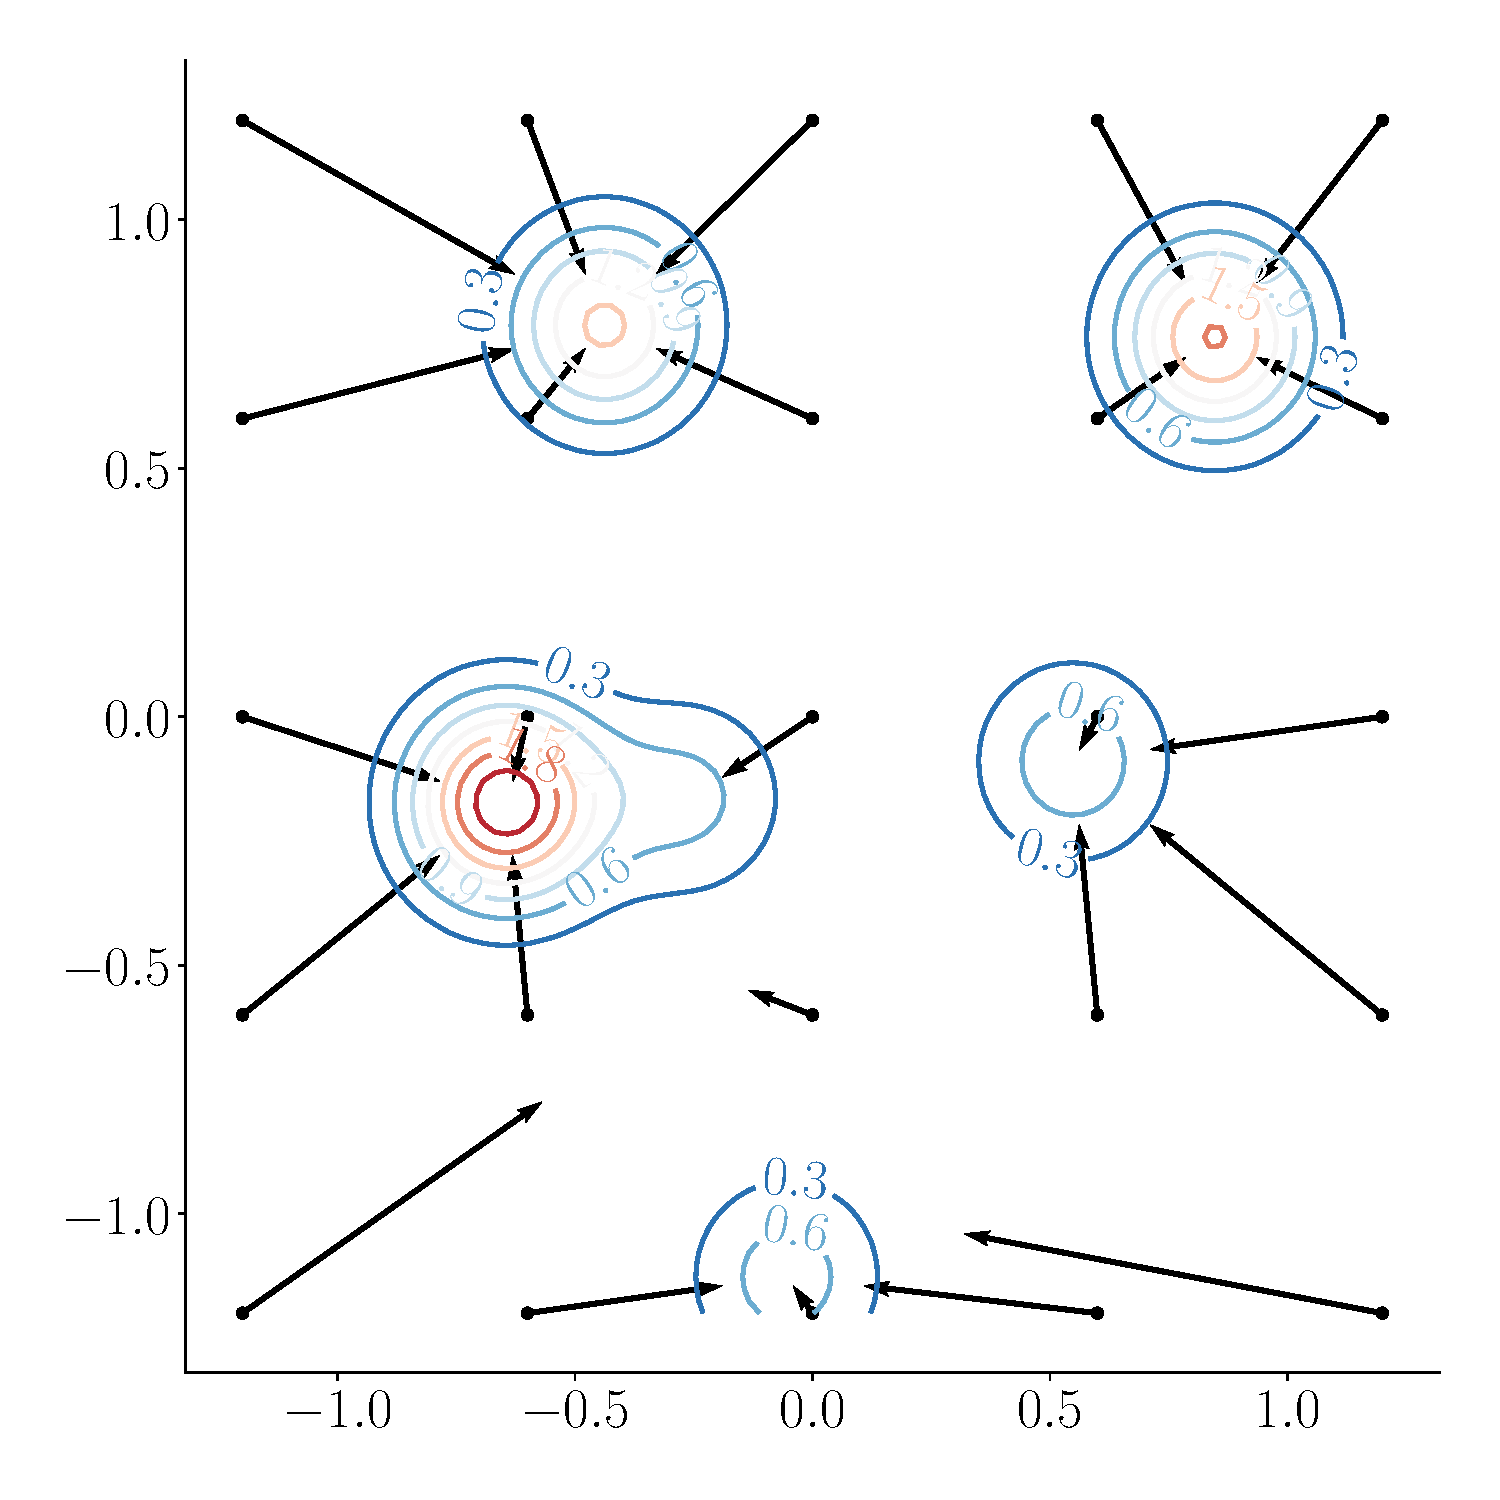
\includegraphics[width=.33\linewidth]{quiver/0.008}%
	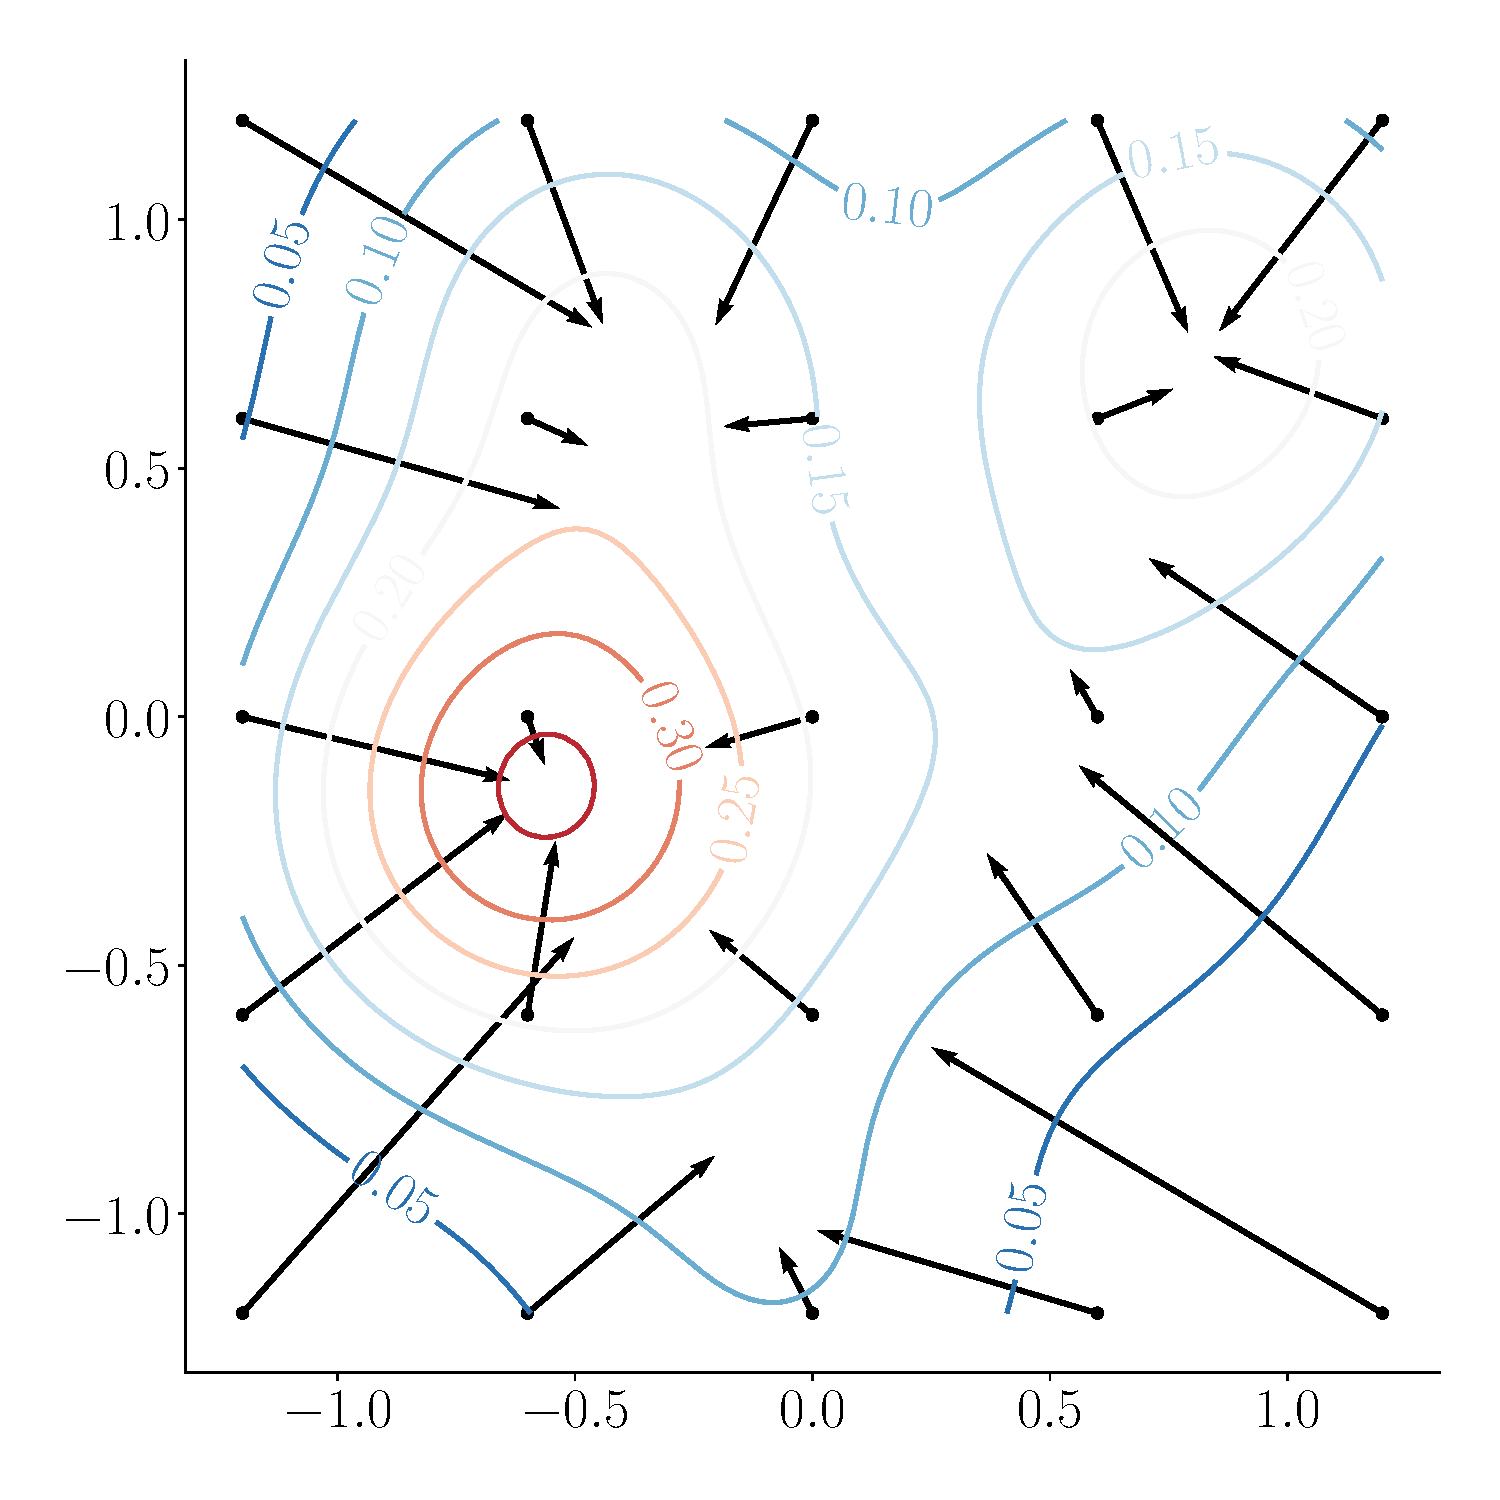
\includegraphics[width=.33\linewidth]{quiver/0.078}%
	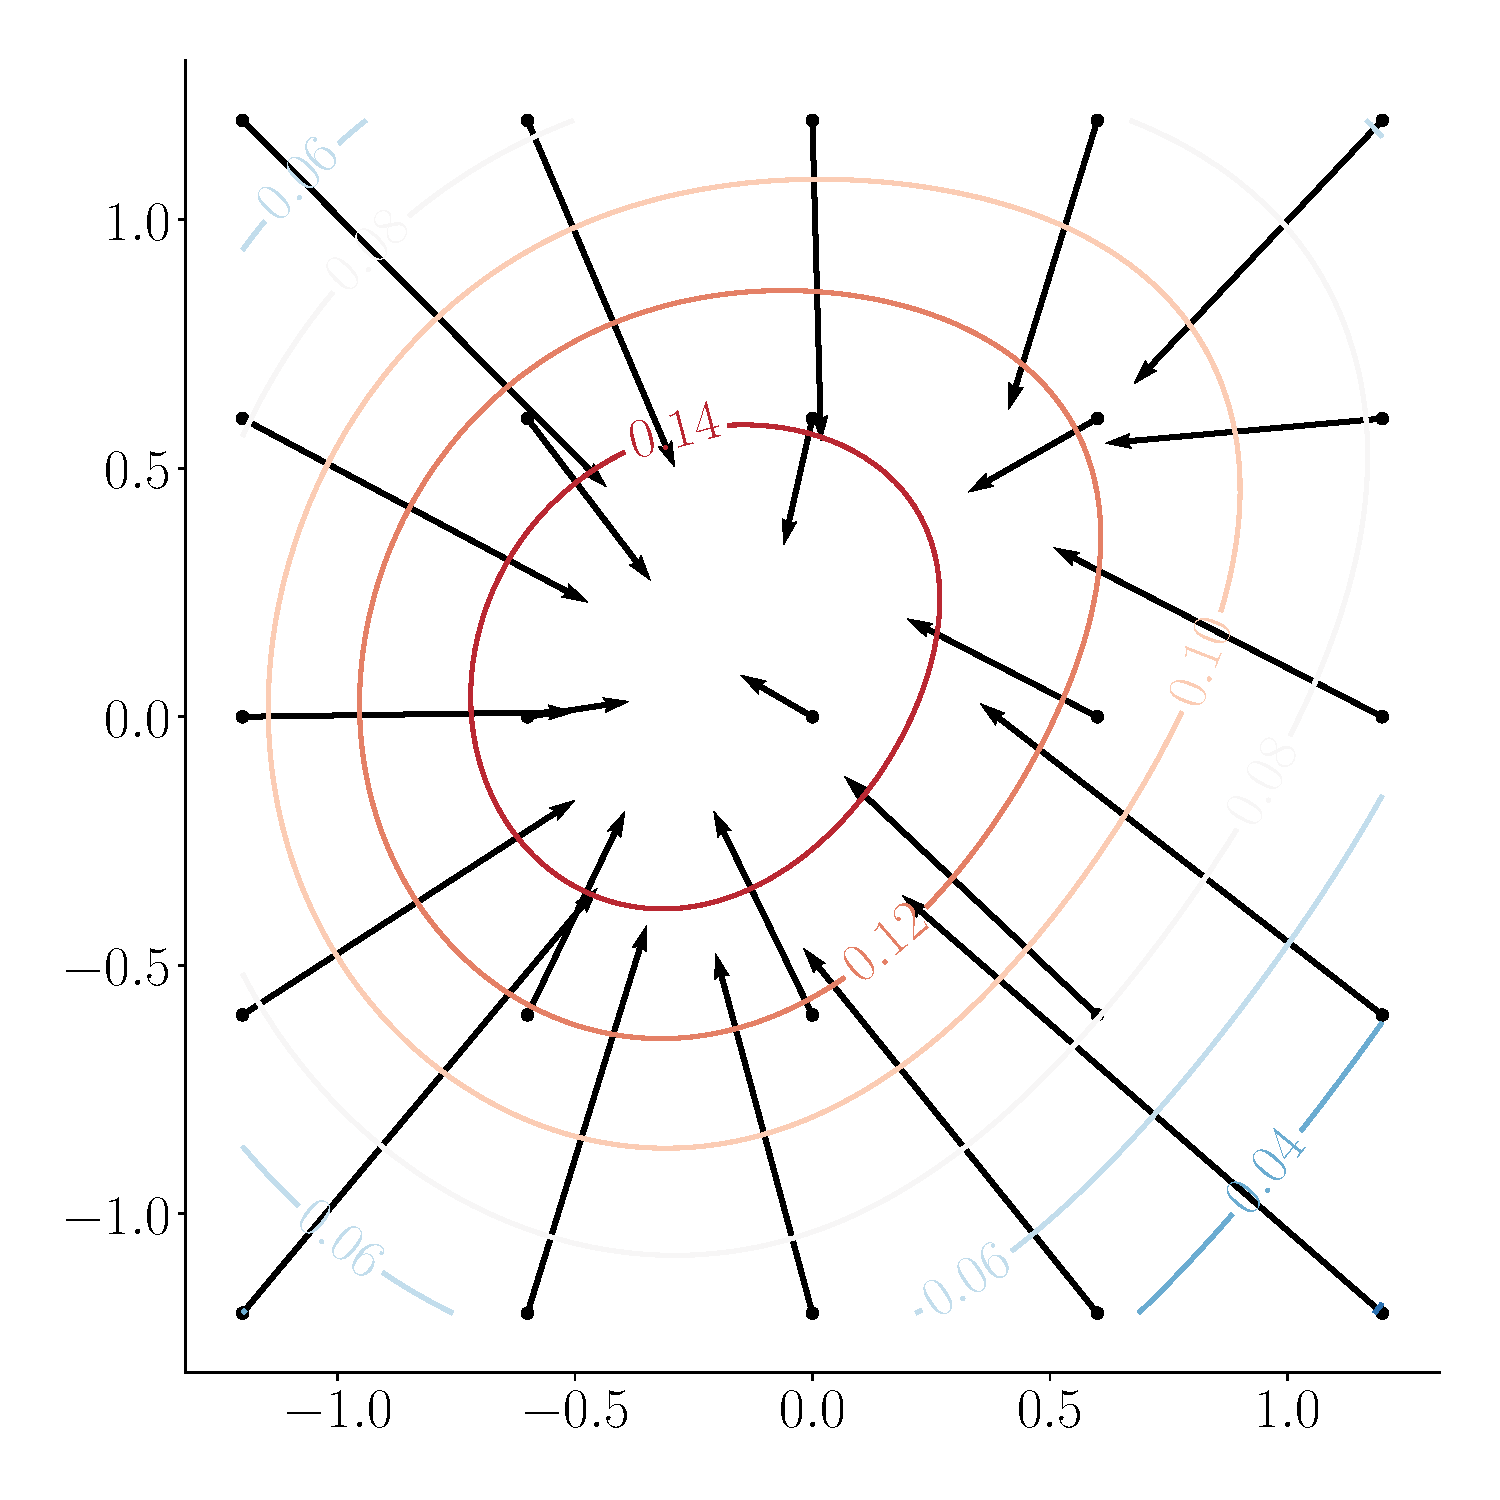
\includegraphics[width=.33\linewidth]{quiver/0.300}
	\caption[Example of the diffusion partial differential equation on an empirical density]{%
		 Diffusion of an empirical distribution consisting of weighted Dirac measures at diffusion times \( t = \num{0.008}, \num{0.078}, \num{0.3} \).
		 The arrows show the empirical Bayes estimate \( y \mapsto y + \num{2}t \nabla \log p_{Y_t}(y) \).
		As \( t \) approaches infinity, \( p_{Y_t} \) becomes log-concave and \( -\log p_{Y_t} \) approaches a quadratic function.
}%
	\label{fig:diffusion toy example}
\end{figure*}

Recently,~\eqref{eq:tweedie} has been used for parameter estimation~\cite{song_scorebased_2021,vincent_connection_2011}:
Let \( p_\theta : \mathcal{X} \times \rinterval{\num{0}}{\infty} \to \R_+ \) denote a parametrized model for which we wish that \( p_\theta(\argm, t) \approx p_{Y_t} \), for all \( t > \num{0} \).
Then, both the left- and right-hand side of~\eqref{eq:tweedie} are known in expectation, which leads to the loss function
\begin{equation}
\min_{\theta \in \Theta} \int_{\num{0}}^{\infty} \mathbb{E}_{(x, y_t) \sim p_{X, Y_t}} \bigl[ \norm{x - y_t - \sigma^{\num{2}}(t) \Grad_{1} \log p_\theta(y_t, t)}^{\num{2}} \bigr] \,\mathrm{d}t 
	\label{eq:score}
\end{equation}
for estimating \( \theta \) such that \( p_\theta(\argm, t) \approx p_{Y_t} \) for all \( t > \num{0} \).
Here, \( p_{X, Y_t} \) denotes the joint distribution of the clean and smoothed random variables.
Efficient sampling from this distribution is possible via ancestral sampling:
A pair \( (x, y_t) \sim p_{X, Y_t} \) can be constructed by sampling \( x \sim p_X \) and then computing \( y_t = x + \sqrt{\num{2}t}\eta \), where \( \eta \sim \NormalDistribution_{\num{0}, \Identity} \).
\( \Theta \) encodes constraints on the learnable parameters;
In our case, \( \Theta \) encodes constraints on the learnable parameters \( \theta \) that are required to be able to solve the diffusion \gls{pde}.

This learning problem is known as denoising score matching in the literature~\cite{song_scorebased_2021,vincent_connection_2011}.
It can be justified more formally as minimizing the Fisher divergence (\cref{def:fisher divergence}) of \( p_{Y_t} \) from \( p_\theta(\argm, t) \) for all \( t > \num{0} \):
\begin{equation}
	\begin{aligned}
		&\min_{\theta \in \Theta} \int_{\num{0}}^{\infty} \Fisher{p_{Y_t}}{p_\theta(\argm, t)}\,\mathrm{d}t = \\
		&\min_{\theta \in \Theta} \int_{\num{0}}^{\infty} \mathbb{E}_{y_t \sim p_{Y_t}} \bigl[ \norm{\Grad \log p_{Y_t}(y_t) - \Grad_{1} \log p_\theta(y_t, t)}^{\num{2}} \bigr] \,\mathrm{d}t
	\end{aligned}
	\label{eq:score fisher}
\end{equation}
where \( p_{Y_t} = G_{\num{0}, \num{2}t\Identity} * p_X \).
This is intractable as it is written since computing \( \nabla \log p_{Y_t} = \nabla \log (G_{\num{0},\num{2}t\Identity} * p_X) \) is complex.\footnote{%
	It has the infamous \enquote{log-integral-exp} structure.
	When \( p_X \) is an empirical distribution, this is the problem of computing the gradient of the kernel density estimate with a Gaussian kernel.
}
The key insight of the equivalence between the intractable formulation in~\cref{eq:score fisher} and the tractable \enquote{ancestral} formulation in~\cref{eq:score} is due to Vincent~\cite{vincent_connection_2011};
the proof is provided in their paper.
\section{Methods}%
\label{sec:methods pogmdm}
As mentioned in the introduction, we revisit the classical ridge-type structure of regularizers.
We endow them with a rigorous statistical interpretation and fit the potential functions by minimizing the Fisher divergence (\cref{def:fisher divergence}) from the reference density to the Gibbs density.
A suitable parametrization of the experts gives access to an \gls{mmse} optimal denoiser for Gaussian noise with arbitrary variance.
In the next section, we demonstrate our approach by learning a complete model on the space of image patches.
\subsection{A complete model on the space of image patches}%
\label{ssec:patch model}
We introduce the general concept of \glspl{pogmdm} through a complete model on the space of image patches.
We approximate the distribution of image patches of size~\( b\times b \) by a product of \( \NumExperts = b \times b \in \mathbb{N} \) one-dimensional experts.
In detail, the density on \( \R^{b\times b} \) is of the form
\begin{equation}
	\UndercompleteModel(x, t) = Z \bigl( \{ \Filter_k \}_{k=\num{1}}^\NumExperts, \sigma_{\num{0}}, t \bigr)^{-1}\prod_{k=\num{1}}^\NumExperts \Expert_k \bigl(\langle \Filter_k, x \rangle, w_j, t\bigr)
	\label{eq:gmdm patch}
\end{equation}
where~\( \Expert_{\num{1}}, \Expert_{\num{2}}, \dotsc, \Expert_\NumExperts \) are one-dimensional experts on the responses of linear filters \( \Filter_{\num{1}}, \Filter_{\num{2}}, \dotsc, \Filter_\NumExperts \in \R^{b \times b} \).
\( Z(\{ \Filter_k \}_{k=\num{1}}^\NumExperts,\sigma_{\num{0}}, t) \) the partition function ensuring that \( \UndercompleteModel \) is properly normalized.

The empirical Bayes construction discussed in~\cref{ssec:diffusion empirical bayes} requires finding \( \UndercompleteModel(\argm, t) =  G_{\num{0},\num{2}t\Identity} * \UndercompleteModel(\argm, \num{0}) \).
The closure properties of Gaussians under convolution motivates the choice of \emph{Gaussian mixture experts}.
In detail, the backbone of our models are one-dimensional Gaussian mixture experts~\( \map{\Expert_{\num{1}}, \Expert_{\num{2}}, \dotsc, \Expert_\NumExperts}{\R \times \Simplex^\NumComponents \times \rinterval{\num{0}}{\infty}}{\R_+} \) with \( \NumComponents \) components of the form
\begin{equation}
	\Expert_k(x, w_k, t) = \sum_{l=\num{1}}^{\NumComponents} w_{k,l} G_{\mu_l,\sigma_k^{\num{2}}(t)}(x).
	\label{eq:expert}
\end{equation}
For the experts to be normalized, the weights of each expert \( w_k = (w_{k,\num{1}}, w_{k, \num{2}}, \dotsc,\allowbreak w_{k, \NumComponents}) \) must be lie within the unit simplex \( \Simplex^\NumComponents \) (\cref{def:unit simplex}).
For simplicity, we assume that all experts have the same number of components and share the same means \( \mu_{\num{1}}, \mu_{\num{2}}, \dotsc, \mu_\NumComponents \in \R \), which are fixed a priori, see the details in~\cref{ssec:implementation details}.
In addition, within each expert, all components share the same variance.
This parametrization is versatile, as illustrated in \Cref{fig:parametrization examples}, and can  approximate classical sparsity-inducing potentials like the absolute, and value and the potentials of popular leptokurtic densities, such as the density of the Student-t distribution.
It also allows for multi-well potentials which are advantageous in Markov random field modeling~\cite{heess_learning_2009,zhu_minimax_1997} as discussed in the introduction.

\begin{figure}
	\begin{tikzpicture}
		\begin{groupplot}[
			group style={%
				group size=2 by 3,
				x descriptions at=edge bottom,
				y descriptions at=edge left,
				vertical sep=.2cm
			},
			ymin=-0.6,
			ymax=1.7,
			height=4cm,
			width=7cm,
		]
			\nextgroupplot
			\pgfplotsforeachungrouped \ccol in {1,3,...,125}
			{%
				\pgfmathparse{int(\ccol / 125 * 100)}
				\edef\tmp{%
					\noexpand\addplot [restrict y to domain=1e-3:inf, maincolor!\pgfmathresult!secondarycolor] table[col sep=comma, x index={0}, y index={\ccol}]{chapters/pogmdm/scripts/diffusion-illustration/abs.csv};%
				}\tmp%
			}%
			\addplot [black, thick] table[col sep=comma, x index={0}, y index={126}]{chapters/pogmdm/scripts/diffusion-illustration/abs.csv};%
			\nextgroupplot
			\addplot [black, thick] table[col sep=comma, x index={0}, y index={127}]{chapters/pogmdm/scripts/diffusion-illustration/abs.csv};%

			\nextgroupplot
			\pgfplotsforeachungrouped \ccol in {1,3,...,125}
			{%
				\pgfmathparse{int(\ccol / 125 * 100)}
				\edef\tmp{%
					\noexpand\addplot [restrict y to domain=1e-3:inf, maincolor!\pgfmathresult!secondarycolor] table[col sep=comma, x index={0}, y index={\ccol}]{chapters/pogmdm/scripts/diffusion-illustration/studentt.csv};%
				}\tmp%
			}%
			\addplot [black, thick] table[col sep=comma, x index={0}, y index={126}]{chapters/pogmdm/scripts/diffusion-illustration/studentt.csv};%
			\nextgroupplot
			\addplot [black, thick] table[col sep=comma, x index={0}, y index={127}]{chapters/pogmdm/scripts/diffusion-illustration/studentt.csv};%

			\nextgroupplot
			\pgfplotsforeachungrouped \ccol in {1,3,...,125}
			{%
				\pgfmathparse{int(\ccol / 125 * 100)}
				\edef\tmp{%
					\noexpand\addplot [restrict y to domain=1e-3:inf, maincolor!\pgfmathresult!secondarycolor] table[col sep=comma, x index={0}, y index={\ccol}]{chapters/pogmdm/scripts/diffusion-illustration/mhat.csv};%
				}\tmp%
			}%
			\addplot [black, thick] table[col sep=comma, x index={0}, y index={126}]{chapters/pogmdm/scripts/diffusion-illustration/mhat.csv};%
			\nextgroupplot
			\addplot [black, thick] table[col sep=comma, x index={0}, y index={127}]{chapters/pogmdm/scripts/diffusion-illustration/mhat.csv};%
		\end{groupplot}
	\end{tikzpicture}
	\caption[Examples of potentials represented by Gaussian mixture experts]{%
		The \gls{gmm} experts can model popular experts used in imaging:
		The Laplace expert (top), the Student-t expert (middle), and more general multimodal experts (bottom) are shown in the first column, and the corresponding absolute value potential (top), the leptokurtic Student-t potential (middle), and a Mexican-hat-like potential in the second column.
		Individual components of the \gls{gmm} are shown on the left, with the discretization as described in~\cref{ssec:implementation details} (\num{125} components, equidistant means over \( \interval{\num{-1}}{\num{1}} \), \( \sigma_{\num{0}}^{\num{2}} = \num{2}/(\num{125}-\num{1}) \)).
		To avoid clutter we only plot every second component.
	}%
	\label{fig:parametrization examples}
\end{figure}

Our main contribution is demonstrating that under certain assumptions, adapting the variances of the one-dimensional experts suffices to implement the convolution of \( \UndercompleteModel \) with a Gaussian.
Specifically, we show that the variance of the \( k \)-th expert, \( \sigma_k^{\num{2}} \), can be modeled as
\begin{equation}
	\sigma_k^{\num{2}}(t) = \sigma_{\num{0}}^{\num{2}} + c_k \num{2}t,
	\label{eq:variances}
\end{equation}
where \( \sigma_{\num{0}} > \num{0} \) is chosen a-priori to support the discretization of the means and \( c_k > \num{0} \) is derived from the filters \( \Filter_k \).

We leverage two well-known properties of Gaussians to determine how to adapt the variances of the one-dimensional experts with diffusion time \( t \).
First, the product of \glspl{gmm} is a \gls{gmm} up to normalization, see e.g.~\cite{1591840}, allowing us to work with expressive models that enable efficient \emph{evaluations} due to factorization.
Second, there exists an analytical solution to the diffusion \gls{pde} if \( p_X \) is a \gls{gmm}.
Green's function associated with the linear isotropic diffusion \gls{pde}~\eqref{eq:diff} is a Gaussian with isotropic covariance \( \num{2}t \Identity \).
Using previous notation, if \( X \) is a random variable with normal distribution \( \NormalDistribution_{\mu_X, \Sigma_X} \), then \( Y_t \) follows the distribution \( \NormalDistribution_{\mu_X, \Sigma_X + \num{2}t\Identity} \).\footnote{%
	Due to the linearity of the convolution, it suffices to consider a single Gaussian; the \gls{gmm} follows by a linear combination.
}
In particular, the mean remains unchanged and it suffices to adapt the covariance matrix with the diffusion time.

Due to closure properties of Gaussians under multiplication, \( \UndercompleteModel \) is a Gaussian mixture model on \( \R^{b\times b} \).
In order to find an expression for the variances of the one-dimensional Gaussian mixture experts under diffusion, we first establish the exact form of \( \UndercompleteModel(\argm, t) \) as a \gls{gmm} on \( \R^{b\times b} \).
We denote with \( \hat{l} : \{ 1, \dotsc, \NumExperts \} \to \{ 1, \dotsc, \NumComponents \}  \) a fixed but arbitrary selection from the index set \( \{ 1, \dotsc, \NumComponents \} \).
\begin{theorem}
	\( \UndercompleteModel(\argm, t) \) is a homoscedastic \gls{gmm} on \( \R^{b \times b} \) with precision
	\begin{equation}
		(\Sigma(t))^{-1} = \sum_{k=\num{1}}^\NumExperts \frac{1}{\sigma_k^{\num{2}}(t)} (\Filter_k \otimes \Filter_k).
		\label{eq:precision}
	\end{equation}
	It has \( \NumComponents^\NumExperts \) components whose means is identified by the choice of the index map \( \hat{l} \)
	\begin{equation}
		\mu_{\hat{l}} = \Sigma(t) \sum_{k=\num{1}}^\NumExperts \frac{1}{\sigma^{\num{2}}_k(t)}\Filter_k \mu_{\hat{l}(k)}.
	\end{equation}%
	\label{th:gmm}
\end{theorem}
\begin{proof}
	By inserting the definition of the one-dimensional \gls{gmm} experts,
	\begin{equation}
		\prod_{k=\num{1}}^\NumExperts \Expert_k \bigl( \langle \Filter_k, x \rangle, w_{j}, t \bigr) = \prod_{k=\num{1}}^\NumExperts \sum_{l=\num{1}}^{\NumComponents} \frac{w_{kl}}{\sqrt{\num{2}\pi\sigma_k^{\num{2}}(t)}} \exp\left(-\frac{1}{\num{2}\sigma_k^{\num{2}}(t)}{\bigl(\langle \Filter_k, x \rangle - \mu_l\bigr)}^{\num{2}} \right).
	\end{equation}
	We develop the product over the components and inspect a general term of the resulting sum, which corresponds to one component of the resulting \gls{gmm}.
	The general term of the resulting sum can be written as
	\begin{equation}
		\Biggl( \prod_{k=\num{1}}^\NumExperts \frac{w_{k\hat{l}(k)}}{\sqrt{\num{2}\pi\sigma_k^{\num{2}}(t)}} \Biggr) \exp\Biggl( -\sum_{k=\num{1}}^\NumExperts \frac{1}{\num{2}\sigma_k^{\num{2}}(t)} \bigl(\langle \Filter_k, x \rangle - \mu_{\hat{l}(k)}\bigr)^{\num{2}} \Biggr).
	\end{equation}
	To find the covariance, we match the gradient of the familiar quadratic form:
	\( \Grad_{x} \biggl(  \sum_{k=\num{1}}^\NumExperts \frac{1}{\num{2}\sigma_k^{\num{2}}(t)} \bigl(\langle \Filter_k, x \rangle - \mu_{\hat{l}(k)}\bigr)^{\num{2}} \biggr) = \sum_{k=\num{1}}^\NumExperts \frac{1}{\sigma_k^{\num{2}}(t)} \bigl( (\Filter_k \otimes \Filter_k) x - \Filter_k \mu_{\hat{l}(k)}\bigr) \).
	From the first term, we immediately identify \( (\Sigma(t))^{-1} = \sum_{k=\num{1}}^\NumExperts \frac{1}{\sigma_k^{\num{2}}(t)} (\Filter_k \otimes \Filter_k) \), and we find \( \mu_{\hat{l}} \) by left-multiplying \( (\Sigma(t)) \) onto \( \sum_{k=\num{1}}^\NumExperts \frac{1}{\sigma_k^{\num{2}}(t)} \Filter_k \mu_{\hat{l}(k)} \).
\end{proof}

As discussed in~\cref{ssec:diffusion empirical bayes}, the convolution of \( \UndercompleteModel \) with a Gaussian with covariance \( \num{2}t\Identity \) can be implemented by letting \( \Sigma(t) = \Sigma(\num{0}) + \num{2}t\Identity \).
Now, the challenge lies in finding a way to express this map by adapting the variances of the one-dimensional \gls{gmm} experts given the structure in~\cref{eq:gmdm patch}.
We show that this is not possible in the general case with an example on \( \R^{\num{2}} \):
Let \( \Filter_{\num{1}} = (\num{1}, \num{0}) \), \( \Filter_{\num{2}} = (\num{1}, \num{1}) / \sqrt{\num{2}} \), and \( \sigma_{\num{0}} = \num{1} \).\footnote{%
	For the sake of this example, the means are irrelevant.
}
Then, we have that
\begin{equation}
	\Filter_{\num{1}} \otimes \Filter_{\num{1}} = \begin{pmatrix}
		\num{1} & \num{0} \\
		\num{0} & \num{0}
		\end{pmatrix}\ \text{and}\ \Filter_{\num{2}} \otimes \Filter_{\num{2}} = \begin{pmatrix}
		\num{0.5} & \num{0.5} \\
		\num{0.5} & \num{0.5}
	\end{pmatrix},
\end{equation}
and at time \( t = \num{0} \),
\begin{equation}
	\Sigma^{-1} = \begin{pmatrix}
		\num{1.5} & \num{0.5} \\
		\num{0.5} & \num{0.5}
	\end{pmatrix}\ \text{and}\ \Sigma = \begin{pmatrix}
		\num{1} & \num{-1} \\
		\num{-1} & \num{3}
	\end{pmatrix}.
\end{equation}
At time \( t = \num{0.5} \),
\begin{equation}
	\Sigma + \Identity = \begin{pmatrix}
		\num{2} & \num{-1} \\
		\num{-1} & \num{4}
	\end{pmatrix}\ \text{and}\ (\Sigma + \Identity)^{\num{-1}} = \tfrac{1}{7} \begin{pmatrix}
		\num{4} & \num{1} \\
		\num{1} & \num{2}
	\end{pmatrix}.
\end{equation}
It is easy to see that \( (\Sigma + \Identity)^{-1} \) is not in the span of \( \Filter_{\num{1}} \otimes \Filter_{\num{1}} \) and \( \Filter_{\num{2}} \otimes \Filter_{\num{2}} \).
I.e., it can not be represented by \( \frac{1}{\sigma_{\num{1}}^{\num{2}}(t)} (\Filter_{\num{1}} \otimes \Filter_{\num{1}}) + \frac{1}{\sigma_{\num{2}}^{\num{2}}(t)} (\Filter_{\num{2}} \otimes \Filter_{\num{2}}) \), irrespective of the adaptation of the variances \( \sigma_{\num{1}}^{\num{2}} \) and \( \sigma_{\num{2}}^{\num{2}} \) of the one-dimensional \glspl{gmm}.

However, the next theorem establishes a tractable analytical expression for the diffusion process under the assumption of pair-wise orthogonal filters, i.e.\ that
\begin{equation}
	\langle \Filter_j, \Filter_i \rangle = \begin{cases}
		\num{0} & \text{if}\ i \neq j, \\
		\norm{\Filter_j}^{\num{2}} & \text{else},
	\end{cases}\ \text{for all}\ i, j \in \{ \num{1}, \dotsc, \NumExperts \}.
\label{eq:ortho}
\end{equation}
\begin{theorem}[Diffusion of a complete model]
	Under assumption~\eqref{eq:ortho}, \( \UndercompleteModel \) satisfies the diffusion \gls{pde} \( (\partial_t - \Delta_{\num{1}}) \UndercompleteModel(\argm, t) = \num{0} \) if the variances of the one-dimensional \gls{gmm} experts are adapted as \( \sigma_k^{\num{2}}(t) = \sigma_{\num{0}}^{\num{2}} + \norm{\Filter_k}^{\num{2}} \num{2}t \).
	\label{th:diff local}
\end{theorem}
\begin{proof}
	We exploit that the orthogonality assumption on the filters,~\eqref{eq:ortho}, immediately gives the Eigendecomposition of the precision:
	At \( t = \num{0} \), the Eigendecomposition of the precision is
	\begin{equation}
		(\Sigma(\num{0}))^{-1} = \sum_{k=\num{1}}^\NumExperts \frac{\norm{\Filter_k}^{2}}{\sigma_{\num{0}}^{\num{2}}} \biggl(\frac{\Filter_k}{\norm{\Filter_k}} \otimes \frac{\Filter_k}{\norm{\Filter_k}} \biggr).
	\end{equation}
	The covariance can be computed by taking the reciprocal of the Eigenvalues:
	\begin{equation}
		\Sigma(\num{0}) = \sum_{k=\num{1}}^\NumExperts \frac{\sigma_{\num{0}}^{\num{2}}}{\norm{\Filter_k}^{2}} \biggl(\frac{\Filter_k}{\norm{\Filter_k}} \otimes \frac{\Filter_k}{\norm{\Filter_k}}\biggr).
	\end{equation}
	Adding a multiple of the identity to the covariance can be expressed on the level of Eigenvalues as
	\begin{equation}
		\Sigma(\num{0}) + \num{2}t\Identity = \sum_{k=\num{1}}^\NumExperts \frac{\sigma_{\num{0}}^{\num{2}} + \num{2}t\norm{\Filter_k}^{2}}{\norm{\Filter_k}^{2}} \biggl(\frac{\Filter_k}{\norm{\Filter_k}} \otimes \frac{\Filter_k}{\norm{\Filter_k}}\biggr),
	\end{equation}
	and inverting is again just taking the reciprocal of the Eigenvalues:
	\begin{equation}
		\begin{aligned}
			(\Sigma(\num{0}) + \num{2}t\Identity)^{-1} &= \sum_{k=\num{1}}^\NumExperts \frac{\norm{\Filter_k}^{2}}{\sigma_{\num{0}}^{\num{2}} + \num{2}t\norm{\Filter_k}^{2}} \biggl(\frac{\Filter_k}{\norm{\Filter_k}} \otimes \frac{\Filter_k}{\norm{\Filter_k}}\biggr) \\
												 &= \sum_{k=\num{1}}^\NumExperts \frac{1}{\sigma_{\num{0}}^{\num{2}} + \num{2}t\norm{\Filter_k}^{{\num{2}}}} (\Filter_k \otimes \Filter_k).
		\end{aligned}
		\label{eq:prec diff undercomplete}
	\end{equation}
	This is exactly of the form of~\cref{eq:precision}, with \( \sigma_k^{\num{2}}(t) = \sigma_{\num{0}}^{\num{2}} + \norm{\Filter_k}^{\num{2}} \num{2}t \).
	Thus, \( \UndercompleteModel \) satisfies the diffusion \gls{pde} if \( \sigma_k^{\num{2}}(t) = \sigma_{\num{0}}^{\num{2}} + \norm{\Filter_k}^{\num{2}} \num{2}t \).
\end{proof}

Denoting with \( X \) the random variable whose density we aim to model at time \num{0}, we argued in~\cref{ssec:correct way to think about marginals} that in general, the one-dimensional expert acting on \( \inprod{\Filter_k}{\argm} \) does not model the distribution of the random variable \( \inprod{\Filter_k}{X} \).
However, in the undercomplete case with orthogonal filters, this is the case:
\begin{corollary}%
	\label{cor:marginal}
	Let \( X \) be the random variable whose density we model with~\cref{eq:gmdm patch}, and let \( Y_t \) be the random variable given by~\cref{eq:pogmdm diffusion}.
	Then, with assumption~\eqref{eq:ortho} the experts \( \Expert_k(\argm, w_k, t) \) in~\eqref{eq:gmdm patch} model the marginal distribution of the random variable \( U_{k, t} = \langle \Filter_k, Y_t \rangle \) for any \( t \geq \num{0} \).
\end{corollary}
\begin{proof}
	Consider the component of the resulting homoscedastic \gls{gmm} identified by the choice of the index map \( \hat{l} \): \( Y_{\hat{l}, t} \sim \NormalDistribution_{\mu_{\hat{l}}, \Sigma + \num{2}t\Identity} \).
	The distribution of \( \hat{U}_{k, t} = \langle \Filter_k, Y_{\hat{l}, t} \rangle \) is \( \hat{U}_{k, t} \sim \NormalDistribution_{\inprod{\Filter_k}{\mu_{\hat{l}}}, \inprod{\Filter_k}{(\Sigma + \num{2}t\Identity) \Filter_k}} \) (see e.g.\ \cite[theorem 3.1]{Gut2009}).
	Under our orthogonality assumptions, this simplifies to \( \NormalDistribution_{\mu_{\hat{l}(k)}, \sigma_{\num{0}}^{\num{2}}  + \num{2}t\norm{\Filter_k}^{\num{2}}} \).
	The claim follows from the linear combination of the different components.
\end{proof}
In addition, we can compute the normalization constant of \( \UndercompleteModel(\argm, t) \) for any \( t \geq \num{0} \) as
\begin{equation}
	Z\bigl(\{ \Filter_k \}_{k=\num{1}}^\NumExperts, \sigma_{\num{0}}, t\bigr) = \sqrt{\prod_{k=\num{1}}^\NumExperts \num{2} \pi \frac{\sigma_{\num{0}}^{\num{2}} + \num{2}t\norm{\Filter_k}^{\num{2}}}{\norm{\Filter_k}^{\num{2}}}},
\end{equation}
which is just the square root of the product of the eigenvalues in~\cref{eq:prec diff undercomplete} multiplied by \( \num{2}\pi \).

We presented the analysis above assuming that the number of one-dimensional experts is exactly equal to the dimensionality of the space; a complete model.
Coupled with the orthogonality constraint, this effectively ensures that the distribution is \emph{proper}.
However, in practice fewer experts can be utilized, for instance to enforce invariance with respect to radiometric shifts.\footnote{%
	In this case, there are \( b^{\num{2}} - \num{1} \) experts acting on the responses of zero-mean filters;
	we do this in~\cref{sssec:orthogonal filters}.
}
In this case, \( \UndercompleteModel(\argm, t) \) does not admit a density with respect to the Lebesgue measure for any \( t \geq \num{0} \).
Nevertheless, the theoretical analysis can be carried out by restricting the Lebesgue measure to the span of the filters (invoking the disintegration theorem) and replacing inverses by pseudo-inverses and determinants by pseudo-determinants~\cite{Rao1973}.
\subsection{Wavelet model}%
\label{ssec:wavelet model}
The key ingredient in the previous section was the orthogonality of the filters.
In other words, the filters \( \Filter_{\num{1}}, \Filter_{\num{2}}, \dotsc, \Filter_\NumExperts \) form an orthogonal (not necessarily orthonormal) basis for (possibly a subspace of) \( \R^{b\times b} \).
In this section, we discuss the application of explicit diffusion models in another well-known orthogonal basis:
Wavelets.

A brief discussion about the wavelet transform can be found in ~\cref{ssec:wavelet transform};
for the purposes of this section it suffices to note that any image \( x \in \R^{\Height \times \Width} \) can be decomposed as
\begin{equation}
	x = \proj_{V_m} x + \sum_{j\leq m}\proj_{W_j} x
	\label{eq:wavelet decomposition}
\end{equation}
where \( \map{\proj_{W_{\num{1}}}, \proj_{W_{\num{2}}},\dotsc, \proj_{W_m}}{\R^{\Height \times \Width}}{\R^{\Height \times \Width}} \) are the projections onto the \emph{orthogonal detail spaces} \( W_{\num{1}}, W_{\num{2}}, \dotsc, W_m \) .
We utilize the shorthand notation
\begin{equation}
	\mathcal{W}_j = \proj_{W_j},
\end{equation}
and recall the properties of an orthogonal projection,
\begin{alignat}{3}
	&\text{(self-adjoint)} &&(\mathcal{W}_j)^\ast &&= \mathcal{W}_j, \nonumber \\
	&\text{(idempotency)} &&\mathcal{W}_j \circ \mathcal{W}_j &&= \mathcal{W}_j,\ \text{and} \label{eq:projection}\\
	&\text{(identity on subspace)}\ \ \ &&\mathcal{W}_j|_{W_j} &&= \Identity_{W_j}\nonumber 
\end{alignat}
where \( \mathcal{W}_j|_{W_j} \) denotes the restriction of \( \mathcal{W}_j \) to \( W_j \).

As in the previous section, we model the wavelet-responses with Gaussian mixture experts.
For simplicity, we discard the partition function and build an undercomplete model on \( \oplus_{j=\num{1}}^\NumExperts W_j \):\footnote{%
	Again, this could be more formally dealt with via the disintegration theorem.
}
\begin{equation}
	\WaveletModel(x, t) \propto \prod_{i,j=\num{1}}^{\Height, \Width} \prod_{k=\num{1}}^{\NumExperts} \Expert_k \bigl((\mathcal{W}_k x)_{i, j}, w_k, t\bigr).
	\label{eq:wavelet gmm}
\end{equation}

Following the approach utilized in~\cref{th:diff local}, we first describe the exact form of~\eqref{eq:wavelet gmm} as a \gls{gmm} on \( \R^n \).
\begin{theorem}
	\( \WaveletModel(\argm, t) \) is a homoscedastic \gls{gmm} on \( \ImgDim \) with precision
	\begin{equation}
		(\Sigma(t))^{-1} =  \sum_{k=\num{1}}^\NumExperts \frac{1}{\sigma_k^{\num{2}}(t)} \mathcal{W}_k.
	\end{equation}
	\label{prf:wavelet gmm}
\end{theorem}
\begin{proof}
	As in ~\cref{th:diff local}, this follows immediately from the expansion of~\cref{eq:wavelet gmm}:
	\begin{equation}
		\WaveletModel(x, t) \propto \prod_{i,j=\num{1}}^{\Height,\Width} \prod_{k=\num{1}}^\NumExperts \sum_{l=\num{1}}^{\NumComponents} \frac{w_{kl}}{\sqrt{\num{2}\pi\sigma_k^{\num{2}}(t)}} \exp\left(-\frac{((\mathcal{W}_k x)_{i, j} - \mu_l)^{\num{2}}}{\num{2}\sigma_k^{\num{2}}(t)}\right).
		\label{eq:conv gmm}
	\end{equation}
	By expanding the product over the features as well as the experts we find that the general component has the form\footnote{%
		Expressions for the weight and the mean \( \mu_{\hat{l}(i, j, k)} \in \ImgDim \) of this component can be derived easily but are omitted for simplicity.
	}
	\begin{equation}
		\exp\left(-\sum_{k=\num{1}}^\NumExperts \frac{\num{1}}{\num{2}\sigma_k^{\num{2}}(t)}\norm{\mathcal{W}_k x - \mu_{\hat{l}(i, j, k)}}^{\num{2}}\right).
		\label{eq:expanded}
	\end{equation}
	The precision of this component is
	\begin{equation}
		(\Sigma(t))^{-1} = \sum_{k=\num{1}}^\NumExperts \frac{\num{1}}{\sigma_k^{\num{2}}(t)} \bigl(\mathcal{W}_k \bigr)^\ast \mathcal{W}_k,
		\label{eq:prec rn}
	\end{equation}
	which simplifies to
	\begin{equation}
		(\Sigma(t))^{-1} = \sum_{k=\num{1}}^\NumExperts \frac{\num{1}}{\sigma_k^{\num{2}}(t)} \mathcal{W}_k
		\label{eq:wavelet prec}
	\end{equation}
	since projections are self-adjoint and idempotent, see~\eqref{eq:projection}.
\end{proof}
It remains to show how the \( \Sigma(t) = \Sigma(\num{0}) + \num{2}t\Identity \) can be implemented by adapting the variances of the one-dimensional Gaussian mixture experts.
However, this becomes trivial due to the orthogonality of the detail spaces.
\begin{theorem}[Wavelet diffusion]%
	\label{th:wavelet diff}
	\( \WaveletModel(\argm, t) \) satisfies the diffusion \gls{pde} \( (\partial_t - \Delta_{\num{1}}) \WaveletModel(\argm, t) = \num{0} \) if the variances of the one-dimensional Gaussian mixture experts are adapted as \( \sigma_k^{\num{2}}(t) = \sigma_{\num{0}}^{\num{2}} + \num{2}t \).
\end{theorem}
\begin{proof}
	Due to the orthogonality of the detail spaces, the precision in~\cref{eq:wavelet prec} on \( \oplus_{k=\num{1}}^\NumExperts W_k \) is the identity (see also the decomposition~\cref{eq:wavelet decomposition}).
	Thus, it suffices to adapt the variance of the one-dimensional \glspl{gmm} \( \Expert_k \) with \( \sigma_k^{\num{2}}(t) = \sigma_{\num{0}}^{\num{2}} + \num{2}t \).
\end{proof}
We can endow the different sub-bands of the wavelet transformation with scalars to weight their influence as follows:
Replacing \( \mathcal{W}_k \) with \( \lambda_k \mathcal{W}_k \) in~\eqref{eq:prec rn} (the derivation does not change up to this point), we find that the diffusion \gls{pde} is satisfied when \( \sigma_k^{\num{2}}(t) = \sigma_{\num{0}}^{\num{2}} + \num{2}t \lambda_k^{\num{2}} \).
Thus, the scaling parameters \( \lambda_{k} \) are analogous to the filter-norms in~\cref{th:diff local}.

In the above, we played a slight of hand by using the one-dimensional theory from the preliminaries in a two-dimensional context.
However, the derivation is essentially the same for the two-dimensional wavelet transform by replacing the detail index (\( k \) in the above) with a two-index to account for the direction (vertical, horizontal, diagonal).
The details are discussed in slightly more detail in the original publication~\cite{zach_pogmdm_2024} and rigorously in~\cite[chapter 4.4]{bredies_mathematical_2018}.
\subsection{Overcomplete model}%
\label{ssec:conv model}
The undercomplete model on filter-responses discussed in~\cref{ssec:patch model} can not account for the correlation of overlapping patches when used for whole image restoration~\cite{RoBl09,zoran_learning_2011}.
Similarly, the model based on wavelet-responses is limited in expressiveness since it only models the distribution of a scalar random variable per sub-band.
In what follows, we describe a convolutional \gls{pogmdm} that avoids the extraction and combination of patches in patch-based image priors and can account for the local nature of low-level image features.

In analogy to the product-of-experts-type model acting on filter-responses, here we extend the \gls{foe} model~\cite{RoBl09} to our considered diffusion setting by accounting for the diffusion time~\( t \) and obtain
\begin{equation}
	\OvercompleteModel(x, t) \propto \prod_{i,j=\num{1}}^{\Height,\Width} \prod_{k=\num{1}}^\NumExperts \Expert_k \bigl((K_k x)_{i, j}, w_{k}, t\bigr).
	\label{eq:gmdm}
\end{equation}
Here, the experts~\( \Expert_{\num{1}}, \Expert_{\num{2}}, \dotsc, \Expert_\NumExperts \) act the responses to convolution operators \( \map{K_{\num{1}}, K_{\num{2}}, \dotsc,\allowbreak K_\NumExperts}{\R^{\Height\times\Width}}{\R^{\Height\times\Width}} \).
In detail, the convolution operators implement circular boundary conditions and hence are circulant Toeplitz operators (see~\cite[section 5.5.2]{Nikolski2020-dx}) described by
\begin{equation}
	(K_k x)_{i, j} = \sum_{p, q=\num{1}}^{b, b} (\Filter_k)_{p, q} \cdot x_{\imath(p), \jmath(q)},
\end{equation}
where\footnote{%
	Here, \( \mod \) is understood as the least positive residue, e.g. \( \num{-1} \mod \num{5} = \num{4} \).
}
\begin{equation}
	 \imath(p) = \num{1} + (i - p + \lfloor b / \num{2} \rfloor) \mod \Height 
\end{equation}
and
\begin{equation}
	\jmath(q) = \num{1} + (j - q + \lfloor b / \num{2} \rfloor) \mod \Width.
\end{equation}
Further, \( w_k \in \Simplex^\NumComponents \) are the weights of the components of the \( k \)-th expert \( \Expert_k \) (see~\eqref{eq:expert}).
In the above, \( \Filter_{\num{1}}, \Filter_{\num{2}}, \dotsc, \Filter_\NumExperts \in \R^{b \times b} \) are the \( b \times b \) filters of the respective convolution operators.
As with the models based on filter- and wavelet-responses, under some assumptions on the convolution operators it suffices to adapt the variances \( \sigma_k^{\num{2}} \) by the diffusion time, which we show by the following analysis.

We start by outlining the structure of \eqref{eq:gmdm} as a \gls{gmm} on \( \R^{\Height \times \Width} \).
\begin{theorem}
	\( \OvercompleteModel(\argm, t) \) is a homoscedastic \gls{gmm} on \( \R^{\Height \times \Width} \) with precision
	\begin{equation}
		(\Sigma(t))^{-1} = \sum_{k=\num{1}}^\NumExperts \frac{1}{\sigma_k^{\num{2}}(t)} \Adjoint{K_k}K_k.
		\label{eq:prec overcomplete}
	\end{equation}%
	\label{th:overcomplete gmm}
\end{theorem}
\begin{proof}
	The proof is essentially given in the proof of~\cref{prf:wavelet gmm}:
	The form of the covariance matrix above is~\cref{eq:prec rn}, which holds for general linear operators.
\end{proof}

As previously, the challenge now lies in finding a way to express the map \( \Sigma(t) = \Sigma(\num{0}) + \num{2}t\Identity \) by adapting the variances of the one-dimensional Gaussian mixture experts.
The next theorem establishes an analytic expression for the diffusion process under the following assumption:
The frequency spectra of the filters \( \Filter_{\num{1}}, \Filter_{\num{2}}, \dotsc, \Filter_\NumExperts \) are non-overlapping and constant on the support.
More formally, let the size of the filters be \( b \times b \) and let the image size be \( \Height \times \Width \).
Let \( \map{P}{\R^{b\times b}}{\R^{\Height \times \Width}} \) be a padding and shifting operator\footnote{%
	This padding operator is formally needed for the convolution theorem to hold in the next theorem.
	In practice, we will use filters that are directly defined in the frequency domain, see~\cref{ssec:learning shearlets}.
}
\( P = \tilde{P} S \) where \( \map{\tilde{P}}{\R^{b\times b}}{\R^{m\times n}} \) is zero padding (putting the filter in the upper left hand corner) and \( (Sx)_{i, j} = x_{\imath(\lfloor b /\num{2}\rfloor), \jmath(\lfloor b/\num{2} \rfloor)} \).
Then, denoting by \( \Gamma_k \) the support of \( \Fourier P \Filter_k \), that is \( \Gamma_k = \Set{(i, j) \given (\Fourier P \Filter_k)_{i, j} \neq \num{0}} \), we require that
\begin{equation}
	\Gamma_k \cap \Gamma_l = \emptyset\ \text{for all}\ k,l=\num{1},\num{2},\dotsc,\NumExperts\ \text{where}\ k \neq l.
	\label{eq:disjoint}
\end{equation}
In addition, let
\begin{equation}
	\bigl(|\Fourier P \Filter_k|\bigr)_{i, j} = \xi_k \chi_{\Gamma_k}\bigl((i, j)\bigr),
	\label{eq:constant}
\end{equation}
where \( \xi_k > \num{0} \) is the magnitude and \( \chi_{\Gamma_k} \) is the characteristic function (\cref{def:characteristic function}) of \( \Gamma_k \).
In the language of classical signal processing, the filters \( k_{\num{1}}, k_{\num{2}}, \dotsc, k_\NumExperts \) should be \emph{ideal}\footnote{up to scaling; typically ideal filters have no gain in their passband}, see~\cite[fig. 2.17, fig. 2.18]{oppenheim2009discrete};
we discuss the implications of this in after the theorem.
\begin{theorem}[Diffusion of an overcomplete model]
	Under assumptions~\eqref{eq:disjoint} and~\eqref{eq:constant}, \( \OvercompleteModel \) satisfies the diffusion \gls{pde} \( (\partial_t - \Delta_{\num{1}}) \OvercompleteModel(\argm, t) = \num{0} \) if the variances of the one-dimensional Gaussian mixture experts are adapted as \( \sigma_k^{\num{2}}(t) = \sigma_{\num{0}}^{\num{2}} + \xi_k^{\num{2}} \num{2}t \).
	\label{th:overcomplete diffusion}
\end{theorem}
\begin{proof}
	To efficiently invert the precision, we exploit a diagonalization of the circulant Toeplitz convolution operators \( K_{\num{1}}, K_{\num{2}}, \dotsc, K_{\NumExperts} \) via the discrete Fourier transform.
	The convolution operators are diagonalized as (see~\cite[section 5.5.4]{Nikolski2020-dx})
	\begin{equation}
		K_k = \Adjoint{\Fourier} \diag(\Fourier P \Filter_k) \Fourier.
	\end{equation}
	Thus, the precision in~\cref{eq:prec overcomplete} can be expressed as
	\begin{equation}
		\begin{aligned}
			(\Sigma(t))^{-1} &= \sum_{k=\num{1}}^{\NumExperts} \frac{1}{\sigma_k^{\num{2}}(t)} \Adjoint{(\Adjoint{\Fourier} \diag(\Fourier P \Filter_k) \Fourier)}\Adjoint{\Fourier} \diag(\Fourier P \Filter_k) \Fourier \\
							 &= \sum_{k=\num{1}}^{\NumExperts} \frac{1}{\sigma_k^{\num{2}}(t)} \Adjoint{\Fourier} \diag(\conj{\Fourier P \Filter_k}) \diag(\Fourier P \Filter_k) \Fourier \\
							 &= \Adjoint{\Fourier}\diag\biggl(\sum_{k=\num{1}}^\NumExperts \frac{|\Fourier P \Filter_k|^{\num{2}}}{\sigma^{\num{2}}_k(t)}\biggr) \Fourier,
		\end{aligned}
		\label{eq:fourier diagonalization}
	\end{equation}
	where we used that \( \Fourier \Adjoint{\Fourier} = \Identity \) and \( \conj{z}z = |z|^{\num{2}} \).
	To compute the covariance at time zero, it suffices to invert the diagonal operator:
	\begin{equation}
		\Sigma(\num{0}) = \Adjoint{\Fourier}\diag\biggl(\sum_{k=\num{1}}^\NumExperts \frac{|\Fourier P \Filter_k|^{\num{2}}}{\sigma^{\num{2}}_{\num{0}}}\biggr)^{-1} \Fourier.
	\end{equation}
	Critically, at each entry of the diagonal operator only one filter is active:
	\begin{equation}
		\biggl( \sum_{k=\num{1}}^\NumExperts \frac{|\Fourier P \Filter_k|^{\num{2}}}{\sigma^{\num{2}}_{\num{0}}} \biggr)_{i, j} = \frac{|\Fourier P \Filter_{a}|^{\num{2}}}{\sigma^{\num{2}}_{\num{0}}}\ \text{where \( a \) is such that}\ (i, j) \in \Gamma_a.
	\end{equation}
	Thus, the covariance is
	\begin{equation}
		\Sigma(\num{0}) = \Adjoint{\Fourier}\diag\biggl(\sum_{k=\num{1}}^\NumExperts \frac{\sigma^{\num{2}}_{\num{0}}}{|\Fourier P \Filter_k|^{\num{2}}}\biggr) \Fourier
	\end{equation}
	and adding a multiple of the identity amounts to
	\begin{equation}
		\Sigma(\num{0}) + \num{2}t\Identity = \Adjoint{\Fourier}\diag\biggl(\sum_{k=\num{1}}^\NumExperts \frac{\sigma^{\num{2}}_{\num{0}} + \num{2}t|\Fourier P \Filter_k|^{\num{2}}}{|\Fourier P \Filter_k|^{\num{2}}}\biggr) \Fourier.
	\end{equation}
	Finally, for the same reason as previously this can be inverted as
	\begin{equation}
		(\Sigma(\num{0}) + \num{2}t\Identity)^{-1} = \Adjoint{\Fourier}\diag\biggl(\sum_{k=\num{1}}^\NumExperts \frac{|\Fourier P \Filter_k|^{\num{2}}}{\sigma^{\num{2}}_{\num{0}} + \num{2}t|\Fourier P \Filter_k|^{\num{2}}}\biggr) \Fourier.
	\end{equation}
	This is exactly of the form~\cref{eq:fourier diagonalization} with \( \sigma_k(t) = \sigma_{\num{0}}^{\num{2}} + \num{2}t\xi_k^{\num{2}} \).
\end{proof}

The overcomplete model~\eqref{eq:gmdm} is fundamentally different from the model based on filter-responses discussed in~\cref{ssec:patch model}.
Specifically, the one-dimensional \gls{gmm} experts \( \Expert_k(\argm, w_k, t) \) do \emph{not} model the distribution of the filter-responses of their corresponding filter kernels \( \Filter_k \).
Instead, the \enquote{overcompleteness through convolution} allows the model to capture the non-trivial correlation of overlapping patches.

The next step is to select filters \( k_{\num{1}}, k_{\num{2}}, \dotsc, k_\NumExperts \) that meet our assumptions.
One approach might be to construct ideal filters by partitioning the Fourier spectrum, aligning with our assumption.
However, this does leads to filters with infinite spatial support, making the construction impractical:
The \gls{mrf}-type models~\eqref{eq:gmdm} aim to share potential for responses extracted at different locations, requiring filters much smaller than the image.
Conversely, any finite-length filter's spectrum has infinite support and special care is needed to ensure spectra of different filters do not overlap.
This issue is related to the classical windowing problem, see~\cite[section 7.5]{oppenheim2009discrete} and~\cref{fig:windowing}.
\begin{figure*}
	\centering
	\begin{tikzpicture}
		\begin{scope}[xshift=-4cm]
			\node at (0, 0) {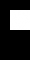
\includegraphics[height=3cm]{../scripts/convolutions/prescribed-spectrum/spectrum_magnitude}};
			\node at (0, -1.8) {Magnitude};
			\node at (2, 0) {
\includegraphics[height=3cm]{../scripts/convolutions/prescribed-spectrum/spectrum_phase}};
			\node at (2, -1.8) {Phase};
			\node at (4.75, 0) {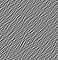
\includegraphics[height=3cm]{../scripts/convolutions/prescribed-spectrum/time}};
			\node at (4.75, -1.8) {Filter};
		\end{scope}
		\draw [ultra thick, gray] (2.75, 1.75) -- (2.75, -2);
		\begin{scope}[xshift=4cm]
			\node at (0, 0) {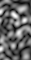
\includegraphics[height=3cm]{../scripts/convolutions/prescribed-filter/spectrum_magnitude}};
			\node at (0, -1.8) {Magnitude};
			\node at (2, 0) {
\includegraphics[height=3cm]{../scripts/convolutions/prescribed-filter/spectrum_phase}};
			\node at (2, -1.8) {Phase};
			\node at (4.75, 0) {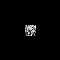
\includegraphics[height=3cm]{../scripts/convolutions/prescribed-filter/time}};
			\node at (4.75, -1.8) {Filter};
		\end{scope}
	\end{tikzpicture}
	\caption[Windowing in time- and frequency domain]{%
		Windowing leads to infinite support in the transformed domain:
		On the left, a partitioning of the spectrum is prescribed, which leads to a filter with image-sized support.
		On the right, the finite-support filter is prescribed, which leads to a spectrum with image-sized support.
		Since we assume real filters, we only show half of the spectrum as it enjoys conjugate symmetry.
	}%
	\label{fig:windowing}
\end{figure*}

We balance the trade-off between satisfying theoretical assumptions on the spectra and having compactly supported time-domain filters, by using compactly supported shearlets~\cite{kutyniok_shearlets_2012,lim_discrete_2010}, specifically the non-separable version from~\cite{lim_nonseparable_2013}.
As an extension to the wavelet transform, the shearlet transform represents directional information in multidimensional signals via shearing and provides an optimally sparse representation of signals within a certain smoothness class~\cite{Guo2007,KUTYNIOK20111564}.
We use the non-separable digital shearlet transform~\cite{lim_nonseparable_2013}, an improved discretization of the compactly supported shearlets introduced by Lim in~\cite{lim_discrete_2010}.
The induced frequency tiling is schematically shown in~\cref{fig:shearlet partitioning}, where the frequency plane is partitioned into non-overlapping cones indexed by the scaling and shearing parameters.
\begin{sidefigure}
	\centering
	\begin{tikzpicture}[scale=.6]
		\draw[-latex] (-3, 0) -- (3, 0);
		\draw[-latex] (0, -3) -- (0, 3);
		\fill[draw,gray, opacity=.5] (1, -.3) --  (1, .3) -- (2.5, .6) -- (2.5, -.6) -- cycle;
		\fill[draw,gray, opacity=.5] (-1, -.3) --  (-1, .3) -- (-2.5, .6) -- (-2.5, -.6) -- cycle;
		\fill[draw,gray!20!black, opacity=.5] (1, .3) --  (1, .9) -- (2.5, 1.8) -- (2.5, .6) -- cycle;
		\fill[draw,gray!20!black, opacity=.5] (-1, -.3) --  (-1, -.9) -- (-2.5, -1.8) -- (-2.5, -.6) -- cycle;
	\end{tikzpicture}
	\caption[Frequency tiling of the non-separable shearlet transform]{%
		Frequency tiling of the non-separable shearlet transform~\cite{lim_nonseparable_2013}.
	}%
	\label{fig:shearlet partitioning}
\end{sidefigure}

\section{Numerical results}%
\label{sec:numerics}
In this section, we detail the setup for numerical optimization.
Specifically, we discuss the joint learning of the one-dimensional \gls{gmm} experts and their corresponding transformation (filters, wavelets, and shearlets).
We then present denoising results using a simple one-step empirical Bayes scheme and algorithms derived from diffusion models.
Additionally, we demonstrate our models' capability for noise level estimation and blind heteroscedastic denoising, and derive a direct sampling scheme using \cref{cor:marginal}.
\subsection{Numerical optimization}%
\label{ssec:implementation details}
For our numerical experiments, the reference random variable \( X \) reflects the \num{400} gray-scale images in the BSDS 500~\cite{martin_database_2001} training and test set, including rotates and flipped versions, with pixel values ranging from \num{0} to \num{1}.
We optimize the score matching objective~\eqref{eq:score} using projected AdaBelief~\cite{zhuang2020adabelief} for \num{100000} steps.
The infinite-time diffusion \gls{pde} is approximated by uniformly drawing \( \sqrt{\num{2}t} \) from the interval \( \interval{\num{0}}{\num{0.4}} \).

For the denoising experiments, we use the validation images from~\cite{RoBl09} (also known as \enquote{Set\num{68}}).
Due to computational constraints, we utilize only the first \num{15} images of the dataset according to a lexicographic ordering of the filenames.
In addition, our wavelet- and shearlet-toolboxes only allow the processing of square images, so we only utilize the central region of size \numproduct{320x320}.

In all experiments, the one-dimensional Gaussian mixture experts have \( \NumComponents = \num{125} \) components, with means equispaced over the interval \( \interval{-\eta}{\eta} \):\footnote{%
	Due to the choice of the discretization of the means, it is important to have \( \NumComponents \) odd to ensure that the \glspl{gmm} are sufficiently peaky around zero.
}
\begin{equation}
	\mu_l = \eta \biggl(\num{2} \frac{l - \num{1}}{\NumComponents - \num{1}} - \num{1}\biggr)\ \text{for all}\ l=\num{1}, \num{2}, \dotsc, \NumComponents.
	\label{eq:discretization}
\end{equation}
We discuss the choice of \( \eta > \num{0} \) for the different models in their respective sections;
for the wavelet-model it varies between the experts.
To support the uniform discretization of the means, the base-variance is set to \( \sigma_{\num{0}}^{\num{2}} = \frac{\num{2}\eta}{\NumComponents - \num{1}} \).

To normalize the \gls{gmm} experts, after each parameter update their weight vectors are projected onto the unit simplex (\cref{def:unit simplex}).
We implement the projection \( \proj_{\Simplex^{\NumComponents}} : \R^\NumComponents \to \R^\NumComponents \) using the sorting-based method proposed by~\cite{Held1974}, summarized in~\cref{alg:simplex proj}.
Additionally, we enforce symmetry of the one-dimensional \gls{gmm} experts around \num{0}, making  the models invariant to image inversion (i.e., \( x \) and \( \num{1} - x \) are equally likely).
This is often implicit (e.g., \glspl{gsm} are symmetric around 0) or learned if not explicitly enforced (see e.g.~\cite[fig. 5]{chen_tnrd_2017}).
We achieve this by storing only \( \lceil \NumComponents / \num{2} \rceil \) weights and mirroring the tail of \( \lceil \NumComponents / \num{2} \rceil - \num{1} \) elements prior to the projection algorithm and function evaluations.

In the following sections, we detail the constraints the building blocks of the learned transformations have to fulfill and how to satisfy them in practice.
\subsection{Learning orthogonal filters}%
\label{sssec:orthogonal filters}
Let
\begin{equation}
	\begin{aligned}
		\map{K}{\R^{b\times b}&}{\R^\NumExperts} \\
		x &\mapsto \bigl( \inprod{\Filter_{\num{1}}}{x}, \inprod{\Filter_{\num{2}}}{x}, \dotsc, \inprod{\Filter_\NumExperts}{x} \bigr)
	\end{aligned}
	\label{eq:linear operator of filters}
\end{equation}
be the linear operator that computes all filter responses.
Finding orthogonal filters can be formalized by finding
\begin{equation}
	\proj_{\mathcal{O}}(K) = \argmin_{M \in \mathcal{O}} \Half \norm{M - K}_F^{\num{2}}
\end{equation}
where
\begin{equation}
	\mathcal{O} = \Set{\map{A}{\R^{b\times b}}{\R^\NumExperts} \given A\Adjoint{A} = D^{\num{2}}}
	\label{eq:ortho set}
\end{equation}
and \( \map{D}{\R^\NumExperts}{\R^\NumExperts} \) is a diagonal operator.
Here, with slight abuse of notation, \( \norm{\argm}_F \) is the Frobenius norm of the matrix representation of its argument.
Since \( \proj_{\mathcal{O}}(K) \Adjoint{\proj_{\mathcal{O}}(K)} = D^{\num{2}} \) we can represent it as \( \proj_{\mathcal{O}}(K) = DO \) with \( \map{O}{\R^{b\times b}}{\R^\NumExperts} \) semi-unitary: \( O\Adjoint{O} = \Identity \) (on \( \R^\NumExperts \)).
Thus, we rewrite the objective
\begin{equation}
	\proj_{\mathcal{O}}(K) = \argmin_{\substack{O\ \text{semi-unitary} \\ D\ \text{diagonal} }} \mathcal{E}(O, D)
\end{equation}
where
\begin{equation}
	\mathcal{E}(O, D) \coloneqq \norm{DO - K}_F^{\num{2}}  = \norm{K}_F^{\num{2}} - \num{2} \langle K, DO \rangle_F + \norm{D}_F^{\num{2}},
\end{equation}
with \( \langle \argm, \argm \rangle_F \) denoting the Frobenius inner product.

We propose the following alternating minimization scheme for finding \( O \) and \( D \).
The solution for the sub-problem in \( O \) can be computed via the polar decomposition:
Let \( UP \), with \( \map{U}{\R^{\NumExperts}}{\R^{b\times b}} \) semi-unitary and \( \map{P}{\R^{\NumExperts}}{\R^\NumExperts} \) self-adjoint and positive semi-definite, be the polar decomposition of \( \Adjoint{K}D \).
The solution in \( O \) is setting \( O = U \).
The sub-problem in \( D \) is solved by setting \( D_{i,i} = \max\bigl((\Adjoint{O}\Adjoint{K})_{i,i}, \num{0} \bigr) \).
The algorithm is summarized in~\cref{alg:orthogonalizing}.\footnote{%
	There, we have removed the linear operator \( O \) and directly used \( U \) in the computation of \( D \).
}
We empirically observe fast convergence:
three steps already yielded satisfactory results.
\begin{algorithm}[t]
	\DontPrintSemicolon
	\SetKwInOut{Output}{Output}
	\SetKwInOut{Input}{Input}
	\Input{Linear operator \( \map{K}{\R^{b\times b}}{\R^\NumExperts} \)}
	\Output{\( UD = \proj_{\mathcal{O}}(K) \)}
	\( D^{1} = \Identity \)\;
	\While{not converged}{
		\( U^{k}P^{k} = \Adjoint{K}D^{k} \)\tcp*{Polar decomposition}
		\( D^{k+1}_{i,i} = \max\bigl((\Adjoint{(U^{k+1})}\Adjoint{K})_{i, i}, 0 \bigr) \)\;
		\( k = k + 1 \)\;
	}
	\caption{%
		Algorithm for orthogonalizing a set of filters \( K \).
	}%
	\label{alg:orthogonalizing}
\end{algorithm}

This algorithm constitutes a generalization of the projection onto the Stiefel manifold;
the set of all orthonormal linear operators~\cite[section 3.3.2]{Absil2008}.
The projection onto the Stiefel manifold is given by the polar decomposition, see~\cite[eq. (4)]{HERTRICH2021203}.
The problem is also related to the unitary Procrustes problem, see~\cite[section 7.4.5]{Horn_Johnson_1985}.
A preliminary theoretical analysis of the algorithm is presented in the supplementary material of the conference paper~\cite{zach_explicit_2023}.

We continue by detailing the setup of the numerical experiments.
We explicitly enforce invariance with respect to radiometric shifts by utilizing only zero-mean filters.
In detail, assuming \( b \times b \) image patches, we use \( \NumExperts = b^{\num{2}} - \num{1} \) filters spanning the space \( \mathcal{Z} = \Set{x \in \R^{b \times b} \given \sum_{i, j=\num{1}}^b x_i = \num{0}} \).
Thus, we have two constraints on the filters \( \Filter_{\num{1}}, \Filter_{\num{2}}, \dotsc, \Filter_\NumExperts \):
The filters \( \Filter_{\num{1}},\Filter_{\num{2}},\dotsc,\Filter_\NumExperts \) must be in the set \( \mathcal{Z} \), and the operator \( K \) constructed from the filters by~\cref{eq:linear operator of filters} must be in the set \( \mathcal{O} \) defined by~\cref{eq:ortho set}, 
We enforce this by first projecting \( \Filter_{\num{1}}, \Filter_{\num{2}}, \dotsc, \Filter_\NumExperts \) onto \( \mathcal{Z} \) via
\begin{equation}
	\Filter \mapsto \Filter - \sum_{i,j=\num{1}}^{b,b} \Filter_{i,j},
\end{equation}
and subsequently projecting the corresponding \( K \) onto \( \mathcal{O} \) via~\cref{alg:orthogonalizing}.
In practice, by this procedure both constraints were always almost exactly fulfilled.
To ensure the correct projection, an alternative would be to utilize Dykstra's projection algorithm~\cite{Boyle1986}.\footnote{
	Our procedure can be interpreted as one iteration of Dykstra's projection algorithm.
}

We draw the initial weights of the filters independently from \( \NormalDistribution_{\num{0}, b^{-2}} \).
The interval over which the means of the one-dimensional \gls{gmm} experts are gridded is not so critical since we do not constrain the norm of the filters.
Thus, we simply choose \( \eta_k = \num{1} \) for all \( k = \num{1}, \num{2}, \dotsc, \NumExperts \).

Due to~\cref{cor:marginal}, the potentials of the undercomplete model should approximate the negative-log empirical marginal response histograms
\begin{equation}
	z \mapsto -\log \mathbb{E}_{x \sim p_{Y_t}} \bigl[ \CharacteristicFunction{\Set{\num{0}}}(z - \langle \Filter_k, x \rangle) \bigr]
\end{equation}
for all \( t > \num{0} \).
To evaluate this we plot the learned \numproduct{7x7} orthogonal filters, the  learned potential functions \( -\log \Expert_k(\argm, w_k, t) \) and activation functions \( -\nabla \log \Expert_k(\argm, w_k, t) \) along with the negative-log empirical marginal response histograms in~\cref{fig:learned undercomplete regularizer gmm potentials}.
Indeed, the learned potential functions match the negative empirical marginal response log-histograms almost perfectly even at low-density tails.

The filters bare striking similarity to the Eigenimages of the covariance of~\cite[Fig. 6]{zoran_learning_2011}, who learn a \gls{gmm} directly on the space of image patches (i.e.\ without any factorizing structure).
This comes as no surprise, since the construction of the patch-model~\eqref{eq:gmdm patch} can be interpreted as \enquote{learning the Eigendecomposition}, see~\cref{th:gmm} and the proof of~\cref{th:diff local}.
\begin{figure*}
	\begin{tikzpicture}
		\csvreader[no head]{chapters/regularizers/scripts/ours/gmm/kvals.csv}{1=\kmin,2=\kmax}{
			\pgfmathsetmacro{\component}{int(\thecsvrow-1)}
			\pgfmathsetmacro{\yy}{-int((\component)/12)*1.3}
			\pgfmathsetmacro{\xx}{mod((\component),12)*1.3}
			\node at (\xx, \yy-.62) {\tiny \( \interval{\kmin}{\kmax} \)};
			\node at (\xx, \yy) {\includegraphics[frame,width=1cm]{chapters/regularizers/scripts/ours/gmm/\component/k_\component}};
		}
		\draw [gray, thick, rounded corners] (-1.1cm, -4.7cm) rectangle (15.cm, 0.7cm);
		\node at (-1.4cm, -2cm) [rotate=90] {Filters};
		\begin{scope}[xshift=-.5cm,yshift=-6.1cm]
			\begin{groupplot}[
				pogmdm group plot,
				group style={
					group size=12 by 4,
				},
				ymin=-3,
				ymax=8,
				xmin=-1,
				xmax=1,
				xticklabel=\empty,
			]
				% https://tex.stackexchange.com/questions/127331/pgfplotsforeachungrouped-in-groupplot
				\pgfplotsinvokeforeach{0, ..., 47}
				{%
					\nextgroupplot%
					\pgfplotsforeachungrouped \ccol in {a,b,c,d,e}
					{%
						\edef\tmp{%
							\noexpand\addplot table[col sep=comma, x=x, y=\ccol]{chapters/regularizers/scripts/ours/gmm/#1/potentials.csv};%
						}\tmp%
					}%
				}
			\end{groupplot}
			\draw [gray, thick, rounded corners] (-0.6cm, -4.1cm) rectangle (15.5cm, 1.2cm);
			\node at (-0.9cm, -1.45cm) [rotate=90] {Potentials};
		\end{scope}
		\begin{scope}[xshift=-.5cm,yshift=-11.6cm]
			\begin{groupplot}[
				pogmdm group plot,
				group style={
					group size=12 by 4,
				},
				ymin=-20,
				ymax=20,
				xmin=-1,
				xmax=1,
				xticklabel=\empty,
			]
				\pgfplotsinvokeforeach{0, ..., 47}
				{%
					\nextgroupplot%
					% Dummy plot to skip first entry in cycle list, since we dont want the gradient at 0 to show up as it is too noisy
					% probably there exist more elegant solutions
					\addplot {-1000};
					% Start at b to skip gradient at 0
					\pgfplotsforeachungrouped \ccol in {b,c,d,e}
					{%
						\edef\tmp{%
							\noexpand\addplot table[col sep=comma, x=x, y=\ccol]{chapters/regularizers/scripts/ours/gmm/#1/potentials-prime.csv};%
						}\tmp%
					}%
				}
			\end{groupplot}
			\draw [gray, thick, rounded corners] (-0.6cm, -4.1cm) rectangle (15.5cm, 1.2cm);
			\node at (-0.9cm, -1.45cm) [rotate=90] {Activations};
		\end{scope}
		\begin{scope}[xshift=-.5cm,yshift=-17.1cm]
			\begin{groupplot}[
				pogmdm group plot,
				group style={
					group size=12 by 4,
				},
				ymin=-17,
				ymax=-5,
				xmin=-1,
				xmax=1,
				xtick={-1,-0.5,0,0.5,1},
				xticklabels={-1,,0,,1},
			]
				\pgfplotsinvokeforeach{0, ..., 47}
				{%
					\nextgroupplot%
					\pgfplotsforeachungrouped \ccol in {a,b,c,d,e}
					{%
						\edef\tmp{%
							\noexpand\addplot table[col sep=comma, x=x, y=\ccol]{chapters/regularizers/scripts/ours/gmm/#1/hists.csv};%
						}\tmp%
					}%
				}
			\end{groupplot}
			\draw [gray, thick, rounded corners] (-0.6cm, -4.3cm) rectangle (15.5cm, 1.2cm);
			\node at (-0.9cm, -1.55cm) [rotate=90] {Empirical marginals};
		\end{scope}
	\end{tikzpicture}
	\caption[Learned undercomplete diffusion regularizer]{%
		\tikzexternaldisable%
		The learned undercomplete model utilizing Gaussian mixture experts.
		The learned potentials match the empirical marginals almost perfectly.
		The colors indicate the diffusion time \( \sqrt{\num{2}t} = %
			\num{0} \protect\tikz[baseline=-\the\dimexpr\fontdimen22\textfont2\relax]\protect\draw [index of colormap={0} of flare, thick] (0,0) -- (.5, 0); ,
			\num{0.025} \protect\tikz[baseline=-\the\dimexpr\fontdimen22\textfont2\relax]\protect\draw [index of colormap={4} of flare, thick] (0,0) -- (.5, 0); ,
			\num{0.05} \protect\tikz[baseline=-\the\dimexpr\fontdimen22\textfont2\relax]\protect\draw [index of colormap={8} of flare, thick] (0,0) -- (.5, 0); ,
			\num{0.1} \protect\tikz[baseline=-\the\dimexpr\fontdimen22\textfont2\relax]\protect\draw [index of colormap={12} of flare, thick] (0,0) -- (.5, 0); ,
			\num{0.2} \protect\tikz[baseline=-\the\dimexpr\fontdimen22\textfont2\relax]\protect\draw [index of colormap={17} of flare, thick] (0,0) -- (.5, 0);.
			\)
		\tikzexternalenable
	}%
	\label{fig:learned undercomplete regularizer gmm potentials}
\end{figure*}
\subsection{Learning wavelets}%
\label{sssec:learning wavelets}
As discussed in~\cref{ssec:wavelet transform}, the discrete wavelet transformation is characterized by the sequence \( h \in \R^K \).
In addition to learning the parameters of the one-dimensional \gls{gmm}, we follow~\cite{grandits_optimizing_2018} and also learn \( h \).
From the sequence \( h \), the scaling-function \( \phi \) and wavelet-function \( \omega \) are defined by
\begin{equation}
	\phi(x) = \sum_{k=\num{1}}^K h_k \sqrt{\num{2}} \phi(\num{2}x - k)
\end{equation}
and
\begin{equation}
	\omega(x) = \sum_{k=\num{1}}^K\bigl(g(h)\bigr)_k\sqrt{\num{2}}\phi(\num{2}x - k)
\end{equation}
where \( \bigl(g(h)\bigr)_k = (\num{-1})^kh_{K - k - \num{1}} \).
For \( \omega \) to be a wavelet, it must follow the admissibility criterion
\begin{equation}
	\int_{\num{0}}^\infty \frac{|(\Fourier \omega)(\zeta)|^{\num{2}}}{\zeta}\,\mathrm{d}\zeta < \infty,
\end{equation}
cf~\cite{mallat_multiresolution_1989}, from which it immediately follows that \( (\Fourier \omega)(\num{0}) = \int_{\R} \omega = \num{0} \).
For practical reasons, the transform should be normalized such that \( \int_{\R} \phi = \num{1} \).
In addition, it has to be orthonormal to integer translates, i.e.
\begin{equation}
	\int_{\R} \phi(x)\phi(x-n)\,\mathrm{d}x = \CharacteristicFunction{\Set{\num{0}}}(n)\ \text{for all}\ n \in \mathbb{Z}.
\end{equation}
From these constraints, the feasible set of wavelet-generating sequences is described by
\begin{equation}
	\begin{aligned}
	\Omega = \biggl\{ &h \in \R^K \SetSymbol[\bigg] \sum_{k=\num{1}}^K (g(h))_k = \num{0}, \sum_{k=\num{1}}^K h_k = \sqrt{\num{2}}, \langle h, \operatorname{\circlearrowleft_{2n}} h \rangle = \CharacteristicFunction{\Set{\num{0}}}(n)\biggr\}.
	\end{aligned}
\end{equation}
Here, the last orthonormality constraint goes over all natural numbers \( n \) less than \( K / \num{2} \) and
\begin{equation}
	\begin{aligned}
		\map{\operatorname{\circlearrowleft_{n}}}{\R^K&}{\R^K} \\
		(x_{\num{1}}, x_{\num{2}}, \dotsc, x_K) &\mapsto (x_{K-n+\num{1}}, x_{K-n+\num{2}},\dotsc,x_{K},x_{\num{1}},x_{\num{2}},\dotsc,x_{K-n})
	\end{aligned}
\end{equation}
rolls its argument by \( n \) entries.
Observe that the orthogonality condition encodes \( K / \num{2} \) constraints (we assume that \( K \) is even), since \( \operatorname{\circlearrowleft_{\num{0}}} = \operatorname{\circlearrowleft_{K}} = \Identity \).
To project onto \( \Omega \), we write the projection problem
\begin{equation}
	\proj_{\Omega} (\bar{x}) = \argmin_{x \in \Omega} \Half \norm{x - \bar{x}}_{\num{2}}^{\num{2}}
\end{equation}
in its Lagrangian form using \(\)
\begin{equation}
	\begin{aligned}
		\map{\mathcal{L}}{\R^K \times \R \times \R \times \R^{K/\num{2}}&}{\R} \\
		(x, \Lambda_{\mathrm{scal}}, \Lambda_{\mathrm{adm}}, \Lambda)
																  &\mapsto \Half \norm{x - \bar{x}}_{\num{2}}^{\num{2}}\\
		&+ \Lambda_{\mathrm{scal}} \bigl( \sum_{k=\num{1}}^K h_k - \sqrt{\num{2}} \bigr)
		+ \Lambda_{\mathrm{adm}} \sum_{k=\num{1}}^K \bigl(g(h)\bigr)_k \\
		&+ \sum_{n = \num{0}}^{\frac{K}{2}-1} \Lambda_{n+1} \bigl( \langle h, \circlearrowleft_{2n} h \rangle - \chi_{\Set{\num{0}}}(n) \bigr).
	\end{aligned}
\end{equation}
and find stationary points by solving the associated nonlinear least-squares problem
\begin{equation}
	\min_{x, \Lambda_{\mathrm{scal}}, \Lambda_{\mathrm{adm}}, \Lambda} \Half \norm{\nabla \mathcal{L}(x, \Lambda_{\mathrm{scal}}, \Lambda_{\mathrm{adm}}, \Lambda)}_{\num{2}}^{\num{2}}
\end{equation}
using \num{10} iterations of the Levenberg-Marquardt algorithm (\cref{alg:levmar}) with step size \num{1} and regularization parameter \num{e-10}.
To facilitate convergence, we warm start the Lagrange multipliers \( \Lambda_{\mathrm{scal}}, \Lambda_{\mathrm{adm}}, \Lambda \) with the solution from the previous outer iteration.
We initialize the sequence \( h \) with the generating sequences of the \texttt{db2}- (\( K = \num{4} \)) and \texttt{db4}-wavelet (\( K = \num{8} \)).
For both, we utilize \( \num{2} \) detail levels, but to account for the directionality of the two-dimensional wavelet transform, i.e., horizontal, vertical, and diagonal details, we have a total of \( \NumExperts = \num{6} \) experts in our learned model.
We use the \texttt{pytorch\_wavelets}~\cite{cotter_complex_2020} implementation of the discrete wavelet transformation.

In contrast to the model based on filter-responses, the model based on wavelet-responses does not have the freedom to adapt the scaling of filters.
To overcome this, we discretize the means over the real line individually for each sub-band.
In detail, for the \( j \)-th detail level and \( d \)-th direction, \( d \in \{ \text{horizontal}, \text{vertical}, \text{diagonal} \} \), we choose \( \eta_{j, d} = \num{1.1} q_{j, d} \), where \( q_{j, d} \) is the \( \num{0.999} \)-quantile (\cref{def:quantile}) of corresponding responses calculated on the training set.

The initial and learned generating sequences, their corresponding scaling- and wavelet-functions, along with the learned potential functions and \gls{mmse}-shrinkage are shown in~\cref{fig:learned wavelet regularizer}.
For the potentials and the \gls{mmse} shrinkage functions, the first row is the finest detail level, \( j = \num{1} \), and the second row is the coarser detail level, \( j = \num{2} \).
Within each detail level, the plots show vertical, horizontal, and diagonal details from left to right.
In these figures, it is apparent that our chosen parametrization is sub-optimal.
In particular, in order to represent the heavy tails (especially for the finest detail level \( j = \num{1} \)), many intermediate weights are set to \( \num{0} \).
This leads to the \gls{mmse} shrinkage functions becoming step-like.
We emphasize that this is a practical problem of choosing the appropriate parametrization; we discuss alternatives to our equispaced \gls{gmm} in~\cref{sec:discussion pogmdm}.
\begin{figure*}
	\def\drawwave#1#2#3{
		\nextgroupplot%
		\foreach \col in {b,c,d,e}
		{
			\addplot+ [thick] table[col sep=comma, x=x, y=\col]{chapters/regularizers/scripts/wavelets/#1/#2/#3.csv};%
		}
	}
	\begin{tikzpicture}
		\begin{groupplot}[
			group style={
				group size=2 by 2,
				x descriptions at=edge bottom,
				y descriptions at=edge left,
				vertical sep=6mm,
				horizontal sep=3mm,
			},
			width=3.6cm,
			height=2cm,
			scale only axis,
			no markers,
			ticklabel style={font=\tiny},
			grid=minor,
			legend style={font=\tiny},
		]
			\nextgroupplot[title={\footnotesize Initial \texttt{db2}}]%
			\addplot [black, thick, ycomb, mark=*] table[col sep=comma, x=x, y=y] {chapters/regularizers/scripts/wavelets/db2/h.csv};
			\nextgroupplot[title={\footnotesize Learned}]%
			\addplot [black, thick, ycomb, mark=*] table[col sep=comma, x=x, y=y] {chapters/regularizers/scripts/wavelets/db2/h-learned.csv};
			\nextgroupplot%
			\addplot [thick, black, densely dashed] table[col sep=comma, x=x, y=y] {chapters/regularizers/scripts/wavelets/db2/phi.csv};
			\addplot [thick, black] table[col sep=comma, x=x, y=y] {chapters/regularizers/scripts/wavelets/db2/psi.csv};
			\nextgroupplot%
			\addplot [thick, black, dashed] table[col sep=comma, x=x, y=y] {chapters/regularizers/scripts/wavelets/db2/phi-learned.csv};
			\addplot [thick, black] table[col sep=comma, x=x, y=y] {chapters/regularizers/scripts/wavelets/db2/psi-learned.csv};
			\legend{$\phi$,$\omega$}
		\end{groupplot}
		\begin{scope}[yshift=-5.7cm]
			\begin{groupplot}[
				group style={
					group size=3 by 2,
					% x descriptions at=edge bottom,
					y descriptions at=edge left,
					vertical sep=6mm,
					horizontal sep=3mm,
				},
				width=2.3cm,
				height=2.3cm,
				scale only axis,
				no markers,
				ticklabel style={font=\tiny},
				grid=major,
				ymin=-3,
				ymax=6,
			]
				\drawwave{db2}{pot}{0_0}
				\drawwave{db2}{pot}{0_1}
				\drawwave{db2}{pot}{0_2}
				\drawwave{db2}{pot}{1_0}
				\drawwave{db2}{pot}{1_1}
				\drawwave{db2}{pot}{1_2}
			\end{groupplot}
		\end{scope}
		\begin{scope}[yshift=-11.7cm]
			\begin{groupplot}[
				group style={
					group size=3 by 2,
					y descriptions at=edge left,
					vertical sep=6mm,
					horizontal sep=3mm,
				},
				width=2.3cm,
				height=2.3cm,
				scale only axis,
				no markers,
				ticklabel style={font=\tiny},
				grid=major,
			]
				\drawwave{db2}{tweedie}{0_0}
				\drawwave{db2}{tweedie}{0_1}
				\drawwave{db2}{tweedie}{0_2}
				\drawwave{db2}{tweedie}{1_0}
				\drawwave{db2}{tweedie}{1_1}
				\drawwave{db2}{tweedie}{1_2}
			\end{groupplot}
		\end{scope}
	\end{tikzpicture}%
	\hspace{5mm}
	\begin{tikzpicture}
		\begin{groupplot}[
			group style={
				group size=2 by 2,
				x descriptions at=edge bottom,
				y descriptions at=edge left,
				vertical sep=6mm,
				horizontal sep=3mm,
			},
			width=3.6cm,
			height=2cm,
			scale only axis,
			no markers,
			ticklabel style={font=\tiny},
			grid=minor,
			legend style={font=\tiny},
		]
			\nextgroupplot[title={\footnotesize Initial \texttt{db4}}]%
			\addplot [black, thick, ycomb, mark=*] table[col sep=comma, x=x, y=y] {chapters/regularizers/scripts/wavelets/db4/h.csv};
			\nextgroupplot[title={\footnotesize Learned}]%
			\addplot [black, thick, ycomb, mark=*] table[col sep=comma, x=x, y=y] {chapters/regularizers/scripts/wavelets/db4/h-learned.csv};
			\nextgroupplot%
			\addplot [thick, black, densely dashed] table[col sep=comma, x=x, y=y] {chapters/regularizers/scripts/wavelets/db4/phi.csv};
			\addplot [thick, black] table[col sep=comma, x=x, y=y] {chapters/regularizers/scripts/wavelets/db4/psi.csv};
			\nextgroupplot%
			\addplot [thick, black, dashed] table[col sep=comma, x=x, y=y] {chapters/regularizers/scripts/wavelets/db4/phi-learned.csv};
			\addplot [thick, black] table[col sep=comma, x=x, y=y] {chapters/regularizers/scripts/wavelets/db4/psi-learned.csv};
			\legend{$\phi$,$\omega$}
		\end{groupplot}
		\begin{scope}[yshift=-5.7cm]
			\begin{groupplot}[
				group style={
					group size=3 by 2,
					% x descriptions at=edge bottom,
					y descriptions at=edge left,
					vertical sep=6mm,
					horizontal sep=3mm,
				},
				width=2.3cm,
				height=2.3cm,
				scale only axis,
				no markers,
				ticklabel style={font=\tiny},
				grid=major,
				ymin=-3,
				ymax=6,
			]
				\drawwave{db4}{pot}{0_0}
				\drawwave{db4}{pot}{0_1}
				\drawwave{db4}{pot}{0_2}
				\drawwave{db4}{pot}{1_0}
				\drawwave{db4}{pot}{1_1}
				\drawwave{db4}{pot}{1_2}
			\end{groupplot}
		\end{scope}
		\begin{scope}[yshift=-11.7cm]
			\begin{groupplot}[
				group style={
					group size=3 by 2,
					y descriptions at=edge left,
					vertical sep=6mm,
					horizontal sep=3mm,
				},
				width=2.3cm,
				height=2.3cm,
				scale only axis,
				no markers,
				ticklabel style={font=\tiny},
				grid=major,
			]
				\drawwave{db4}{tweedie}{0_0}
				\drawwave{db4}{tweedie}{0_1}
				\drawwave{db4}{tweedie}{0_2}
				\drawwave{db4}{tweedie}{1_0}
				\drawwave{db4}{tweedie}{1_1}
				\drawwave{db4}{tweedie}{1_2}
			\end{groupplot}
		\end{scope}
	\end{tikzpicture}%
	\tikzexternaldisable%
	% This is extremely hacky...
	\tikz\node [draw, gray, thick, overlay, rounded corners, rectangle, minimum height=17.2cm, minimum width=5.8cm, rotate=90] at (-8.4, 2.9) {};%
	\tikz\draw [gray, thick, overlay] (-8.2, 2.9-2.9) -- ++(0, 5.8);%
	\tikz\node [draw, gray, thick, overlay, rounded corners, rectangle, minimum height=17.2cm, minimum width=5.8cm, rotate=90] at (-8.4, 8.9) {};%
	\tikz\draw [gray, thick, overlay] (-8.2, 8.9-2.9) -- ++(0, 5.8);%
	\tikz\node [draw, gray, thick, overlay, rounded corners, rectangle, minimum height=17.2cm, minimum width=5.8cm, rotate=90] at (-8.4, 14.9) {};%
	\tikz\draw [gray, thick, overlay] (-8.2, 14.9-2.9) -- ++(0, 5.8);%
\ifthenelse{\boolean{bPrintVersion}}{
	\tikz\node [overlay, rotate=-90] at (0.5, 2.9) {\footnotesize MMSE Shrinkage};%
	\tikz\node [overlay, rotate=-90] at (0.5, 8.9) {\footnotesize Potentials};%
	\tikz\node [overlay, rotate=-90] at (0.5, 14.9) {\footnotesize Wavelets};%
}{
	\tikz\node [overlay, rotate=90] at (-17.4, 2.9) {\footnotesize MMSE Shrinkage};%
	\tikz\node [overlay, rotate=90] at (-17.4, 8.9) {\footnotesize Potentials};%
	\tikz\node [overlay, rotate=90] at (-17.4, 14.9) {\footnotesize Wavelets};%
}
	\tikzexternalenable
	\caption[Learned mother wavelets and potentials]{%
		The learned wavelet model:
		On the left, we used the initial \texttt{db2} generating sequence with \( K = \num{4} \), on the right we used the \texttt{db4} generating sequence with \( K = \num{8} \).
		From top to bottom, the initial generating sequence along with the scaling- and wavelet functions \( \ScalingFunction \) and \( \WaveletFunction \), the learned generating sequence along with the scaling- and wavelet functions, the learned potential functions \( -\log \Expert(\argm, w, t) \) and the \gls{mmse} shrinkage functions \( y_t \mapsto y_t + \num{2}t \Grad \log \Expert(y_t, w, t) \).
		For the potentials and the \gls{mmse} shrinkage functions, the first row is the finest detail level and the second row is the coarser detail level.
		Within each detail level, the plots show vertical, horizontal, and diagonal details from left to right.
		\tikzexternaldisable%
		The colors indicate the diffusion time \( \sqrt{\num{2}t} = %
			\num{0.025} \protect\tikz[baseline=-\the\dimexpr\fontdimen22\textfont2\relax]\protect\draw [index of colormap={4} of flare, thick] (0,0) -- (.5, 0); ,
			\num{0.05} \protect\tikz[baseline=-\the\dimexpr\fontdimen22\textfont2\relax]\protect\draw [index of colormap={8} of flare, thick] (0,0) -- (.5, 0); ,
			\num{0.1} \protect\tikz[baseline=-\the\dimexpr\fontdimen22\textfont2\relax]\protect\draw [index of colormap={12} of flare, thick] (0,0) -- (.5, 0); ,
			\num{0.2} \protect\tikz[baseline=-\the\dimexpr\fontdimen22\textfont2\relax]\protect\draw [index of colormap={17} of flare, thick] (0,0) -- (.5, 0);.
			\)
		\tikzexternalenable
	}%
	\label{fig:learned wavelet regularizer}
\end{figure*}
\subsection{Learning shearlets}
\label{ssec:learning shearlets}
The construction of the shearlet system is discussed briefly in~\cref{ssec:shearlet transform} and we refer to ~\cite{lim_nonseparable_2013} for mode details.
For the purposes of this chapter we recall that the system is constructed from a one-dimensional low-pass filter \( h_{\num{1}} \) and a two-dimensional directional filter \( P \).
For the numerical experiments, we chose \num{2} detail levels, \num{5} shearings and learned experts for both the vertical and horizontal cones.
Thus, the overcomplete models has a total of \( \NumExperts = \numproduct{5x2x2} = \num{20} \) experts, indexed by the detail levels, \( j = \num{1}, \num{2} \), the shearings, \( k = -\num{2}, -\num{1}, \dotsc, \num{2} \), and the cones \( l = \text{horizontal}, \text{vertical} \).
We can summarize the learnable parameters for the model based on shearlet-responses as \( \theta = \{ h_{\num{1}}, P, \{\lambda_{j,k,l}\}_{j,k,l}, \{w_{j,k,l}\}_{j,k,l} \} \).
We initialize the one-dimensional low-pass filter \( h_{\num{1}} \) and the two-dimensional directional filter \( P \) with the standard choices from~\cite{kutyniok_shearlab_2016}:
\( h_{\num{1}} \) is initialized as maximally flat 9-tap symmetric low-pass filter, \( P \) is initialized as the maximally flat fan filter of size \numproduct{17x17} described in~\cite{cunha_nonsubsampled_2006}.
Furthermore, \( \lambda_{j, k, l} \) is initialized as \num{1} for all detail levels \( j \), shearings \( k \), and cones \( l \), and we set \( \eta_{j, k, l} = \num{0.5} \).

We enforce the following constraints on the parameter blocks:
For all detail levels, shearings, and cones, the weight parameter \( \lambda_{j,k,l} \) must be non-negative.
The one-dimensional low-pass filter \( h_{\num{1}} \) must be gain-free, i.e. \( h_{\num{1}} \in \mathcal{H} \coloneqq \Set{x \in \R^{\num{9}} \given \sum_{i=\num{1}}^{\num{9}} x_i = \num{1}} \).
The two-dimensional directional filter \( P \) must have unit-one-norm, i.e. \( P \in \mathcal{P} \coloneqq \Set{x \in \R^{\numproduct{17x17}} \given \sum_{i,j=\num{1}}^{\num{17}} \abs{x_{i, j}} = \num{1}} \).

The projection operators can be realized as follows:
For all detail levels \( j \) shearings \( k \), and cones \( l \), the weight parameter can be projected onto the non-negative real line via
\begin{equation}
	\lambda_{j, k, l} \mapsto \max (\lambda_{j, k, l}, \num{0}).
\end{equation}
The map
\begin{equation}
	x \mapsto x - \tfrac{1}{9}\Bigl(\sum_{i=\num{1}}^{\num{9}} x_i - \num{1} \Bigr)
\end{equation}
realizes the projection onto the linear constrain encoded in \( \mathcal{H} \).
The projection onto the unit-one-norm-sphere \( \mathcal{P} \) is
\begin{equation}
	x \mapsto \operatorname{sgn}(x) \odot \proj_{\Simplex^{\numproduct{17x17}}}(|x|),
\end{equation}
see e.g.~\cite[proposition 2.1]{Condat2015}.
We ignore the degenerate case of projecting the origin where \( \proj_{\mathcal{P}} \) is not well defined.
Our implementation of the shearlet transformation is based on the ShearLab 3D~\cite{kutyniok_shearlab_2016} toolbox.\footnote{The toolbox is available at \url{http://shearlab.math.lmu.de/}.}
\begin{algorithm}[t]
	\DontPrintSemicolon
	\SetKwInOut{Output}{Output}
	\SetKwInOut{Input}{Input}
	\Input{\( x \in \R^m \)}
	\Output{\( y = \proj_{\Simplex^m}(x) \)}
	\( u = \operatorname{sort}(x) \)\tcp*{\( u_{\num{1}} \geq \dotsc \geq u_m \)}
	\( K = \max_{\num{1}\leq k \leq m} \Set{k \given \bigl( \sum_{r=\num{1}}^k u_r - \num{1} \bigr) / k < u_k} \)\;
	\( \tau = (\sum_{k=\num{1}}^K u_k - \num{1}) / K \)\;
	\( y = \max(x - \tau, \num{0}) \)\tcp*{element-wise}
	\caption{%
		Simplex projection from~\cite{Held1974}.
	}%
	\label{alg:simplex proj}
\end{algorithm}

\begin{figure}
	\centering%
	\begin{tikzpicture}
		\node at (0, 2.3) {Initial};
		\node at (4.4, 2.3) {Learned};
		\node at (0, 0) {
\includegraphics[width=4cm]{../scripts/p-initial}};
		\node at (0, -6.7) {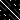
\includegraphics[width=4cm]{shearlets/inp_original}};
		\node at (4.4, 0) {
\includegraphics[width=4cm]{../scripts/p-learned}};
		\node at (4.4, -6.7) {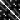
\includegraphics[width=4cm]{shearlets/inp_learned}};
		\begin{scope}[xshift=-2cm,yshift=-4.2cm]
			\begin{groupplot}[
				group style={
					group size=2 by 1,
					x descriptions at=edge bottom,
					y descriptions at=edge left,
					horizontal sep=4mm,
				},
				width=4cm,
				height=2cm,
				scale only axis,
			]
				\nextgroupplot
				\addplot [ycomb, mark=*] coordinates {%
					(1, 0.010493326175841)
					(2, -0.0263483047033631)
					(3, -0.051776695296637)
					(4, 0.276348304703363)
					(5, 0.582566738241592)
					(6, 0.276348304703363)
					(7, -0.0517766952966369)
					(8, -0.0263483047033631)
					(9, 0.0104933261758408)
				};
				\nextgroupplot
				\addplot [ycomb, mark=*] coordinates {%
					(1, 0.002334262477234006)
					(2, 0.017785610631108284)
					(3, -0.033911462873220444)
					(4, 0.04968487098813057)
					(5, 0.518813967704773)
					(6, 0.44657230377197266)
					(7, -0.0003913277178071439)
					(8, -0.013978870585560799)
					(9, 0.013090630993247032)
				};
			\end{groupplot}
		\end{scope}
	\end{tikzpicture}
	\caption[Initial and learned shearlets]{
		The first two rows show the two-dimensional directional filter \( P \) and the one-dimensional low-pass filter \( h \).
		The last row shows the cosine similarity of the magnitude of the spectra of the resulting shearlet system.
		A system exactly fulfilling the assumption~\eqref{eq:disjoint} would be unpopulated off the main diagonal.
	}
	\label{fig:shearlet building blocks}
\end{figure}
\begin{figure*}
	\begin{tikzpicture}
		\csvreader[no head]{chapters/regularizers/scripts/shearlets/lamdas.csv}{1=\llambda}{
			\pgfmathsetmacro{\component}{int(\thecsvrow-1)}
			\pgfmathsetmacro{\yy}{-int(\component/10)*1.6}
			\pgfmathsetmacro{\xx}{mod(\component,10)*1.6}
			\node at (\xx, \yy-.8) {\tiny \( \llambda \)};
			\node at (\xx, \yy+3.1) {\includegraphics[frame=3pt,width=1.3cm]{chapters/regularizers/scripts/shearlets/\component/sh_\component}};
			\node at (\xx, \yy) {\includegraphics[frame,width=1.3cm]{chapters/regularizers/scripts/shearlets/\component/k_\component}};
		}
		\draw [gray, thick, rounded corners] (-1.25cm, -2.6cm) rectangle (15.3cm, 4.0cm);
		\node at (-1.55cm, 0.5cm) [rotate=90] {Filters and spectra};
		\begin{scope}[xshift=-.65cm,yshift=-4.3cm]
			\begin{groupplot}[
				pogmdm group plot,
				group style={
					group size=10 by 2,
				},
				ymin=-1.5,
				ymax=3,
				width=1.3cm,
				height=1.3cm,
				xmin=-0.45,
				xmax=0.45,
				xticklabel=\empty,
			]
				\pgfplotsinvokeforeach{0,...,19}
				{%
					\nextgroupplot%
					\pgfplotsforeachungrouped \ccol in {a,b,c,d,e}
					{%
						\edef\tmp{%
							\noexpand\addplot table[col sep=comma, x=x, y=\ccol]{chapters/regularizers/scripts/shearlets/#1/potentials.csv};%
						}\tmp%
					}%
				}
			\end{groupplot}
			\draw [gray, thick, rounded corners] (-0.6cm, -1.8cm) rectangle (16.0cm, 1.5cm);
			\node at (-0.9cm, -0.15cm) [rotate=90] {Potentials};
		\end{scope}
		\begin{scope}[xshift=-.65cm,yshift=-7.8cm]
			\begin{groupplot}[
				pogmdm group plot,
				group style={
					group size=10 by 2,
				},
				ymin=-18,
				ymax=18,
				width=1.3cm,
				height=1.3cm,
				xmin=-0.45,
				xmax=0.45,
				xticklabel=\empty,
			]
				\pgfplotsinvokeforeach{0,...,19}
				{%
					\nextgroupplot%
					% Dummy plot to skip first entry in cycle list, since we don't want the gradient at 0 to show up as it is too noisy
					% probably there exist more elegant solutions
					\addplot {-1000};
					% Start at b to skip gradient at 0
					\pgfplotsforeachungrouped \ccol in {b,c,d,e}
					{%
						\edef\tmp{%
							\noexpand\addplot table[col sep=comma, x=x, y=\ccol]{chapters/regularizers/scripts/shearlets/#1/potentials-prime.csv};%
						}\tmp%
					}%
				}
			\end{groupplot}
			\draw [gray, thick, rounded corners] (-0.6cm, -1.8cm) rectangle (16.0cm, 1.5cm);
			\node at (-0.9cm, -0.15cm) [rotate=90] {Activations};
		\end{scope}
		\begin{scope}[xshift=-.65cm,yshift=-11.3cm]
			\begin{groupplot}[
				pogmdm group plot,
				group style={
					group size=10 by 2,
				},
				width=1.3cm,
				height=1.3cm,
				ymin=-17,
				ymax=0,
				xmin=-0.45,
				xmax=0.45,
				xtick={-0.4,-0.2,0,0.2,0.4},
				xticklabels={-0.4,,0,,0.4},
			]
				\pgfplotsinvokeforeach{0,...,19}
				{%
					\nextgroupplot%
					\pgfplotsforeachungrouped \ccol in {a,b,c,d,e}
					{%
						\edef\tmp{%
							\noexpand\addplot table[col sep=comma, x=x, y=\ccol]{chapters/regularizers/scripts/shearlets/#1/hists.csv};%
						}\tmp%
					}%
				}
			\end{groupplot}
			\draw [gray, thick, rounded corners] (-0.6cm, -2.1cm) rectangle (16.0cm, 1.5cm);
			\node at (-0.9cm, -0.3cm) [rotate=90] {Empirical marginals};
		\end{scope}
	\end{tikzpicture}
	\caption[Learned directions and potential functions]{%
		The learned overcomplete model utilizing Gaussian mixture expters.
		Below each filter its associated weight is shown.
		The learned potential functions (middle) are distinctly different from the negative-log empirical marginals (bottom).
		In particular, they have multiple local minima such that they can enhance certain structures.
		Sometimes (e.g. the second potential function from the left) zero is not even in the set of minima.
		The rows alternate between horizontal and vertical cones, and in reach row the first five plots show the five different shearings for the coarse detail level, \( j = \num{1} \) and the last five plots show the five different shearings for the finer detail level, \( j = \num{2} \).
		\tikzexternaldisable%
		The colors indicate the diffusion time \( \sqrt{\num{2}t} = %
			\num{0} \protect\tikz[baseline=-\the\dimexpr\fontdimen22\textfont2\relax]\protect\draw [index of colormap={0} of flare, thick] (0,0) -- (.5, 0); ,
			\num{0.025} \protect\tikz[baseline=-\the\dimexpr\fontdimen22\textfont2\relax]\protect\draw [index of colormap={4} of flare, thick] (0,0) -- (.5, 0); ,
			\num{0.05} \protect\tikz[baseline=-\the\dimexpr\fontdimen22\textfont2\relax]\protect\draw [index of colormap={8} of flare, thick] (0,0) -- (.5, 0); ,
			\num{0.1} \protect\tikz[baseline=-\the\dimexpr\fontdimen22\textfont2\relax]\protect\draw [index of colormap={12} of flare, thick] (0,0) -- (.5, 0); ,
			\num{0.2} \protect\tikz[baseline=-\the\dimexpr\fontdimen22\textfont2\relax]\protect\draw [index of colormap={17} of flare, thick] (0,0) -- (.5, 0);.
			\)
		\tikzexternalenable
	}%
	\label{fig:learned overcomplete regularizer}
\end{figure*}

We show the initial and learned the one-dimensional low-pass filter \( h_{\num{1}} \), and the two-dimensional directional filter \( P \) in~\cref{fig:shearlet building blocks} and the resulting shearlet system in frequency- and time-domain along with the learned experts in~\cref{fig:learned overcomplete regularizer}.
There, the rows alternate between horizontal and vertical cones, and in reach row the first five plots show the five different shearings for the coarse detail level, \( j = \num{1} \) and the last five plots show the five different shearings for the finer detail level, \( j = \num{2} \).
We again emphasize that the learned one-dimensional experts \( \Expert_{j,k,l}(\argm, w_{j,k,l}, t) \) are distinctly different from the other models.
In particular, the potentials \( - \log \psi_{j,k,l}(\argm, w_{j,k,l}, t) \) exhibit multiple local minima, sometimes different from \( \num{0} \), such that certain image structures can be enhanced under this prior.
This is in stark contrast to the learned filter- and wavelet-responses, which show a single minimum at \( \num{0} \) and the classical heavy-tailed shape.

Visual inspection of the spectra shown in \cref{fig:learned overcomplete regularizer} immediately reveals that the shearlet system only approximately fulfills the assumption~\eqref{eq:disjoint} and~\eqref{eq:constant}.
We analyze the shearlet system with respect to the assumption of disjoint support~\eqref{eq:disjoint} by visualizing the pair-wise cosine similarity of the magnitude of the spectra in~\cref{fig:shearlet building blocks}.
In detail, the figure shows \( \bigl\langle \frac{|\gamma_{\tilde{\jmath},\tilde{k},\tilde{l}}|}{\norm{\,|\gamma_{\tilde{\jmath},\tilde{k},\tilde{l}}|\,}}, \frac{|\gamma_{j,k,l}|}{\norm{\,|\gamma_{j,k,l}|\,}} \bigr\rangle \), for \( \tilde{\jmath}, j = \num{1}, \num{2} \), \( \tilde{k}, k = -\num{2}, \dotsc, \num{2} \) and \( \tilde{l}, l = \text{horizontal}, \text{vertical} \).\footnote{the exact arrangement irrelevant}
Although less for the learned shearlet system, the plot is dominated by the main diagonal, indicating that the corresponding spectra are almost non-overlapping.
To meet the theoretical assumptions, it would be possible to penalize \( \bigl\langle \frac{|\gamma_{\tilde{\jmath},\tilde{k},\tilde{l}}|}{\norm{\,|\gamma_{\tilde{\jmath},\tilde{k},\tilde{l}}|\,}}, \frac{|\gamma_{j,k,l}|}{\norm{\,|\gamma_{j,k,l}|\,}} \bigr\rangle \) for  \( \tilde\jmath \neq j \), \( \tilde{k} \neq k \), and \( \tilde{l} \neq l \) during training.

The fact that the spectra are not constant over their support raises the question of how to choose \( \xi_{j,k,l} \) that best approximates~\eqref{eq:constant}.
During training and evaluation, we simply chose \( \xi_{j,k,l} = \norm{\,|\gamma_{j,k,l}|\,}_\infty \).
It remains an open question how the violation of the constraints~\eqref{eq:disjoint} and ~\eqref{eq:constant} influences the diffusion, and if there exists a better choice for \( \xi_{j,k,l} \).
\subsection{Image denoising}
This section addresses the prototypical image restoration problem: image denoising.
To utilize the undercomplete model for image denoising, we employ the expected patch log-likelihood~\cite{zoran_learning_2011}.
Assuming that \( \UndercompleteModel(\argm, t) \) models the distribution of \( b \times b \) image patches, we define the expected patch log-likelihood of a noisy image \( y \in \R^{\Height\times\Width} \) with variance \( \sigma^{\num{2}}(t) = \num{2}t \) as
\begin{equation}
	\EPLL(y, t) = \sum_{i,j=\tilde{b}}^{\Height-\tilde{b},\Width - \tilde{b}} p_{i,j}^{-1} \log \UndercompleteModel(P_{i, j} y, t),
\end{equation}
where \( \tilde{b} = \lfloor b / \num{2} \rfloor \).
The sum ranges over all \emph{overlapping} patches, with \( \map{P_{i,j}}{\R^{\Height\times\Width}}{\R^{b\times b}} \) extracting the \( b \times b \) image patch centered at \( (i, j) \) and \( p_{i, j} = \bigl(\sum_{k,l=\tilde{b}}^{m-\tilde{b}, n-\tilde{b}} \Adjoint{P_{k,l}} P_{k,l} \mathbf{1} \bigr)_{i, j} \) counts the number of overlapping patches at \( (i, j) \) to compensate for boundary effects.\footnote{%
	Here, \( \mathbf{1} \) is the one-image in \( \R^{\Height\times\Width} \).
}
An example is illustrated in~\cref{fig:patch extraction}.
\begin{figure*}
	\begin{tikzpicture}[
		every node/.style={anchor=center,inner sep=0, thick, draw, minimum size=5mm},
		row 3 column 2/.style={draw=maincolor, thick},
		row 3 column 3/.style={draw=maincolor, thick},
		row 3 column 4/.style={draw=maincolor, thick},
		row 4 column 2/.style={draw=maincolor, thick},
		row 4 column 3/.style={draw=maincolor, thick},
		row 4 column 4/.style={draw=maincolor, thick},
		row 5 column 2/.style={draw=maincolor, thick},
		row 5 column 3/.style={draw=maincolor, thick},
		row 5 column 4/.style={draw=maincolor, thick},
	]
		\matrix (input) [matrix of nodes,column sep=0mm,row sep=0mm]
		{
			8 & 1 & 6 & 8 & 1 & 1 & 3 \\
			3 & 5 & 7 & 9 & 6 & 5 & 6 \\
			4 & 9 & 2 & 5 & 2 & 3 & 1 \\
			9 & 4 & 5 & 6 & 5 & 8 & 3 \\
			2 & 6 & 2 & 9 & 2 & 4 & 3 \\
			2 & 8 & 2 & 3 & 4 & 9 & 2 \\
		};
		\matrix (patch) at (4, 0) [matrix of nodes, nodes={draw=maincolor,}, column sep=0mm,row sep=0mm]
		{
			9 & 2 & 5 \\
			4 & 5 & 6 \\
			6 & 2 & 9 \\
		};
		\draw[-latex] (input-3-4) edge [out=40, in=130] node [draw=none, midway, above right] {\( P_{\num{4},\num{3}} \)} (patch) ;
		\matrix (output) at (8, 0) [matrix of nodes,column sep=0mm,row sep=0mm]
		{
			0 & 0 & 0 & 0 & 0 & 0 & 0 \\
			0 & 0 & 0 & 0 & 0 & 0 & 0 \\
			0 & 9 & 2 & 5 & 0 & 0 & 0 \\
			0 & 4 & 5 & 6 & 0 & 0 & 0 \\
			0 & 6 & 2 & 9 & 0 & 0 & 0 \\
			0 & 0 & 0 & 0 & 0 & 0 & 0 \\
		};
	\draw[-latex] (patch) edge [out=40, in=130]node [draw=none, midway, above] {\( \Adjoint{P_{\num{4},\num{3}}} \)} (output-3-2) ;

		\draw [ultra thick] (10.5, 1.8) -- ++(0, -3.6);
		\matrix (output) at (13, 0) [
		row 3 column 2/.style={draw=black, thick},
		row 3 column 3/.style={draw=black, thick},
		row 3 column 4/.style={draw=black, thick},
		row 4 column 2/.style={draw=black, thick},
		row 4 column 3/.style={draw=black, thick},
		row 4 column 4/.style={draw=black, thick},
		row 5 column 2/.style={draw=black, thick},
		row 5 column 3/.style={draw=black, thick},
		row 5 column 4/.style={draw=black, thick},
		matrix of nodes, column sep=0mm,row sep=0mm]
		{
			1 & 2 & 3 & 3 & 3 & 2 & 1 \\
			2 & 4 & 6 & 6 & 6 & 4 & 2 \\
			3 & 6 & 9 & 9 & 9 & 6 & 3 \\
			3 & 6 & 9 & 9 & 9 & 6 & 3 \\
			2 & 4 & 6 & 6 & 6 & 4 & 2 \\
			1 & 2 & 3 & 3 & 3 & 2 & 1 \\
		};
	\end{tikzpicture}
	\caption[Patch extraction operators and overlapping patches]{%
		\( P_{i,j} \) extracts a patch at pixel location \( (i, j) \), the adjoint \( \Adjoint{P_{i, j}} \) operator puts the patch into the corresponding location in a zero-image.
		On the right, the number of overlapping patches at each pixel location is shown.
		In the example, we consider a \numproduct{6x7} image and \numproduct{3x3} patches.
	}%
	\label{fig:patch extraction}
\end{figure*}
Wavelet- and shearlet-based priors can act on images of arbitrary size.

Let \( \log \GenericModel \) represent either \( \EPLL \), \( \log \WaveletModel \), or \( \log \OvercompleteModel \).
We consider three inference methods:
In the classical variational formulation
\begin{equation}
	\min_{x\in\R^{\Height\times\Width}} \Half \norm{x - y}^{\num{2}} - \lambda \log \GenericModel(x, t),
	\label{eq:pogmdm optim denoising}
\end{equation}
different choices of \( t > \num{0} \) are possible.
\( \log \GenericModel(\argm, t) \) approaching \( \DensityFunctionX \) as \( t \) approaches \num{0} motivates choosing \( t \) small.
However, smaller \( t \) make optimizing~\cref{eq:pogmdm optim denoising} more challenging as.
We chose \( t = \num{0.01} \) balancing optimization feasibility with model performance.

The empirical Bayes estimate
\begin{equation}
	\hat{x}_{\mathrm{EB}}(y, t) = y + \sigma^{\num{2}}(t) \Grad_{\num{1}} \log \GenericModel(y, t),
\end{equation}
is the most natural inference strategy in the context of this chapter.
This estimator provides the Bayesian \gls{mmse} through one gradient evaluation.
For the undercomplete model, \( \log \GenericModel = \EPLL \), the estimator
\begin{equation}
	\begin{aligned}
		\hat{x}_{\mathrm{EB}}(y, t) &= y + \sigma^{\num{2}}(t) \Grad_{\num{1}} \operatorname{epll}_\theta^{\mathrm{filt}}(y, t) \\
									&= y + \num{2}t \sum_{i,j=\tilde{b}}^{m-\tilde{b},n-\tilde{b}} p_{i,j}^{-1} \Adjoint{P_{i,j}} \Grad_{\num{1}} \log \UndercompleteModel(P_{i,j} y, t)
	\end{aligned}
	\label{eq:ebpa}
\end{equation}
computes patch-wise \gls{mmse} estimates and combines them by averaging.
This is known to be a sub-optimal inference strategy, since the averaged patches are not necessarily likely under the model~\cite{zoran_learning_2011}.
We refer the interested reader to the works of~\cite{romano_boosting_2017,zoran_learning_2011} for a detailed discussion on utilizing patch-based priors for whole-image restoration.

Lastly, we use recently proposed algorithms for inverse problems that utilize diffusion models.
We consider the stochastic denoising algorithm by~\cite{kawar_stochastic_2021} (see \cref{alg:stochastic image denoiser}) with standard parameters \( \epsilon = \num{5e-6} \), \( \sigma_{C} = \num{0.01} \) and the exponential schedule \( \sigma_i = \sqrt{\num{2}t} \bigl(\frac{\sigma_{C}}{\sqrt{\num{2}t}}\bigr)^{i/C} \), using \( B = \num{3} \) inner loops and \( C = \num{100} \) diffusion steps.
The algorithm samples from the posterior of a denoising problem when utilizing diffusion priors, effectively balancing the prior \( \Grad \log \GenericModel(\argm, t) \) and the data term as \( t \) approaches \( \num{0} \).
Sampling from the posterior often produce sharper results with modern diffusion models~\cite{Karras2022edm,kawar_stochastic_2021}.
\begin{algorithm}[t]
	\DontPrintSemicolon%
	\SetKwInOut{Output}{Output}
	\SetKwInOut{Input}{Input}
	\Input{Variance schedule \( \{ \sigma_i \}_{i=\num{1}}^C \), noisy image \( y \in \R^{\Height\times\Width} \), inner iterations \( B \in \mathbb{N} \), noise level \( \sigma_{\num{0}} \) in \( y \)}
	\Output{Stochastically denoised image \( x_B \)}
	\For{\( i \in \num{1}, \num{2}, \dotsc, C \)}{
		\(\alpha_i \leftarrow \epsilon \sigma_i^{\num{2}} / \sigma_{C}^{\num{2}} \)\;
		\For{\( b \in \num{1}, \dotsc, B - \num{1} \)}{
			\(z_b \sim \NormalDistribution_{\num{0}, \Identity} \)\;
			\(g_b \leftarrow \nabla \log \GenericModel(x_{b-\num{1}}, \sigma_i) + (y - x_{b-\num{1}}) / (\sigma_{\num{0}}^{\num{2}} - \sigma_i^{\num{2}}) \)\;
			\(x_b \leftarrow x_{b-\num{1}} + \alpha_i g_b + \sqrt{\num{2}\alpha_i}z_b\)\;
		}
		\( x_{\num{0}} \leftarrow x_B \)\;
	}
	\caption{%
		Stochastic image denoising algorithm from~\cite{kawar_stochastic_2021}.
	}%
	\label{alg:stochastic image denoiser}
\end{algorithm}

\Cref{tab:denosing} shows quantitative results using \gls{psnr} (\cref{def:psnr}) and \gls{ssim} (\cref{def:ssim}), computed with a uniform \numproduct{7x7} filter and parameters \( K_{\num{1}} = \num{0.01} \) and \( K_{\num{2}} = \num{0.03} \).
The column titled \enquote{Patch-\glsxtrshort{gsm}} utilizes the Gaussian scale mixture parametrization discussed in~\cref{ssec:alternative parametrizations}.
The results are for one run of the algorithms without computing the expectation over the noise (neither in the construction of \( y_t \) nor during the iterations of the stochastic denoising algorithm), thus confidence intervals reflect only image variability in the test dataset.
We do not discuss posterior variance in this chapter but techniques for analyzing the posterior induced by diffusion models are also readily applicable to our models.
We refer to~\cite{kawar_stochastic_2021} or related papers such as~\cite{chung2023diffusion} for an in-depth discussion of these techniques.

For the variational formulation, the overcomplete model performs best when the noise level is small.
However, the undercomplete model with \gls{gsm} experts surpasses other models at high noise levels dur to its smooth, non-oscillatory tails.
While the models are trained to approximate the reference density \( \DensityFunctionX \) at time \num{0}, the potentials become oscillatory in practice.
Oscillatory potentials, as seen in the wavelet model (see \cref{fig:learned wavelet regularizer}), hinder optimization, but \gls{gsm} experts' smooth tails avoid this issue.\footnote{
	However, \glspl{gsm} cannot represent multi-modal densities like \glspl{gmm}.
}

The oscillation problem can be mitigated by considering a decreasing time sequence and optimizing the variational objective, where subsequent problems are initialized with previous solutions.
This has strong relations to classical continuation methods used in computer vision, see e.g.~\cite{Witkin1987,Yuille1989}.
A proximal-gradient continuation method is presented in our preliminary work~\cite{zach_explicit_2023}.
Kobler and Pock's joint minimization approach using preconditioned proximal-gradient~\cite[figure 4]{kobler2023learning} also shows promising results.
In addition, they show that \emph{learning} a decreasing time sequence and step sizes of an optimization algorithm improves the results, which is is strongly related to variational networks.
However, in their approach only the \enquote{parameters} of the optimization algorithm are learned whereas the model remains fixed.

The empirical Bayes estimator demonstrates the overcomplete model's parameter efficiency, performing close to \gls{gmm}-\gls{epll}~\cite{zoran_learning_2011} with significantly fewer parameters.
\emph{One} full covariance matrix on \( \R^{\numproduct{7x7}} \) has \num{1226} learnable parameters, slightly less than the \num{1642} parameters in our overcomplete model.
With one component, \gls{gmm}-\gls{epll} effectively reduces to quadratic potentials acting on filter responses, which is a bad model for natural images (see \cref{chap:regularizers}).
Thus, we use the setup of the original paper~\cite{zoran_learning_2011} with \num{200} components, totaling \( \num{200} (\num{1} + \num{49} + \num{49}\ \text{choose}\ \num{2}) = \num{245200} \) learnable parameters.
Leveraging symmetries in the shearlet system could increase parameter efficiency further:
Sharing the potentials between the cones would half the number of parameters (the symmetry is apparent in \cref{fig:learned overcomplete regularizer}).

The overcomplete model's performance deteriorates with higher noise levels, likely due to a mismatch between theoretical filter assumptions and the practical shearlet characteristics.
Specifically, the magnitude of the spectra is only approximately constant on the support and we adapting the variances with the maximum may not be the optimal choice.

The empirical Bayes estimator outperforms stochastic denoising in all quality metrics, likely because only one sample is drawn in the stochastic algorithm;
multiple samples would likely improve quantitative results.
The empirical Bayes estimator consistently beats the variational approach only for the overcomplete model.
The undercomplete models appear to be better suited for \gls{map} estimation than \gls{mmse} estimation, highlighting the difference between penalized likelihood estimation and Bayesian estimation:
good results in \gls{map} estimation can occur even with a poor prior model\footnote{%
	The most prominent example is image restoration with total variation penalization.
}
Conversely, Nikolova~\cite{nikolova2007model} and Schmidt et al.~\cite[section 5]{schmidt_generative_2010} point out that good prior models are not well suited for \gls{map} estimation.

Qualitative results using the variational approach, empirical Bayes estimation, and stochastic denoising are shown in~\cref{fig:denoising optimization},~\cref{fig:denoising empirical bayes}, and~\cref{fig:denoising stochastic}, respectively.
The overcomplete model produces more natural reconstructions particularly with Empirical Bayes estimation.
Prominent structures, like the tiger stripes, are sometimes emphasized due to complex learned potentials.
In contrast, the reconstructions of the undercomplete models appear overly smooth, removing rather than enhancing structures.
Surprisingly, sharper images were not observed with the stochastic denoising algorithm.
% https://tex.stackexchange.com/questions/19017/how-to-place-a-table-on-a-new-page-with-landscape-orientation-without-clearing-t?noredirect=1&lq=1
% I had to put restoregeometry outside of the afterpage though, otherwise the text on the next page runs off
\afterpage{%
\clearpage%
\thispagestyle{empty}%
\newgeometry{left=1cm,right=2cm,bottom=2cm,top=2cm}%
\begin{landscape}
	\centering
	\begin{tabular}{%
		cc%
		S[table-format=1.3]%
		*{8}{S[table-format=2.2(1),separate-uncertainty=true,retain-zero-uncertainty,table-align-uncertainty]}
	}
		\toprule
		& & {\multirow{2}{*}{\( \sigma \)}} & {\multirow{2}{*}{\( y_t \)}} & \multicolumn{2}{c}{{Patch-GMM}} & {-GSM} & \multicolumn{2}{c}{{Wavelet}} & {\multirow{2}{*}{Shearlet}} & {\multirow{2}{*}{\glsxtrshort{tv}}} \\\cmidrule(l{1em}r{1em}){5-6}\cmidrule(l{1em}r{1em}){8-9}
		& & & & {\( b = \num{7} \)} & {\( b = \num{15} \)} & {\( b = \num{7} \)} & {\( K = \num{4} \)} & {\( K = \num{8} \)} & & \\
		\midrule
		\multirow{8}{*}{\rotatebox[origin=c]{90}{Optimization}} & \multirow{4}{*}{\rotatebox[origin=c]{90}{\gls{psnr}}} & 
		0.025 & 32.04(00) & 34.70(29) & 35.17(29) & 35.41(35) & 33.67(28) & 33.74(30) & \bfseries 34.98(31) & 34.63(34) \\
  & & 0.050 & 26.02(00)  &  29.90(55) & 30.91(35) & 31.26(42) & 29.12(42) & 29.03(31) & \bfseries 30.88(46) & 30.42(38) \\
  & & 0.100 & 20.00(00)  &  27.29(44) & 27.70(55) & \bfseries 27.94(53) & 24.09(27) & 23.96(25) & 27.03(57) & 27.12(54) \\
  & & 0.200 & 13.98(00)  & 24.46(46) &  24.91(56) & \bfseries 24.99(61) & 18.43(13) & 18.42(12) & 18.03(12) & 24.25(66) \\
		\cmidrule{2-11}
		& \multirow{4}{*}{\rotatebox[origin=c]{90}{\gls{ssim}}} &
		0.025 & 0.84(02) & 0.93(01) & \bfseries 0.94(00) & \bfseries 0.94(00) & 0.91(01) & 0.91(01) & \bfseries 0.94(00) & 0.93(00) \\
  & & 0.050 & 0.65(03) &   0.85(01) & 0.86(01) & \bfseries 0.88(01) & 0.81(01) & 0.79(01) & 0.87(01) & 0.85(01) \\
  & & 0.100 & 0.41(03) &   0.74(01) & 0.78(01) & \bfseries 0.79(01) & 0.56(02) & 0.56(02) & 0.76(02) & 0.75(01) \\
  & & 0.200 & 0.21(02) &   0.61(01) & \bfseries 0.66(02) & \bfseries 0.66(02) & 0.30(02) & 0.30(02) & 0.34(02) & 0.62(03) \\
		\midrule
  & & & & & & & & & & {GMM-EPLL} \\\midrule
		\multirow{8}{*}{\rotatebox[origin=c]{90}{Empirical Bayes}} & \multirow{4}{*}{\rotatebox[origin=c]{90}{\gls{psnr}}} & 
		0.025 & 32.04(00) & 34.54(21) & 35.00(27) & 35.08(29) & 33.51(23) & 33.61(25) & 35.30(38) & \bfseries 35.59(35) \\
			  & & 0.050 & 26.02(00)  & 30.44(32) & 30.79(37) & 30.80(37) & 29.32(29) & 29.48(31) & 31.17(44) & \bfseries 31.68(46) \\
			  & & 0.100 & 20.00(00)  & 27.03(42) & 27.27(46) & 27.20(44) & 25.72(36) & 25.90(36) & 27.50(46) & \bfseries 28.12(50) \\
			  & & 0.200 & 13.98(00)  & 24.24(48) & 24.45(52) & 24.29(48) & 22.41(33) & 22.54(32) & 23.91(40) & \bfseries 24.92(51)\\
		\cmidrule{2-11}
		& \multirow{4}{*}{\rotatebox[origin=c]{90}{\gls{ssim}}} &
		0.025 & 0.84(02) & 0.92(01) & 0.93(01) & 0.93(00) & 0.90(01) & 0.90(01) & 0.94(00) & \bfseries 0.95(00) \\
			  & & 0.050 & 0.65(03) & 0.83(01) & 0.85(01) & 0.85(01) & 0.80(01) & 0.80(01) & 0.87(01) & \bfseries 0.89(01) \\
			  & & 0.100 & 0.41(03) & 0.72(01) & 0.73(01) & 0.73(01) & 0.65(02) & 0.66(02) & 0.75(01) & \bfseries 0.79(01)\\
			  & & 0.200 & 0.21(02) & 0.58(01) & 0.60(01) & 0.59(01) & 0.48(02) & 0.49(02) & 0.55(01) & \bfseries 0.63(01)\\
		\midrule
		\multirow{8}{*}{\rotatebox[origin=c]{90}{Stochastic Denoising}}&\multirow{4}{*}{\rotatebox[origin=c]{90}{\gls{psnr}}} &
		0.025 & 32.04(00) & 31.34(11) & 31.79(16) & 31.88(18) & 30.68(10) & 30.78(11) & \bfseries 32.40(27) & {---} \\
			  & & 0.050 & 26.02(00) & 27.07(18) & 27.55(23) & 27.62(25) & 26.00(14) & 26.17(15) & \bfseries 28.46(40) & {---} \\
			  & & 0.100 & 20.00(00) & 23.66(24) & 24.06(27) & 24.06(28) & 22.03(15) & 22.24(16) & \bfseries 24.94(44) & {---} \\
			  & & 0.200 & 13.98(00) & 20.90(25) & \bfseries 21.24(29) & 21.12(28) & 18.60(13) & 18.71(13) & 21.10(34) & {---} \\
		\cmidrule{2-11}
		& \multirow{4}{*}{\rotatebox[origin=c]{90}{\gls{ssim}}} &
		0.025 & 0.84(02) & 0.84(02) & 0.85(01) & 0.86(01) & 0.82(02) & 0.82(02) & \bfseries 0.88(01) & {---}  \\
			  & & 0.050 & 0.65(03) & 0.69(02) & 0.71(02) & 0.72(02) & 0.65(02) & 0.65(02) & \bfseries 0.78(01) & {---} \\
			  & & 0.100 & 0.41(03) & 0.52(02) & 0.54(02) & 0.54(02) & 0.46(03) & 0.47(03) & \bfseries 0.63(01) & {---} \\
			  & & 0.200 & 0.21(02) & 0.36(02) & 0.37(02) & 0.37(02) & 0.29(02) & 0.30(02) & \bfseries 0.41(01) & {---} \\
		\midrule
			  \multicolumn{4}{c}{Learnable parameters} & {\num{5376}} & {\num{78400}} & {\num{3312}} & {\num{389}} & {\num{393}} & {\num{1642}} & {\num{245200}} \\\bottomrule
	\end{tabular}
	\captionof{table}[Quantitative denoising results]{%
		Quantitative results in terms of \glsxtrshort{psnr} and \glsxtrshort{ssim} using one-step empirical Bayes denoising the stochastic denoising algorithm from~\cite{kawar_stochastic_2021}.
		The intervals indicate the \num{0.95} confidence region, bold typeface indicates the best method.
	}%
	\label{tab:denosing}
\end{landscape}%
\clearpage%
}
\restoregeometry%
\def\spyxoff{-1mm}
\def\spyyoff{-1mm}
\begin{figure*}
	\centering
	\begin{tikzpicture}
		\foreach [count=\isigma] \ssigma in {0.025, 0.050, 0.100, 0.200} {
			\pgfmathsetlengthmacro{\yy}{-\isigma * (\wwidth + \wwidth / 2 + \vpad)}
			\foreach [count=\imethod] \mmethod/\manno in {
				gmm7/{GMM, \( b = \num{7} \)},
				gmm15/{\( b = \num{15} \)},
				gsm7/{GSM, \( b = \num{7} \)},
				wavelet-db4/{Wavelet, \( K = \num{8} \)},
				shearlet/{Shearlet},
				tv/{TV}%
			}{
				\pgfmathsetlengthmacro{\xx}{\imethod * (\wwidth + \hpad)}
				\ifthenelse{\isigma=1}{\node at (\xx, -\wwidth / 2 - 1cm) {\manno};}{}
				\coordinate (onn) at (\xx + \spyxoff, \yy + \spyyoff);
				\begin{scope}[mrispy]
					\node[inner sep=0, outer sep=0] at (\xx, \yy) {\includegraphics[width=\wwidth]{denoising/optim/\ssigma/\mmethod/006_d}};
					\spy on (onn) in node at (\xx + \wwidth / 2 / 2, \yy - 1.5 * \wwidth / 2);
				\end{scope}
				\begin{scope}[mrispy]
					\node[inner sep=0, outer sep=0] at (\xx, \yy) {\includegraphics[width=\wwidth]{denoising/optim/\ssigma/\mmethod/006}};
					\spy on (onn) in node at (\xx - \wwidth / 2 / 2, \yy - 1.5 * \wwidth / 2);
				\end{scope}
			}
		}
	\end{tikzpicture}
	\caption[Qualitative results for optimization-based denoising]{%
		Qualitative results for optimization-based denoising.
		In the rows, the noise standard deviation ranges in \( \sigma \in \Set{ \num{0.025}, \num{0.05}, \num{0.1}, \num{0.2}} \).
		The inlays show a zoomed region (magnifying factor \num{3}), and the absolute difference of the reconstruction to the ground truth image (\num{0}~\protect\drawcolorbar~\(\num{1}/\num{3}\)).
		The accompanying quantitative results are shown in~\cref{tab:denosing}.
	}%
	\label{fig:denoising optimization}
\end{figure*}
\begin{figure*}
	\centering
	\begin{tikzpicture}
		\foreach [count=\isigma] \ssigma in {0.025, 0.050, 0.100, 0.200} {
			\pgfmathsetlengthmacro{\yy}{-\isigma * (\wwidth + \wwidth / 2 + \vpad)}
			\foreach [count=\imethod] \mmethod/\manno in {
				gmm7/{GMM, \( b = \num{7} \)},
				gmm15/{\( b = \num{15} \)},
				gsm7/{GSM, \( b = \num{7} \)},
				wavelet-db4/{Wavelet, \( K = \num{8} \)},
				shearlet/{Shearlet},
				gmm-epll/{GMM-EPLL}%
			}{
				\pgfmathsetlengthmacro{\xx}{\imethod * (\wwidth + \hpad)}
				\ifthenelse{\isigma=1}{\node at (\xx, -\wwidth / 2 - 1cm) {\manno};}{}
				\coordinate (onn) at (\xx + \spyxoff, \yy + \spyyoff);
				\begin{scope}[mrispy]
					\node[inner sep=0, outer sep=0] at (\xx, \yy) {\includegraphics[width=\wwidth]{denoising/tweedie/\ssigma/\mmethod/006_d}};
					\spy on (onn) in node at (\xx + \wwidth / 2 / 2, \yy - 1.5 * \wwidth / 2);
				\end{scope}
				\begin{scope}[mrispy]
					\node[inner sep=0, outer sep=0] at (\xx, \yy) {\includegraphics[width=\wwidth]{denoising/tweedie/\ssigma/\mmethod/006}};
					\spy on (onn) in node at (\xx - \wwidth / 2 / 2, \yy - 1.5 * \wwidth / 2);
				\end{scope}
			}
		}
	\end{tikzpicture}
	\caption[Qualitative results for one-step empirical bayes denoising]{%
		Qualitative results for one-step empirical Bayes denoising.
		In the rows, the noise standard deviation ranges in \( \sigma \in \Set{ \num{0.025}, \num{0.05}, \num{0.1}, \num{0.2}} \).
		The inlays show a zoomed region (magnifying factor \num{3}), and the absolute difference of the reconstruction to the ground truth image (\num{0}~\protect\drawcolorbar~\(\num{1}/\num{3}\)).
		The accompanying quantitative results are shown in~\cref{tab:denosing}.
	}%
	\label{fig:denoising empirical bayes}
\end{figure*}
\begin{figure*}
	\centering
	\begin{tikzpicture}
		\foreach [count=\isigma] \ssigma in {0.025, 0.050, 0.100, 0.200} {
			\pgfmathsetlengthmacro{\yy}{-\isigma * (\wwidth + \wwidth / 2 + \vpad)}
			\foreach [count=\imethod] \mmethod/\manno in {
				noisy/{\( y_t \)},
				gmm7/{\gls{gmm}, \( b = \num{7} \)},
				gmm15/{\( b = \num{15} \)},
				gsm7/{\gls{gsm}, \( b = \num{7} \)},
				wavelet-db4/{Wavelet, \( K = \num{8} \)},
				shearlet/{Shearlet}
			}{
				\pgfmathsetlengthmacro{\xx}{\imethod * (\wwidth + \hpad)}
				\ifthenelse{\isigma=1}{\node at (\xx, -\wwidth / 2 - 1cm) {\manno};}{}
				\coordinate (onn) at (\xx + \spyxoff, \yy + \spyyoff);
				\begin{scope}[mrispy]
					\node[inner sep=0, outer sep=0] at (\xx, \yy) {\includegraphics[width=\wwidth]{denoising/stoch/\ssigma/\mmethod/006_d}};
					\spy on (onn) in node at (\xx + \wwidth / 2 / 2, \yy - 1.5 * \wwidth / 2);
				\end{scope}
				\begin{scope}[mrispy]
					\node[inner sep=0, outer sep=0] at (\xx, \yy) {\includegraphics[width=\wwidth]{denoising/stoch/\ssigma/\mmethod/006}};
					\spy on (onn) in node at (\xx - \wwidth / 2 / 2, \yy - 1.5 * \wwidth / 2);
				\end{scope}
			}
		}
	\end{tikzpicture}
	\caption[Qualitative results for stochastic denoising]{%
		Qualitative results using the stochastic denoising algorithm from~\cite{kawar_stochastic_2021}.
		In the rows, the noise standard deviation ranges in \( \sigma \in \Set{ \num{0.025}, \num{0.05}, \num{0.1}, \num{0.2}} \).
		The inlays show a zoomed region (magnifying factor \num{3}), and the absolute difference of the reconstruction to the reference image (\num{0}~\protect\drawcolorbar~\(\num{1}/\num{3}\)).
		The accompanying quantitative results are shown in~\cref{tab:denosing}.
	}%
	\label{fig:denoising stochastic}
\end{figure*}

\subsection{Noise estimation and blind image denoising}
Within this and the following subsection, we describe two applications that arise as a byproduct of our principled approach:
Noise estimation (and, consequently, blind denoising) and analytic sampling.
For both, we utilize the undercomplete model as a stand-in but we believe that generalizations to the overcomplete model are possible.

The construction of our model allows us to interpret \( \UndercompleteModel(\argm, t) \) as a time-conditional density.
Thus, it can naturally be used for noise level estimation:
Assume that a noisy image patch \( y \in \R^{b \times b} \) is constructed by \( y = x + \sigma \eta \), where \( x \sim \DensityFunctionX \), \( \eta \sim \NormalDistribution_{\num{0}, \Identity} \), and the noise level \( \sigma \) is unknown.
We can estimate the noise level by maximizing the likelihood of the given patch \( y \) w.r.t.\ to the diffusion time---\(\hat{t} = \argmax_t \UndercompleteModel(y, t) \)---and recover the noise level via \( \hat{\sigma} = \sqrt{\num{2}\hat{t}} \).

To demonstrate the feasibility of this approach, we show the expected negative-log density \( \mathbb{E}_{x \sim \DensityFunctionX, \eta \sim \NormalDistribution_{\num{0}, \Identity}} \bigl[ l_\theta(x + \sigma\eta, t) \bigr] \) over a range of \( \sigma \) and \( t \) in~\cref{fig:noise estimation}.
Here, for visualization purposes we normalized the negative-log density to have a minimum of zero over \( t \):
\begin{equation}
	l_\theta(x, t) = -\log \UndercompleteModel(x, t) - \bigl( \max_t \log \UndercompleteModel\theta(x, t) \bigr).
\end{equation}
The noise level estimate \( \sigma \mapsto \argmin_t \mathbb{E}_{x \sim p_X, \eta \sim \NormalDistribution_{\num{0}, \Identity}} \bigl[ l_\theta(x + \sigma\eta, t) \bigr] \) perfectly matches the identity map \( \sigma \mapsto \sqrt{\num{2}t} \).
\begin{sidefigure}
	\centering
	\begin{tikzpicture}
		\begin{axis}[ymax=2, width=3.5cm, scale only axis, height=3cm, xtick={0,0.1,0.2,0.3,0.4,0.5, 1}, xticklabels={0,,,,,0.5,1}]
			\pgfplotsforeachungrouped \ccol in {a,b,c,d}
			{%
				\edef\tmp{%
					\noexpand\addplot+ [thick] table[col sep=comma, x=x, y=\ccol]{chapters/pogmdm/figures/energy.csv};%
				}\tmp%
			}%
			\legend{$\sigma=\num{0.1}$,$\num{0.2}$,$\num{0.3}$,$\num{0.4}$}
		\end{axis}
	\end{tikzpicture}
	\caption[Noise estimation]{%
		Expected normalized negative log-density \( \sqrt{\num{2}t} \mapsto \mathbb{E}_{x \sim p_X, \eta \sim \NormalDistribution_{\num{0}, \Identity}} \bigl[ l_\theta(x + \sigma\eta, t) \bigr] \)  for different noise levels.
	}%
	\label{fig:noise estimation}
\end{sidefigure}

The previous result showed that the noise estimation works in expectation.
Now, we provide empirical evidence that the noise estimation is reasonably robust with respect to instances of the noise and the content of the underlying image.
To this end, we perform blind heteroscedastic denoising as follows:
First, for all overlapping patches \( P_{i, j} y \), \( i = \tilde{b}, \tilde{b} + \num{1}, \dotsc, m - \tilde{b} \), \( j = \tilde{b}, \tilde{b} + \num{1}, \dotsc, n - \tilde{b} \) in the noisy image, we optimize the diffusion time: \( \hat{t}_{i, j} = \argmax_t \UndercompleteModel(P_{i, j} y, t) \).
Then, given the diffusion times \( \hat{t}_{i, j} \), we can estimate the clean image via an empirical Bayes step of the form
\begin{equation}
	\hat{x}_{\mathrm{blind}}(y) = y + \num{2} \sum_{i,j=\tilde{b}}^{m-\tilde{b}, n - \tilde{b}} \hat{t}_{i, j}  p_{i, j}^{-1} \Adjoint{P_{i, j}} \Grad_{1} \log \UndercompleteModel(P_{i, j} y, \hat{t}_{i, j}),
	\label{eq:blind eb}
\end{equation}
where for each patch \( P_{i, j} y \) we utilize the estimated diffusion time \( \hat{t}_{i, j} \).

In the first column of~\cref{fig:blind denosing}, we show six images corrupted by heteroscedastic Gaussian noise, where the standard deviation alternates between \num{0.1} and \num{0.2} in a checkerboard pattern.
This checkerboard pattern is clearly visible in the visualization of the optimal diffusion time in the second column.
The restored image and the absolute difference to the reference image are shown in the third and fourth column.
There, the checkerboard pattern is hardly visible, indicating that the noise level estimation is robust also when confronted with little data.
\begin{figure*}
	\centering
	\begin{tikzpicture}
		\def\wwidth{3cm}
		\def\vsep{2mm}
		\def\hsep{1mm}
		\foreach [count=\imcount] \cherry/\rot in {1/-90, 2/-90, 3/0, 4/-90, 5/0, 6/0} {
			\pgfmathsetlengthmacro{\yy}{-\imcount*(\wwidth + \vsep)}
			\foreach [count=\ii] \wwhich in {noisy, estimate_padded, denoised, diff} {
				\pgfmathsetlengthmacro{\xx}{\ii * (\wwidth + 1cm + \hsep)}
				\begin{scope}[spy using outlines={rectangle, magnification=3, width=1.cm, height=3cm, connect spies}]
					\node[rotate=\rot] at (\xx, \yy) {\includegraphics[width=\wwidth]{blind/\cherry/\wwhich}};
					\spy on (\xx, \yy) in node at (\xx+2cm, \yy);
				\end{scope}
			}
		}
	\end{tikzpicture}%
	\caption[Noise estimation and blind denoising]{%
		Noise estimation and blind denoising:
		The columns show the input image corrupted with heteroscedastic Gaussian noise in a checkerboard pattern with standard deviation \num{0.1} and \num{0.2}, the patch-wise noise level estimate (\num{0}~\protect\drawcolorbarbw~\num{0.5}), the one-step empirical Bayes denoising result using~\eqref{eq:blind eb}, and its absolute difference to the reference image (\num{0}~\protect\drawcolorbar~\(\num{1}/\num{3}\)).
	}%
	\label{fig:blind denosing}
\end{figure*}

\subsection{Sampling}%
\label{ssec:sampling}
A direct consequence of~\cref{cor:marginal} is that the undercomplete model admits a simple sampling procedure:
The statistical independence of the components allows drawing random patches by
\begin{equation}
	Y_t = \sum_{k=\num{1}}^\NumExperts \frac{\Filter_k}{\norm{\Filter_k}^{\num{2}}} U_{k, t},
	\label{eq:analytic sampling}
\end{equation}
where \( U_{k, t} \) is a random variable on \( \R \) sampled from the one-dimensional expert \( \Expert_k(\argm, w_k, t) \).

In~\cref{fig:patch generation results}, we show samples from the reference distribution along with samples from the learned models where the experts are \glspl{gmm} or \glspl{gsm}.
In both cases, the generated patches appear slightly noisy for small \( t \).
This indicates that the parametrization is not \enquote{peaky enough} around \num{0}.
However, the discretization is easily adapted:
For the \gls{gmm}, the discretization of the means as equidistant over the real line could be changed to, e.g., a logarithmic scaling resulting in a denser grid around \num{0}.
This would require the base-variance \( \sigma_{\num{0}}^{\num{2}} \) to change with the mean, which is also possible in our model.
For the \gls{gsm}, the peakiness of the expert is determined by the smallest variance, which is entirely up to choice; see the discussion in~\cref{sec:discussion}.

We believe that the structure of the linear operators in the overcomplete models also allows for an efficient sampling procedure; this is subject to future work.
\begin{figure*}
	\centering
	\def\wwidth{3cm}
	\begin{tikzpicture}
		\foreach [count=\isigma] \ssigma/\llabel/\ccolor in {%
			0.000/0/coolwarm1,
			0.025/0.025/coolwarm2,
			0.050/0.05/coolwarm3,
			0.100/0.1/coolwarm4,
			0.200/0.2/coolwarm5%
		}{%
			\foreach [count=\iwhich] \which in {reference, gmm, gsm}{%
				\node at (\isigma*\wwidth+\isigma*4, -\iwhich*\wwidth-\iwhich*7) {\includegraphics[Clip={.5\width} {0\height} {0\width} {0\height}, width=\wwidth]{patch/sampling/\which/\ssigma.png}};
			}
			\node (anno\isigma) at (\isigma*\wwidth+\isigma*4, -1.5){\ifthenelse{\isigma=1}{\( \sqrt{\num{2}t} = \num{\llabel} \)}{\( \num{\llabel} \)}};
		}
	\end{tikzpicture}
	\caption[Reference and generated patches at different noise levels]{%
		Reference samples from the random variable \( Y_t \) (top) and samples generated by the analytic sampling procedure~\eqref{eq:analytic sampling} using \gls{gmm} experts (middle) and \gls{gsm} experts (bottom).
	}%
	\label{fig:patch generation results}
\end{figure*}
\section{Discussion}%
\label{sec:discussion pogmdm}
In this section, we first give an interpretation of our learned complete model in the wavelet basis as \emph{diffusion wavelet shrinkage}.
Then, we discuss possible extensions to our model in more detail:
Alternative parametrizations and the possibilities of building more expressive models.
Finally, we again highlight the difference of the undercomplete and the overcomplete model and the implication of overcompleteness.
\subsection{Interpretation as diffusion wavelet shrinkage}
Wavelet shrinkage is a popular class of denoising algorithms.
Starting from the seminal works of Donoho~\cite{donoho_denoising_1995,donoho_adapting_1995,donoho_ideal_1994}, a vast literature is dedicated to finding optimal shrinkage parameters for wavelet-based denoising (see, e.g.\ \cite{chambolle_nonlinear_1998,chipman_adaptive_1997,clyde_multiple_1998,crouse_wavelet-based_1998,JANSEN199733,simoncelli_noise_1996} and the references therein).
In what follows, we briefly describe  historical approaches to estimating shrinkage parameters.

The key motivation behind wavelet shrinkage denoising algorithms is the observation that wavelet coefficients of natural images are sparse, wheres the wavelet coefficients of noisy images are densely filled with \enquote{small} values.
Thus, a straight forward denoising algorithm might be to calculate the wavelet coefficients, \enquote{shrink} small coefficients towards zero, and calculate the inverse wavelet transform of the shrank coefficients.
In the terminology we use in this thesis, wavelet shrinkage algorithms \emph{penalized likelihood estimation} algorithms.
\begin{sidefigure}
	\centering
	\begin{tikzpicture}
		\begin{axis}[marginplot, samples=300, domain=-1:1, width=3.5cm, clip=false]
			\addplot+ [thick] {max(abs(x) - 0.5, 0) * sign(x)};
			\addplot+ [thick] {x * (abs(x) > 0.5)};
			\addplot+ [thick] table[col sep=comma, x=x, y=e]{chapters/regularizers/scripts/wavelets/db4/tweedie/1_1.csv};%
		\end{axis}
	\end{tikzpicture}
	\caption[Popular wavelet shrinkage functions]{%
		\tikzexternaldisable%
		Popular wavelet shrinkage functions: The soft-shrinkage %
		\protect\tikz[baseline=-\the\dimexpr\fontdimen22\textfont2\relax]\protect\draw [index of colormap={0} of flare, thick] (0,0) -- (.5, 0); and the hard-shrinkage 
		\protect\tikz[baseline=-\the\dimexpr\fontdimen22\textfont2\relax]\protect\draw [index of colormap={4} of flare, thick] (0,0) -- (.5, 0); with threshold parameter \( \tau = \num{0.5} \).
		In addition, the learned \gls{mmse} optimal shrinkage function
		\protect\tikz[baseline=-\the\dimexpr\fontdimen22\textfont2\relax]\protect\draw [index of colormap={8} of flare, thick] (0,0) -- (.5, 0);.
		\tikzexternalenable
	}%
	\label{fig:shrinkage functions}
\end{sidefigure}
Popular shrinkage operators include the soft-shrinkage%
\begin{equation}
	x \mapsto \operatorname{sgn}(x) \max(|x| - \tau, \num{0})
\end{equation}
and the hard-shrinkage
\begin{equation}
	x \mapsto x \CharacteristicFunction{\Set{y\in\R\given -\tau < y \leq \tau}}(x).
\end{equation}
It is easy to see that these operators promote sparsity in the wavelet coefficients, as they correspond to the proximal maps (\cref{def:proximal operator}) with respect to the sparsity inducing norms \( \tau\norm{\argm}_{\num{1}} \) and \( \tau\norm{\argm}_{\num{0}} \) respectively;
they are visualized in~\cref{fig:shrinkage functions}.
Here, \( \tau > \num{0} \) is a thresholding parameter that has to be chosen depending on the noise level.

Historically, research for wavelet shrinkage models has focused on finding the optimal shrinkage parameter \( \tau \) (w.r.t.\ some risk, e.g.\ the squared error), assuming a particular choice of the shrinkage operator (e.g.\ the soft-shrinkage).
Popular selection methods include \emph{VisuShrink}~\cite{donoho_ideal_1994} and \emph{SureShrink}~\cite{donoho_adapting_1995}.
The former is signal independent and the threshold is essentially determined by the dimensionality of the signal as well as the (assumed known) noise level.
In contrast, the latter chooses the thresholding parameter depending on the energy in a particular sub-band and does not depend on the dimensionality of the signal explicitly.
The \emph{BayesShrink}~\cite{chang_adaptive_2000} method is also sub-band adaptive, and the authors provide expressions (or at least good approximations) for the optimal thresholding parameter under a generalized Gaussian prior on the wavelet coefficients.
In particular, they rely on classical noise level estimation techniques to fit the generalized Gaussian to the wavelet coefficients (of the noisy image) and arrive at a simple expression for a sub-band dependent threshold.

The general methodology outlined in the previous section allows us to take a different approach:
Instead of fixing the thresholding function and estimating the threshold solely on the corrupted image, we instead propose to learn the distribution of wavelet coefficients in different sub-bands for all noise levels \( \sigma > \num{0} \).
Notice that an empirical Bayes step on the wavelet coefficients under our model corresponds to applying a point-wise non-linearity.

In contrast to the traditional wavelet shrinkage, our model does not prescribe a shrinkage function for which an optimal parameter has to be estimated for different noise levels.
Rather, by learning the distribution of the wavelet coefficients at \enquote{all} noise levels, we have access to an \gls{mmse} optimal \enquote{shrinkage} function view of the empirical Bayes step on the experts.
In addition, our wavelet prior can be used in more general inverse problems whereas classical shrinkage methods are only applicable to denoising (although the denoising engine could be used in regularization by denoising~\cite{romano_little_2017} or plug-and-play~\cite{venkatakrishnan_plug-and-play_2013} approaches).
\subsection{Alternative parametrizations}%
\label{ssec:alternative parametrizations}
We start with discussing alternative parametrizations of the undercomplete model.
Under the orthogonality assumption~\cref{eq:ortho}, \cref{cor:marginal} shows that the one-dimensional experts model the marginal distributions of the underlying random variable along the directions of the filters.
In~\cref{chap:regularizers}, we discussed in-depth that these marginal distributions are always highly leptokurtic, irrespective of the filters.
Although the \gls{gmm} is a natural choice to model these distributions in our setup\footnote{due to the closure properties under the diffusion process}, in some sense it is parameter inefficient:
The heavy tails arise only through the large number of components that are gridded along an interval of the real line.
At the same time, the discretization of the means over the real line has to be fine enough to model sharp peaks.
Hence, the majority of the learnable parameters are actually the weights of the one dimensional Gaussian mixtures.
This motivates the consideration of other experts that are more \enquote{inherently} leptokurtic.

A popular choice is the Student-t expert~\cite{hinton_discovering_2001,RoBl09}
\begin{equation}
	x \mapsto \frac{\Gamma\bigl( \frac{\nu + \num{1}}{\num{2}} \bigr)}{\sqrt{\nu\pi}\Gamma\bigl(\frac{\nu}{\num{2}}\bigr)} \bigl( \num{1} +  \frac{x^{\num{2}}}{\nu} \bigr)^{-\frac{\nu + \num{1}}{\num{2}}},
	\label{eq:student-t-density}
\end{equation}
where \( \Gamma(z) = \int_{\num{0}}^\infty t^{z-\num{1}}\exp(-t)\,\mathrm{d}t \) is the Gamma function.
The convolution of this function with a Gaussian can not be expressed in closed form.
However, there exist approximations, such as the one in~\cite{forchini_distribution_2008} or~\cite[theorem 1]{berg2009density}:
Let \( X \) be a random variable on \( \R \) with density~\cref{eq:student-t-density}, and let \( Y_t \) be a random variable defined by the diffusion process~\cref{eq:pogmdm diffusion}.
Then, the density of \( Y_t \) is \( \lim_{N\to \infty} p_{Y_t}^{(N)} \) where
\begin{equation}
	p_{Y_t}^{(N)}(y) = \frac{\exp \bigl( -\frac{y^{\num{2}}}{\num{4}t} \bigr)\Gamma\bigl( \frac{\nu + \num{1}}{\num{2}} \bigr)}{\sqrt{\num{4}t\pi}\Gamma\bigl(\frac{\nu}{\num{2}}\bigr) \bigl( \frac{\num{4}t}{\nu} \bigr)^{\frac{\nu}{\num{2}}}} \sum_{n=\num{0}}^{N}\biggl( \frac{\num{1}}{n!} \Bigl( \frac{y^{\num{2}}}{\num{4}t} \Bigr)^n \Psi\Bigl( \frac{\nu + \num{1}}{\num{2}}, \frac{\nu}{\num{2}} + \num{1} - n, \frac{\nu}{\num{4}t} \Bigr) \biggr).
	\label{eq:forchini}
\end{equation}
Here, \( \Psi \) is the confluent hypergeometric function of the second kind (also known as \enquote{Tricomi's function} due to~\cite{Tricomi1947}, or as \enquote{the hypergeometric \( U \) function}).

We show the potential \( -\log p_{Y_t}^{(N)} \) for different \( N \) and \( t > \num{0} \) in~\cref{fig:forchini}.
We also show \( -\log p_{Y_t} \) (i.e.\ the wanted potential), which we computed numerically by convolving \( \DensityFunctionX \) with a Gaussian with appropriate variance.
Notice that~\eqref{eq:forchini} is composed of two terms:
A Gaussian with variance \( \num{2}t \) and an infinite polynomial in the even powers to fill up the tails of the distribution.
Thus, it is not surprising that the approximation fails to model the tails of the distribution when \( t \) is small, and becomes better as \( t \) increases and the density approaches a Gaussian.
\begin{figure*}
	\begin{tikzpicture}
			\begin{groupplot}[
				group style={
					group size=3 by 1,
					x descriptions at=edge bottom,
					y descriptions at=edge left,
					vertical sep=3mm,
					horizontal sep=3mm,
				},
				width=\textwidth/2.5,
				scale only axis,
				no markers,
				grid=major,
				height=4cm,
				legend style={font=\tiny},
			]
				\pgfplotsinvokeforeach{0.1,1.0,3.0}{
					\nextgroupplot[title={\small \( t = \num{#1} \)}]%
					\foreach \column in {b,c,d,e,f}
					{
						\addplot+ [thick] table[col sep=comma, x=a, y=\column] {chapters/pogmdm/scripts/t_#1.csv};%
					}
				}
				\legend{$p_{Y_t}$,$N=\num{10}$,$\num{20}$,$\num{50}$,$\num{100}$}
			\end{groupplot}
	\end{tikzpicture}
	\caption[Forchini's approximation of the density of the sum of a t- and a normally distributed random variable]{%
		Forchini's~\cite{forchini_distribution_2008} approximation \( -\log p_{Y_t}^{(N)} \) (see~\eqref{eq:forchini}) of the density of the sum of a t- and a normally distributed random variable with standard deviation \( \sqrt{\num{2}t} \).
	}%
	\label{fig:forchini}
\end{figure*}

Another popular expert function is the \gls{gsm}
\begin{equation}
	x \mapsto \int_{-\infty}^{\infty} (\num{2}\pi z^{\num{2}}\sigma^{\num{2}})^{-\frac{1}{2}} \exp\biggl( -\frac{x^{\num{2}}}{\num{2}z^{\num{2}}\sigma^{\num{2}}} \biggr) p_Z(z)\, \mathrm{d}z
\end{equation}
which has been used in the context of modeling both the distributions of filter-~\cite{qi_gao_generative_2012,schmidt_generative_2010} as well as wavelet-responses~\cite{portilla_image_2003,wainwright_scale_1999}.
Here, \( p_Z \) is the \emph{mixing density} of the \emph{multiplier} \( Z \).
Thus, \glspl{gsm} can represent densities of random variables that follow
\begin{equation}
	X = ZU
\end{equation}
where \( Z \) is a scalar random variable and \( U \) is a random variable with normal distribution with zero mean; see~\cite{andrews_scale_1974} for a more rigorous discussion.
In practice, the mixing density is usually chosen as a Dirac mixture \( p_Z = \sum_{l=\num{1}}^\NumComponents w_i \delta_{z_l} \) with \( (w_{\num{1}}, w_{\num{2}}, \dotsc, w_\NumComponents) \in \Simplex^\NumComponents \) and \( z_l \) a-priori fixed.
Then, adopting the notation from~\cref{eq:expert}, the \gls{gsm} expert reads
\begin{equation}
	\Expert_k^{\text{\gls{gsm}}}(x, w_k, t) = \sum_{l=\num{1}}^\NumComponents w_{kl} (\num{2}\pi z_l^{\num{2}}(t))^{-\frac{1}{2}} \exp\biggl( -\frac{x^{\num{2}}}{\num{2}z_l^{\num{2}}(t)} \biggr),
\end{equation}
where without loss of generality we fixed \( \sigma = \num{1} \).\footnote{%
	There is no loss of generality because \( \sigma \) can be absorbed into the \( z_l \)'s.%
}
The notation also reflects that, in the context of the undercomplete model~\cref{eq:gmdm patch}, it suffices to adapt the variances with diffusion time as \( z_l^{\num{2}} \mapsto z_l^{\num{2}} + \num{2}t\norm{\Filter_k}^{\num{2}} \).\footnote{%
	The proof is a straight forward adaption of the proof of~\cref{th:diff local}.
}

To show the practical merit of this parametrization in our context, we train an undercomplete model on \numproduct{7x7} patches choosing \( z_i = \num{0.01} \text{\times} \num{1.4}^{i - \num{1}} \) where \( i = \num{1}, \num{2}, \dotsc, \NumComponents \).\footnote{%
	Here, the smallest standard deviation, \( z_{\num{1}} = \num{0.01} \), is approximately equal to \( \sigma_{\num{0}} = \num{0.016} \) in the \gls{gmm}, and we used \( \NumComponents = \num{20} \).
}
The learned filters, their corresponding potential- and activation functions are shown in~\cref{fig:learned undercomplete regularizer gsm potentials}.
For \numproduct{7x7} patches and under our choice of \( \NumComponents \), the number of learnable parameters is \( (\num{7}^{\num{2}} - \num{1})(\num{7}^{\num{2}} + \num{20}) = \num{3312} \).
This is considerably less than the \num{5376} parameters for the \gls{gmm}, which, as discussed in~\cref{ssec:sampling}, seems to still be discretized too coarsely.
This might indicate that a \gls{gsm} parametrization is more fit for this purpose.
Indeed, the quantitative analysis presented in~\cref{tab:denosing} shows superiority of the patch-based \gls{gsm} model over the patch-based \gls{gmm}.
However, note that the \gls{gmm} parametrization is strictly more versatile as it does not assume a maximum at \num{0}.
For instance, \glspl{gsm} can not model the multi-well potential functions of the overcomplete model shown in \cref{fig:learned overcomplete regularizer}.
\begin{figure*}
	\begin{tikzpicture}
		\csvreader[no head]{chapters/regularizers/scripts/ours/gsm/kvals.csv}{1=\kmin,2=\kmax}{
			\pgfmathsetmacro{\component}{int(\thecsvrow-1)}
			\pgfmathsetmacro{\yy}{-int((\component)/12)*1.3}
			\pgfmathsetmacro{\xx}{mod((\component),12)*1.3}
			\node at (\xx, \yy-.62) {\tiny \( \interval{\kmin}{\kmax} \)};
			\node at (\xx, \yy) {\includegraphics[frame,width=1cm]{chapters/regularizers/scripts/ours/gsm/\component/k_\component}};
		}
		\draw [gray, thick, rounded corners] (-1.1cm, -4.7cm) rectangle (15.cm, 0.7cm);
		\node at (-1.4cm, -2cm) [rotate=90] {Filters};
		\begin{scope}[xshift=-.5cm,yshift=-6.1cm]
			\begin{groupplot}[
				pogmdm group plot,
				group style={
					group size=12 by 4,
				},
				ymin=-3,
				ymax=8,
				xmin=-1,
				xmax=1,
				xticklabel=\empty,
			]
				\pgfplotsinvokeforeach{0, ..., 47}
				{%
					\nextgroupplot%
					\pgfplotsforeachungrouped \ccol in {a,b,c,d,e}
					{%
						\edef\tmp{%
							\noexpand\addplot table[col sep=comma, x=x, y=\ccol]{chapters/regularizers/scripts/ours/gsm/#1/potentials.csv};%
						}\tmp%
					}%
				}
			\end{groupplot}
			\draw [gray, thick, rounded corners] (-0.6cm, -4.1cm) rectangle (15.5cm, 1.2cm);
			\node at (-0.9cm, -1.45cm) [rotate=90] {Potentials};
		\end{scope}
		\begin{scope}[xshift=-.5cm,yshift=-11.6cm]
			\begin{groupplot}[
				pogmdm group plot,
				group style={
					group size=12 by 4,
				},
				ymin=-20,
				ymax=20,
				xmin=-1,
				xmax=1,
				xticklabel=\empty,
			]
				\pgfplotsinvokeforeach{0, ..., 47}
				{%
					\nextgroupplot%
					\pgfplotsforeachungrouped \ccol in {a,b,c,d,e}
					{%
						\edef\tmp{%
							\noexpand\addplot table[col sep=comma, x=x, y=\ccol]{chapters/regularizers/scripts/ours/gsm/#1/potentials-prime.csv};%
						}\tmp%
					}%
				}
			\end{groupplot}
			\draw [gray, thick, rounded corners] (-0.6cm, -4.1cm) rectangle (15.5cm, 1.2cm);
			\node at (-0.9cm, -1.45cm) [rotate=90] {Activations};
		\end{scope}
		\begin{scope}[xshift=-.5cm,yshift=-17.1cm]
			\begin{groupplot}[
				pogmdm group plot,
				group style={
					group size=12 by 4,
				},
				ymin=-17,
				ymax=-5,
				xmin=-1,
				xmax=1,
				xtick={-1,-0.5,0,0.5,1},
				xticklabels={$-1$,,$0$,,$1$},
			]
				\pgfplotsinvokeforeach{0, ..., 47}
				{%
					\nextgroupplot%
					\pgfplotsforeachungrouped \ccol in {a,b,c,d,e}
					{%
						\edef\tmp{%
							\noexpand\addplot table[col sep=comma, x=x, y=\ccol]{chapters/regularizers/scripts/ours/gsm/#1/hists.csv};%
						}\tmp%
					}%
				}
			\end{groupplot}
			\draw [gray, thick, rounded corners] (-0.6cm, -4.3cm) rectangle (15.5cm, 1.2cm);
			\node at (-0.9cm, -1.55cm) [rotate=90] {Empirical marginals};
		\end{scope}
	\end{tikzpicture}
	\caption[Learned undercomplete regularizer with Gaussian scale mixture potentials]{%
		The learned undercomplete model utilizing Gaussian scale mixture experts.
		\tikzexternaldisable%
		The colors indicate the diffusion time \( \sqrt{\num{2}t} = %
			\num{0} \protect\tikz[baseline=-\the\dimexpr\fontdimen22\textfont2\relax]\protect\draw [index of colormap={0} of flare, thick] (0,0) -- (.5, 0); ,
			\num{0.025} \protect\tikz[baseline=-\the\dimexpr\fontdimen22\textfont2\relax]\protect\draw [index of colormap={4} of flare, thick] (0,0) -- (.5, 0); ,
			\num{0.05} \protect\tikz[baseline=-\the\dimexpr\fontdimen22\textfont2\relax]\protect\draw [index of colormap={8} of flare, thick] (0,0) -- (.5, 0); ,
			\num{0.1} \protect\tikz[baseline=-\the\dimexpr\fontdimen22\textfont2\relax]\protect\draw [index of colormap={12} of flare, thick] (0,0) -- (.5, 0); ,
			\num{0.2} \protect\tikz[baseline=-\the\dimexpr\fontdimen22\textfont2\relax]\protect\draw [index of colormap={17} of flare, thick] (0,0) -- (.5, 0);.
			\)
		\tikzexternalenable
	}%
	\label{fig:learned undercomplete regularizer gsm potentials}
\end{figure*}

\subsection{Going deeper}
All models discussed in this chapter are \enquote{shallow} in the sense that they are one-layer neural networks.
A possible extension of our work would be to consider deeper networks with more than one layer.
Popular deep image restoration frameworks, such as trainable non-linear reaction diffusion~\cite{chen_trainable_2017} or the cascade of shrinkage fields~\cite{schmidt_shrinkage_2014} use trainable potentials parametrized by a mixture of Gaussian.
However, there the Gaussian mixture directly models the potential and usually has no probabilistic interpretation.
In addition, they are typically trained as point estimators in a classic discriminative learning setup, and have not been studied in the context of diffusion priors.
We note also that trainable non-linear reaction diffusion considers a diffusion in \emph{image space}, whereas our framework considers diffusion in \emph{probability space}.
Extending the idea of diffusion in probability space to deep networks is non-trivial and we believe that such models can only be tackled by approximating the diffusion \gls{pde}.

In the complete model on wavelet-responses described in~\cref{ssec:wavelet model}, each expert models the distribution of wavelet coefficients in its sub-band.
However---similar to the situation when the complete filter model is applied to whole images---it does not account for the non-trivial correlation of neighboring wavelet coefficient, neither in its own, nor in sibling- or parent-sub-bands.
There exist many works that aim to account for this correlation:
Guerrero-Colon et al.~\cite{guerrero-colon_image_2008} introduce mixtures of \glspl{gsm} to model the spatial distribution of wavelet coefficients in and across sub-bands.
Gupta at al.~\cite{gupta_generalized_2018} extend this idea to mixtures of generalized Gaussian scale model mixtures.
We believe that these extensions can be used also in our work:
In particular, accounting for the correlation within disjoint neighborhoods leads to a block diagonal structure of the precision which can be efficiently inverted.
However, modeling disjoint neighborhoods is known to introduce artifacts~\cite{portilla_image_2003}.
Still, such models can be globalized, e.g.\ by utilizing ideas similar to the expected patch log-likelihood~\cite{zoran_learning_2011}, which amounts to applying a local model to overlapping local neighborhoods individually and averaging the results.

Another interesting research direction with applications to generative modeling would be to condition the distribution of the wavelet coefficients on their parent sub-bands.
The wavelet score-based generative model of Guth et al.~\cite{guth2022wavelet} utilizes a conditional diffusion model to modeling local neighborhoods of wavelet coefficients.
Their model uses the score network architecture proposed in~\cite{nichol2021improved}, but we believe that modelling local neighborhoods could yield results that are close to theirs.
\subsection{Complete versus overcomplete models}%
\label{ssec:conv v patch}
We emphasize the difference between the complete model and the overcomplete model.
In the complete model the experts \enquote{only} model the marginal distribution of the responses of their respective filter due to the orthogonality assumptions.
It has been pointed out in the nineties that the distribution of filter responses of natural images is leptokurtic irrespective of the filter~\cite{hua_statistics_1999} and sharply peaked at \num{0}.
Our learned potential functions for the complete model in~\cref{fig:learned undercomplete regularizer gmm potentials} reflect these observations.

In contrast, the experts in the overcomplete model do \emph{not} model the marginal distribution of filter responses.
Instead, due to the overcomplete structure, it accounts for the non-trivial correlation of overlapping patches.
This results in significantly more complex expert functions with multiple minima, sometimes different from zero.
This was observed in the context of generative modeling of image priors in the nineties by Zhu and Mumford~\cite{zhu_prior_1997} and in the context of discriminative learning by Chen and Pock~\cite{chen_trainable_2017}.
Our learned potential functions of the overcomplete model in~\cref{fig:learned overcomplete regularizer} also reflect these observations.

Although this distinction is well known in the literature~\cite{chen_trainable_2017,romano_boosting_2017,zhu_filters_1998,zoran_learning_2011}, it is sometimes overlooked.
For example, the choice of the Student-t experts in the \gls{foe} model by Roth and Black~\cite{RoBl09}, as well as the Gaussian scale mixture experts in the follow-up paper by Schmidt, Gao, and Roth~\cite{schmidt_generative_2010}, can be considered deficiencies in this respect.

Unfortunately, the assumption on the filters in the overcomplete model is quite strong;
the filters need to be \emph{ideal}.
However, ideal filters are necessarily are as large as the image, rendering the construction impractical.
Therefore, it is paramount to find a balance between satisfying the assumptions and having useful, compactly supported filters.
The optimal filters for this application remain an open question;
our choice of the compactly supported non-separable shearlets of Lim~\cite{lim_nonseparable_2013} is natural but not necessarily optimal.
Additionally, determining the scaling parameter of the variance of the experts (\( \xi_k \) in~\cref{th:overcomplete diffusion}) given the non-ideal frequency responses is unclear.
Our choice of of the maximal magnitude is likely suboptimal may explain the performance drop of the overcomplete model observed in~\cref{tab:denosing} for high noise levels.

In general, we believe that it is not possible to relax the constraints and still represent the diffusion only by adapting the variances of the one-dimensional experts.
However, we think that it is feasible to relax the constraints and derive error bounds within which the diffusion equation is fulfilled.
The relaxed constraints might clarify the filters choice, and the error bounds could be tighter than what we achieve with our current choices.
\section{Conclusion}%
\label{sec:conclusion}
In this chapter, we introduced \glspl{pogmdm} as products of Gaussian mixture experts that allow for an explicit solution of the diffusion \gls{pde} by adapting the variance of the one-dimensional experts.
For complete and convolutionally-overcomplete models, we derive conditions on the associated filters and experts such that the diffusion \gls{pde} is exactly fulfilled.
Our explicit formulation enables learning of image priors simultaneously for all diffusion times using denoising score matching.
Numerical results demonstrated that \glspl{pogmdm} capture the statistics of the underlying distribution well for any diffusion time.
As a byproduct, our models can naturally be used for noise estimation and blind heteroscedastic  denoising.

Future work will include the design of multi-layer architectures for which the diffusion can be expressed analytically, or approximated within some error bounds.
In addition, the learned models will be evaluated on more involved inverse problems such as deblurring or medical imaging.
Further, the extensive evaluation of the model based on filter-responses in terms of sampling the distribution and performing heteroscedastic blind denoising can also be applied to the models based on wavelet- and shearlet-responses.
